% vim: set tw=80:spell
%
\documentclass[twoside,a5paper,10pt]{extarticle}
%\documentclass[twoside,14pt,draft]{extarticle}
%\documentclass[twoside,14pt,draft]{scrartcl}
\usepackage{amsmath}
\usepackage{amssymb}
\usepackage{amsfonts}
\usepackage{mathtext}
\usepackage{pdfpages}
\usepackage{parallel}
\usepackage[T2A]{fontenc}
\usepackage{ucs}
\usepackage[utf8x]{inputenc}
\usepackage[polish,english,russian]{babel}
\usepackage{hyperref}
\usepackage{rotating}
\usepackage[inner=2cm,top=1.8cm,outer=2cm,bottom=2.3cm,nohead]{geometry}
\usepackage{listings}
\usepackage{graphicx}
\usepackage{wrapfig}
\usepackage{longtable}
\usepackage{indentfirst}
\usepackage{array}
\newcolumntype{P}[1]{>{\raggedright\arraybackslash}p{#1}}
\frenchspacing
\usepackage{fixltx2e} %text sub- and superscripts
\usepackage{icomma} % коскі ў матэматычным рэжыме
\PreloadUnicodePage{4}

\newcommand{\longpage}{\enlargethispage{\baselineskip}}
\newcommand{\shortpage}{\enlargethispage{-\baselineskip}}

\def\switchlang#1{\expandafter\csname switchlang#1\endcsname}
\def\switchlangbe{
\let\saverefname=\refname%
\def\refname{Літаратура}%
\def\figurename{Іл.}%
}
\def\switchlangen{
\let\saverefname=\refname%
\def\refname{References}%
\def\figurename{Fig.}%
}
\def\switchlangru{
\let\saverefname=\refname%
\let\savefigurename=\figurename%
\def\refname{Литература}%
\def\figurename{Рис.}%
}

\hyphenation{admi-ni-stra-tive}
\hyphenation{ex-pe-ri-ence}
\hyphenation{fle-xi-bi-li-ty}
\hyphenation{Py-thon}
\hyphenation{ma-the-ma-ti-cal}
\hyphenation{re-ported}
\hyphenation{imp-le-menta-tions}
\hyphenation{pro-vides}
\hyphenation{en-gi-neering}
\hyphenation{com-pa-ti-bi-li-ty}
\hyphenation{im-pos-sible}
\hyphenation{desk-top}
\hyphenation{elec-tro-nic}
\hyphenation{com-pa-ny}
\hyphenation{de-ve-lop-ment}
\hyphenation{de-ve-loping}
\hyphenation{de-ve-lop}
\hyphenation{da-ta-ba-se}
\hyphenation{plat-forms}
\hyphenation{or-ga-ni-za-tion}
\hyphenation{pro-gramming}
\hyphenation{in-stru-ments}
\hyphenation{Li-nux}
\hyphenation{sour-ce}
\hyphenation{en-vi-ron-ment}
\hyphenation{Te-le-pathy}
\hyphenation{Li-nux-ov-ka}
\hyphenation{Open-BSD}
\hyphenation{Free-BSD}
\hyphenation{men-ti-on-ed}
\hyphenation{app-li-ca-tion}

\def\progref!#1!{\texttt{#1}}
\renewcommand{\arraystretch}{2} %Іначай формулы ў матрыцы зліпаюцца з лініямі
\usepackage{array}

\def\interview #1 (#2), #3, #4, #5\par{

\section[#1, #3, #4]{#1 -- #3, #4}
\def\qname{LVEE}
\def\aname{#1}
\def\q ##1\par{{\noindent \bf \qname: ##1 }\par}
\def\a{{\noindent \bf \aname: } \def\qname{L}\def\aname{#2}}
}

\def\interview* #1 (#2), #3, #4, #5\par{

\section*{#1\\{\small\rm #3, #4. #5}}

\def\qname{LVEE}
\def\aname{#1}
\def\q ##1\par{{\noindent \bf \qname: ##1 }\par}
\def\a{{\noindent \bf \aname: } \def\qname{L}\def\aname{#2}}
}

%\usepackage{portland}
%\usepackage{lscape}
%\usepackage{rotating}
\usepackage[labelsep=period,justification=centering]{caption}
%\usepackage{ccaption}
%\captiondelim{. }
\usepackage{hyphenat}
\usepackage{tweaklist}
\usepackage{pdfpages}
%\usepackage{trace}
%\usepackage{tikz}
%\usetikzlibrary{calc}
%\usetikzlibrary{positioning}
\usepackage{subfig}
\renewcommand{\enumhook}{\setlength{\topsep}{0pt}%
  \setlength{\itemsep}{0pt}\setlength{\parskip}{0pt plus 1pt minus 1pt}\setlength{\parsep}{0pt}}
\renewcommand{\itemhook}{\setlength{\topsep}{0pt}%
  \setlength{\itemsep}{0pt}\setlength{\parskip}{0pt plus 1pt minus 1pt}\setlength{\parsep}{0pt}}
%\renewcommand{\enumhook}{\setlength{\topsep}{0pt}%
%  \setlength{\itemsep}{0pt}}
%\renewcommand{\itemhook}{\setlength{\topsep}{0pt}%
%  \setlength{\itemsep}{0pt}\setlength{\parskip}{0pt}\setlength{\parsep}{0pt}}
%\renewcommand{\enumhook}{\setlength{\topsep}{0pt}%
%  \setlength{\itemsep}{0pt}}
%\renewcommand{\itemhook}{\setlength{\topsep}{0pt}%
%  \setlength{\itemsep}{0pt}\setlength{\parsep}{0pt}}

\clubpenalty=10000%
\widowpenalty=10000%
%\setlength{\parindent}{1.25cm}%

\newcommand\familyname[1]{\textbf{#1}}

\DeclareMathOperator{\e}{e}
\DeclareMathOperator{\cov}{cov}
\DeclareMathOperator{\diag}{diag}

\newcommand\eof{\writetotalpages\end{document}\endinput}

\newcommand\key[1]{\textbf{#1}}
\newcommand\vect[1]{\mathbf{#1}}
\def\eqn #1 $#2${\begin{equation}\label{eq:#1}#2\end{equation}}
%\def\where #1
\newcommand\eqnref[1]{(\ref{eq:#1})}
\makeatletter
\def\p@subfigure{\thefigure,~}
\def\thesubfigure{\asbuk{subfigure}}
\newcounter{articleno}
\setcounter{articleno}0
\@newctr{figure}[articleno]
\renewcommand \thefigure {\@arabic\c@articleno.\@arabic\c@figure}
\@newctr{equation}[articleno]
\renewcommand\theequation{\@arabic\c@articleno.\@arabic\c@equation}
\newcommand\ps@twoside{%
 \makeatletter%
 \renewcommand\@oddfoot{~\hfill\thepage}%
 \renewcommand\@evenfoot{\thepage\hfill~}%
 \makeatother%
}
\newcounter{totalpages}
\def\writetotalpages{%
  \protected@write\@auxout
      {}%
      {\string\setcounter{totalpages}{\thepage}}}
\newcounter{totalfigures}%
\newcounter{totalsubfigures}%
\newcounter{totalsections}%
\newcounter{totalsubsections}%
\newcounter{totalsubsubsections}%
\newcounter{totalparagraphs}%

%\def\addcontentsline#1#2#3{%
%  \addtocontents{#1}{\protect\contentsline{#2}{#3}{\thepage}%
%  \protect\stepcounter{total#2s}}}
\makeatother
\newcommand\comment[1]{\textsf{#1}}
\renewcommand\labelitemi{\textendash}
\renewcommand\labelitemii{\textendash}


% перенос формул в тексте
\newcommand*{\hm}[1]{#1\nobreak\discretionary{}%
  {\hbox{$\mathsurround=0pt #1$}}{}}

\def\layersep{2.5cm}

\begin{document}
\switchlang{ru}
\addtocounter{page}{2}%
\pagestyle{twoside}

\makeatletter
\def\@starttoc#1{%
  \begingroup
    \raggedright
    \sloppy
    \makeatletter
    \@input{\jobname.#1}%
    \if@filesw
      \expandafter\newwrite\csname tf@#1\endcsname
      \immediate\openout \csname tf@#1\endcsname \jobname.#1\relax
    \fi
    \@nobreakfalse
    \fussy
  \endgroup}
\makeatother


\thispagestyle{empty}
\newpage
\tableofcontents

\def\documentclass[#1]#2{}

\makeatletter

\def\@self@name{00}
\def\@preamble@name{preamble.tex}

\def\document{\newpage}
\let\@lvee@enddoc\enddocument

\let\@lvee@input\input
\def\enddocument{%
\gdef\@title{}%
\gdef\@author{}%
}

\def\@lbibitem[#1]#2{\setlength{\topsep}{0pt}%
  \setlength{\itemsep}{0pt}\setlength{\parskip}{0pt plus 1pt minus 1pt}\setlength{\parsep}{0pt}%
    \item[\@biblabel{#1}\hfill]\if@filesw
      {\let\protect\noexpand
       \immediate
       \write\@auxout{\string\bibcite{#2}{#1}}}\fi\ignorespaces}
\def\@bibitem#1{\setlength{\topsep}{0pt}%
  \setlength{\itemsep}{0pt}\setlength{\parskip}{0pt plus 1pt minus 1pt}\setlength{\parsep}{0pt}%
    \item\if@filesw \immediate\write\@auxout
       {\string\bibcite{#1}{\the\value{\@listctr}}}\fi\ignorespaces}

\renewcommand\maketitle{\par
  \begingroup
     \def\@thanks{}% flush all the thanks we have already collected so they don't accumulate
     \renewcommand\thefootnote{\@fnsymbol\c@footnote}%
     \def\@makefnmark{\rlap{\@textsuperscript{\normalfont\@thefnmark}}}%
     \long\def\@makefntext##1{\parindent 1em\noindent
             \hb@xt@1.8em{%
                 \hss\@textsuperscript{\normalfont\@thefnmark}}##1}%
%     \if@twocolumn
%       \ifnum \col@number=\@ne
%         \@maketitle
%       \else
%         \twocolumn[\@maketitle]%
%       \fi
%     \else
      \newpage
      \global\@topnum\z@   % Prevents figures from going at top of page.
      \stepcounter{articleno}%
      \def\footnote##1{}
      \ifx \@author \@empty
          \addcontentsline{toc}{section}{\nohyphens{\@title}}%
      \else
          \addcontentsline{toc}{section}{\nohyphens{\@author: \@title}}%
      \fi
      \@maketitle
%     \fi
    \thispagestyle{twoside}\@thanks
  \endgroup
  \setcounter{footnote}{0}%
}

\def\@maketitle{%
  \newpage
  \null
  \begin{center}%
  \let \footnote \thanks
    {\LARGE \@title }\\%
    \ifx \@author \@empty
    \else
    {\large
      \lineskip .2em%
      \begin{tabular}[t]{c}%
        \@author
      \end{tabular}}%
    \fi
  \end{center}%
  \par
}

\def\input#1{
\let\@@@@curfile\@@@curfile
\def\@@@curfile{#1}
\message{@@\@@@curfile @@}
\ifx \@@@curfile \@preamble@name
    \message{An attempt to include the preamble has occured, ignoring.^^J}
\else
    \ifx \@@@curfile \@self@name
        \message{An attempt to include ourselves had occured, ignoring.^^J}
    \else
        \@lvee@input#1
    \fi
\fi
\let\@@@curfile\@@@@curfile
\message{ONEXIT @@\@@@curfile @@}
}

\def\abstract{%
        \small%
        \quotation \noindent}

\def\nocite#1{}
\def\bibliography#1{
    \makeatletter%
    \@lvee@input{\@@@curfile.bbl}
    \makeatother%
}

\makeatother 
%\documentclass[10pt, a5paper]{article}
\usepackage{pdfpages}
\usepackage{parallel}
\usepackage[T2A]{fontenc}
\usepackage{ucs}
\usepackage[utf8x]{inputenc}
\usepackage[polish,english,russian]{babel}
\usepackage{hyperref}
\usepackage{rotating}
\usepackage[inner=2cm,top=1.8cm,outer=2cm,bottom=2.3cm,nohead]{geometry}
\usepackage{listings}
\usepackage{graphicx}
\usepackage{wrapfig}
\usepackage{longtable}
\usepackage{indentfirst}
\usepackage{array}
\newcolumntype{P}[1]{>{\raggedright\arraybackslash}p{#1}}
\frenchspacing
\usepackage{fixltx2e} %text sub- and superscripts
\usepackage{icomma} % коскі ў матэматычным рэжыме
\PreloadUnicodePage{4}

\newcommand{\longpage}{\enlargethispage{\baselineskip}}
\newcommand{\shortpage}{\enlargethispage{-\baselineskip}}

\def\switchlang#1{\expandafter\csname switchlang#1\endcsname}
\def\switchlangbe{
\let\saverefname=\refname%
\def\refname{Літаратура}%
\def\figurename{Іл.}%
}
\def\switchlangen{
\let\saverefname=\refname%
\def\refname{References}%
\def\figurename{Fig.}%
}
\def\switchlangru{
\let\saverefname=\refname%
\let\savefigurename=\figurename%
\def\refname{Литература}%
\def\figurename{Рис.}%
}

\hyphenation{admi-ni-stra-tive}
\hyphenation{ex-pe-ri-ence}
\hyphenation{fle-xi-bi-li-ty}
\hyphenation{Py-thon}
\hyphenation{ma-the-ma-ti-cal}
\hyphenation{re-ported}
\hyphenation{imp-le-menta-tions}
\hyphenation{pro-vides}
\hyphenation{en-gi-neering}
\hyphenation{com-pa-ti-bi-li-ty}
\hyphenation{im-pos-sible}
\hyphenation{desk-top}
\hyphenation{elec-tro-nic}
\hyphenation{com-pa-ny}
\hyphenation{de-ve-lop-ment}
\hyphenation{de-ve-loping}
\hyphenation{de-ve-lop}
\hyphenation{da-ta-ba-se}
\hyphenation{plat-forms}
\hyphenation{or-ga-ni-za-tion}
\hyphenation{pro-gramming}
\hyphenation{in-stru-ments}
\hyphenation{Li-nux}
\hyphenation{sour-ce}
\hyphenation{en-vi-ron-ment}
\hyphenation{Te-le-pathy}
\hyphenation{Li-nux-ov-ka}
\hyphenation{Open-BSD}
\hyphenation{Free-BSD}
\hyphenation{men-ti-on-ed}
\hyphenation{app-li-ca-tion}

\def\progref!#1!{\texttt{#1}}
\renewcommand{\arraystretch}{2} %Іначай формулы ў матрыцы зліпаюцца з лініямі
\usepackage{array}

\def\interview #1 (#2), #3, #4, #5\par{

\section[#1, #3, #4]{#1 -- #3, #4}
\def\qname{LVEE}
\def\aname{#1}
\def\q ##1\par{{\noindent \bf \qname: ##1 }\par}
\def\a{{\noindent \bf \aname: } \def\qname{L}\def\aname{#2}}
}

\def\interview* #1 (#2), #3, #4, #5\par{

\section*{#1\\{\small\rm #3, #4. #5}}

\def\qname{LVEE}
\def\aname{#1}
\def\q ##1\par{{\noindent \bf \qname: ##1 }\par}
\def\a{{\noindent \bf \aname: } \def\qname{L}\def\aname{#2}}
}

\begin{document}
\title{О методах динамического встраивания в ядро операционной системы (на примере Linux)}
\author{Илья Матвейчиков\footnote{Москва, РФ, \url{http://lvee.org/en/abstracts/123}}}
\maketitle
\begin{abstract}
The article presents an overview of methods for dynamic integration into the Linux kernel to modify (add, change) its functionality. Both traditional methods of integration based on changing kernel's code, such as patching, and methods based on using other capabilities are considered. Special attention is paid to bypassing integrity mechanisms while doing the interception. Data invalidation method is proposed.
\end{abstract}
\subsection*{Постановка задачи}

Под встраиванием в программную систему понимается процесс внедрения в неё дополнительных (сторонних) программных элементов, осуществляемый таким образом, чтобы с одной стороны сохранялось её функционирование, а с другой "--- расширялись или изменялись её функциональные возможности.

Говоря о встраивании, будем рассматривать следующую практическую задачу. Пусть есть некоторый целевой компонент программной системы, функционирующий в соответствии с заданным (базовым) алгоритмом. Необходимо осуществить модификацию работы данного компонента таким образом, чтобы иметь возможность вносить конкретные изменения в этот базовый алгоритм.

Таким образом, основной целью встраивания является получение возможности контроля, модификации и расширения функций компонентов программной системы, тогда как основной задачей встраивания является обеспечение внедрения в существующую программную систему при сохранении её работоспособности. Успешно выполненное встраивание характеризуется сохранением функционирования программной системы при наличии в её составе нового компонента.

\subsection*{Терминология}

При рассмотрении программной системы как совокупности взаимосвязанных программных модулей (компонент), образующих общую вычислительную систему, ее центральной частью становится ядро ОС. Оно выполняет функции посредника между приложениями и устройствами, осуществляющими обработку данных на аппаратном уровне. При этом, основной его задачей является эффективное управление ресурсами.

Рассматривая компоненты программных систем в качестве разного рода прикладных и системных программ, выполняющихся на соответствующем оборудовании, можно установить связь между встраиванием и получением возможности перехвата управления в ходе выполнения участков этих программ. При этом программный код, который обрабатывает подобные ситуации, называется кодом-перехватчиком или проще "--- хуком (англ., hooking). Сами же термины перехват (управления) и встраивание считаются схожими и, если это не оговаривается отдельно, используются для обозначения одного и того же. Однако следует иметь в виду существующее различие между ними: встраивание представляет собой процесс внедрения в общем смысле, тогда как перехват скорее указывает на конкретный методический приём.

Отличительной чертой методов динамического встраивания является отсутствие необходимости перезагрузки целевой системы для того, чтобы ожидаемые изменения вступили в силу. Как правило, объектами перехвата являются функции "--- элементы кода ядра, реализующие тот или иной алгоритм. Реже встраивание происходит в такие системные механизмы как обработчики исключений и, в частности, диспетчер системных вызовов.

\subsection*{Специфика ядра Linux}

По своей архитектуре Linux представляет собой монолитное ядро с поддержкой возможности расширения функциональности за счёт модулей, по необходимости загружаемых в процессе работы. Учитывая данную особенность, для ядра Linux существует возможность разрабатывать расширения, которые, фактически являясь частью ядра, могут переопределять/дополнять различные его функции, т.е.  изменять порядок работы его подсистем.

Перехват функций ядра является базовым методом, позволяющим переопределять/дополнять различные его механизмы. Исходя из того, что ядро Linux почти полностью написано на языке C, за исключением небольших архитектурно-зависимых частей, можно утверждать, что для осуществления встраивания в большинство компонентов ядра достаточно иметь возможность перехвата соответствующих функций.

Обработка исключений лежит в основе функционирования множества системных механизмов. Вследствие этого перехват обработчиков исключений ядра Linux позволяет повысить степень контроля над системой, а перехват диспетчера системных вызовов даёт возможность осуществлять регуляцию запросов прикладного ПО к сервисам ядра Linux.

\subsection*{Техника патчинга}

В основе традиционных методов встраивания лежит патчинг (англ., patching) "--- техника внесения изменений в код или данные, позволяющая модифицировать поведение целевого алгоритма требуемым образом. Технически, результатом патчинга является изменение содержимого ячеек в оперативной памяти. Однако модификация кода, в отличие от модификации данных, имеет свои особенности, связанные прежде всего с фундаментальным отличием кода от данных.

Реализация перехвата с использованием техники патчинга требует квалификации, а также понимания принципов работы не только самого ядра, но и особенностей используемой аппаратной платформы. При модификации кода стоит особо обращать внимание на корректность встраивания в случае многопроцессорных систем, ведь в результате изменений не должна нарушаться когерентность. Кроме того следует учитывать необходимость обхода механизмов защиты кода ядра от модификации, а также особенности поиска и использования скрытых и не экспортируемых символов. Так или иначе, в большинстве случаев патчинг позволяет решить задачу встраивания.

\subsection*{Платформо-зависимые подходы}

Недостатком патчинга можно считать необходимое нарушение целостности компонентов целевой системы. Внесение изменений в код может быть легко обнаружено, что в некоторых контекстах является принципиальным ограничением. В этом случае следует использовать методы, лишённые такого рода ограничений. Как правило, часть таких методов использует аппарантые возможности платформы (например, аппаратные точки останова), что в принципе не может являться универсальным, учитывая хотя бы ограничения на число устанавливаемых перехватов. С другой стороны, всегда остаётся возможность использования разного рода виртуальных функций и прочих динамически заменяемых указателей, позволяющих переопределять в известных пределах поведение системы. Последнее, в частности, распространено для перехвата операций, осуществляемых в рамках виртуальной файловой системы (VFS), когда для операций с объектами используются таблицы виртуальных методов, замена которых может быть выполнена без модификации кода. Однако данный подход также имеет ряд ограничений, главное из которых заключается в том, что нет возможности контролировать то, контроль чего архитектурно не предусмотрен.

\subsection*{Метод инвалидации данных}

В ходе исследования вопросов осуществления встраивания без модификации кода была отмечена возможность управления обработкой исключений в ядре Linux. На базе этого был разработан метод встраивания, получивший название метода инвалидации данных, суть которого заключается в том, что модификации (инвалидации) подвергается внутренняя переменная, используемая в коде целевой подсистемы. Вследствие того, что значение этой переменной инвалидируется, создаются условия для возникновения исключения при доступе к ней частей алгоритма. Обработка таких ситуаций позволяет получить управление, необходимое для исправления ошибки, что в свою очередь используется для перехвата управления, а следовательно и встраивания.

Примером применения метода инвалидации данных является осуществление встраивания в ключевые механизмы ядра Linux, контролируемые с использованием фреймворка LSM (Linux Security Modules) для архитекруры x86\_64. При этом операция инвалидации данных заключается в изменении одного единственного бита в ключевой для LSM переменной "--- security\_ops.

\subsection*{Заключение}

Таким образом, для встраивания в ядро ОС существуют способы, использование которых применительно к конкретной задаче является более или менее целесообразным. Патчинг является базовым методом встраивания и может быть применим, если отсутствуют ограничения на сохранение целостности кода. В противном случае, в зависимости от ситуации, могут применяться специфичные для архитектуры решения (такие, как использование аппаратных точек останова), перегрузка виртуальных функций, а также метод инвалидации данных, который является в достаточной степени универсальным и может быть реализован для широкого круга систем.

\end{document}

%\documentclass[10pt, a5paper]{article}
\usepackage{pdfpages}
\usepackage{parallel}
\usepackage[T2A]{fontenc}
\usepackage{ucs}
\usepackage[utf8x]{inputenc}
\usepackage[polish,english,russian]{babel}
\usepackage{hyperref}
\usepackage{rotating}
\usepackage[inner=2cm,top=1.8cm,outer=2cm,bottom=2.3cm,nohead]{geometry}
\usepackage{listings}
\usepackage{graphicx}
\usepackage{wrapfig}
\usepackage{longtable}
\usepackage{indentfirst}
\usepackage{array}
\newcolumntype{P}[1]{>{\raggedright\arraybackslash}p{#1}}
\frenchspacing
\usepackage{fixltx2e} %text sub- and superscripts
\usepackage{icomma} % коскі ў матэматычным рэжыме
\PreloadUnicodePage{4}

\newcommand{\longpage}{\enlargethispage{\baselineskip}}
\newcommand{\shortpage}{\enlargethispage{-\baselineskip}}

\def\switchlang#1{\expandafter\csname switchlang#1\endcsname}
\def\switchlangbe{
\let\saverefname=\refname%
\def\refname{Літаратура}%
\def\figurename{Іл.}%
}
\def\switchlangen{
\let\saverefname=\refname%
\def\refname{References}%
\def\figurename{Fig.}%
}
\def\switchlangru{
\let\saverefname=\refname%
\let\savefigurename=\figurename%
\def\refname{Литература}%
\def\figurename{Рис.}%
}

\hyphenation{admi-ni-stra-tive}
\hyphenation{ex-pe-ri-ence}
\hyphenation{fle-xi-bi-li-ty}
\hyphenation{Py-thon}
\hyphenation{ma-the-ma-ti-cal}
\hyphenation{re-ported}
\hyphenation{imp-le-menta-tions}
\hyphenation{pro-vides}
\hyphenation{en-gi-neering}
\hyphenation{com-pa-ti-bi-li-ty}
\hyphenation{im-pos-sible}
\hyphenation{desk-top}
\hyphenation{elec-tro-nic}
\hyphenation{com-pa-ny}
\hyphenation{de-ve-lop-ment}
\hyphenation{de-ve-loping}
\hyphenation{de-ve-lop}
\hyphenation{da-ta-ba-se}
\hyphenation{plat-forms}
\hyphenation{or-ga-ni-za-tion}
\hyphenation{pro-gramming}
\hyphenation{in-stru-ments}
\hyphenation{Li-nux}
\hyphenation{sour-ce}
\hyphenation{en-vi-ron-ment}
\hyphenation{Te-le-pathy}
\hyphenation{Li-nux-ov-ka}
\hyphenation{Open-BSD}
\hyphenation{Free-BSD}
\hyphenation{men-ti-on-ed}
\hyphenation{app-li-ca-tion}

\def\progref!#1!{\texttt{#1}}
\renewcommand{\arraystretch}{2} %Іначай формулы ў матрыцы зліпаюцца з лініямі
\usepackage{array}

\def\interview #1 (#2), #3, #4, #5\par{

\section[#1, #3, #4]{#1 -- #3, #4}
\def\qname{LVEE}
\def\aname{#1}
\def\q ##1\par{{\noindent \bf \qname: ##1 }\par}
\def\a{{\noindent \bf \aname: } \def\qname{L}\def\aname{#2}}
}

\def\interview* #1 (#2), #3, #4, #5\par{

\section*{#1\\{\small\rm #3, #4. #5}}

\def\qname{LVEE}
\def\aname{#1}
\def\q ##1\par{{\noindent \bf \qname: ##1 }\par}
\def\a{{\noindent \bf \aname: } \def\qname{L}\def\aname{#2}}
}

\begin{document}
\title{Безупречная история в Git или Mercurial}
\author{Алексей Хлебников, Осло, Норвегия\footnote{\url{alexei.khlebnikov@gmail.com}, \url{http://lvee.org/en/abstracts/125}}}
\maketitle
\begin{abstract}
History of development saved in version control systems (VCS) is very important. It simplifies investigation of problems, reversi\-on of regressions, picking specific changes for specific customers or releases, learning code for new developers in a team, generally keeping control over the code, assigning blame, etc. However, after long development of a complex software product, its VCS history is often hard to read. The talk shows  ways to remedy the problem by consistent use of branching, rebasing and squashing, with detailed examples for Git and Mercurial.
\end{abstract}
\subsection*{Введение}

Существуют различные способы использования VCS в процессе разработки. Некоторые команды просто коммитят всё в основную ветку одного репозитория. Иные используют ветвление (branching), слияние (merging), несколько репозиториев (cloning). Ниже предлагается вариант, который удобен разработчикам и в то же время оптимизирован для улучшения читаемости истории VCS. Иными словами, как правильно бранчить, сквошить и ребэйсить код, используя команды Git и Mercurial.

\subsection*{Важные приёмы процесса разработки}

\subsubsection*{Ветвление (branching)}

Ветвление имеет следующие преимущества:

\begin{itemize}
  \item Работая в отдельной ветке над отдельным кейсом (case), вы можете свободно экспериментировать, не боясь сломать main"=line. Это важно не только технически, но и психологически: над разработчиком не довлеет груз ответственности и он может позволить себе большую свободу действий.
  \item Соответственно, коммиты других участников проекта на других ветках не смогут ничего сломать на вашей собственной ветке.
  \item Все коммиты, относящиеся к данному кейсу, сгруппированы. Они идут по порядку, в отличие от ситуации, когда все участники разработки используют только одну ветку. Это облегчает понимание кода данного кейса и улучшает историю в VCS.
  \item Пока код данной ветки не доставлен в mainline, можно редактировать историю (остановимся на этом позже).
\end{itemize}

Без ветвления все коммиты идут вперемешку на mainline:
\begin{figure}[h!]
  \centering
  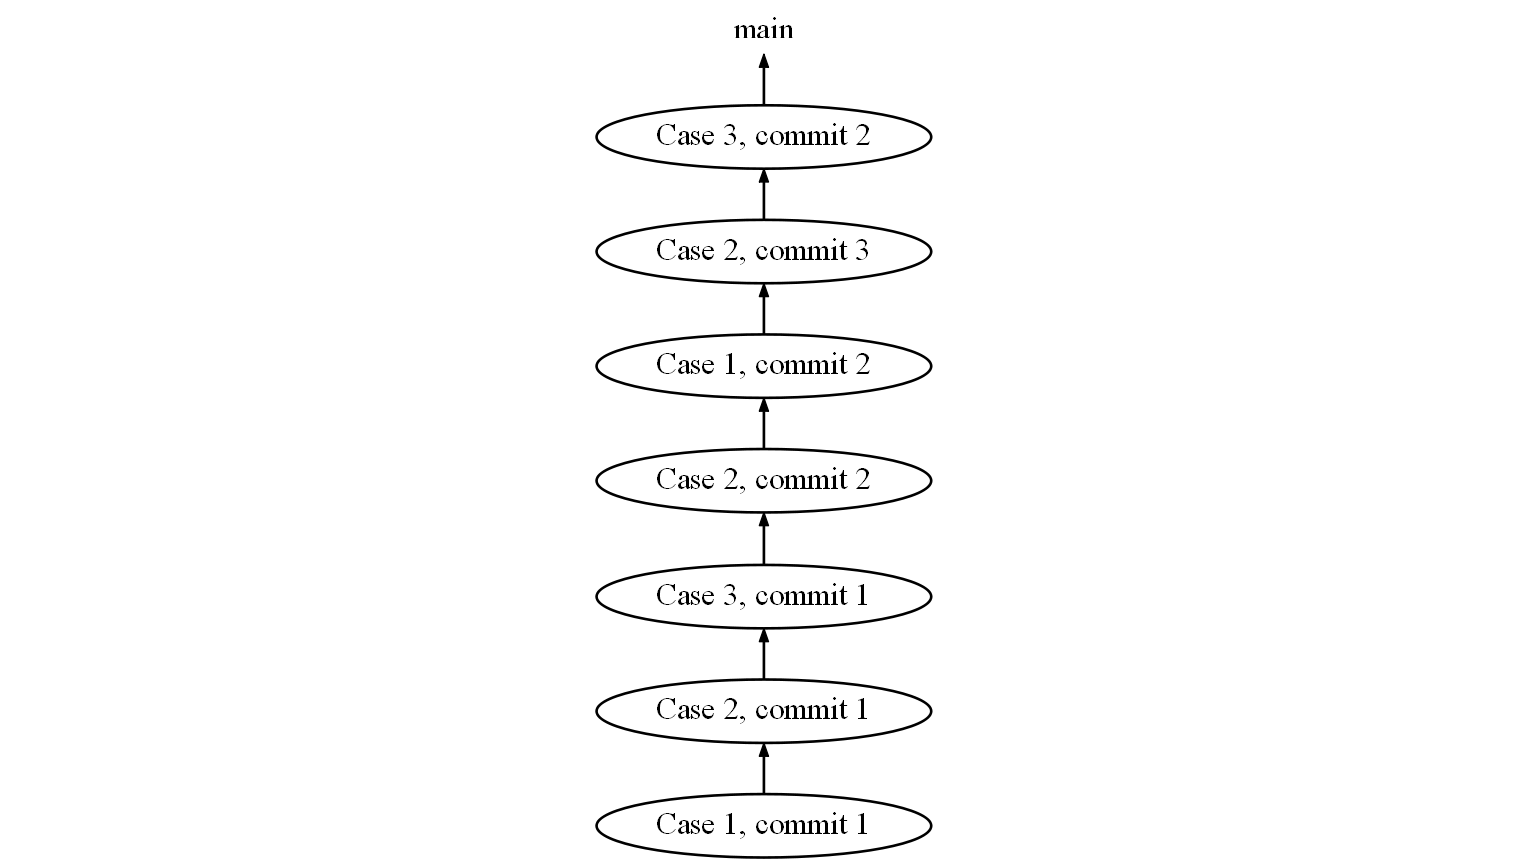
\includegraphics[scale=0.2]{02_2014_only-main.png}
\end{figure}

При ветвлении коммиты группируются по кейсам:
\begin{figure}[h!]
  \centering
  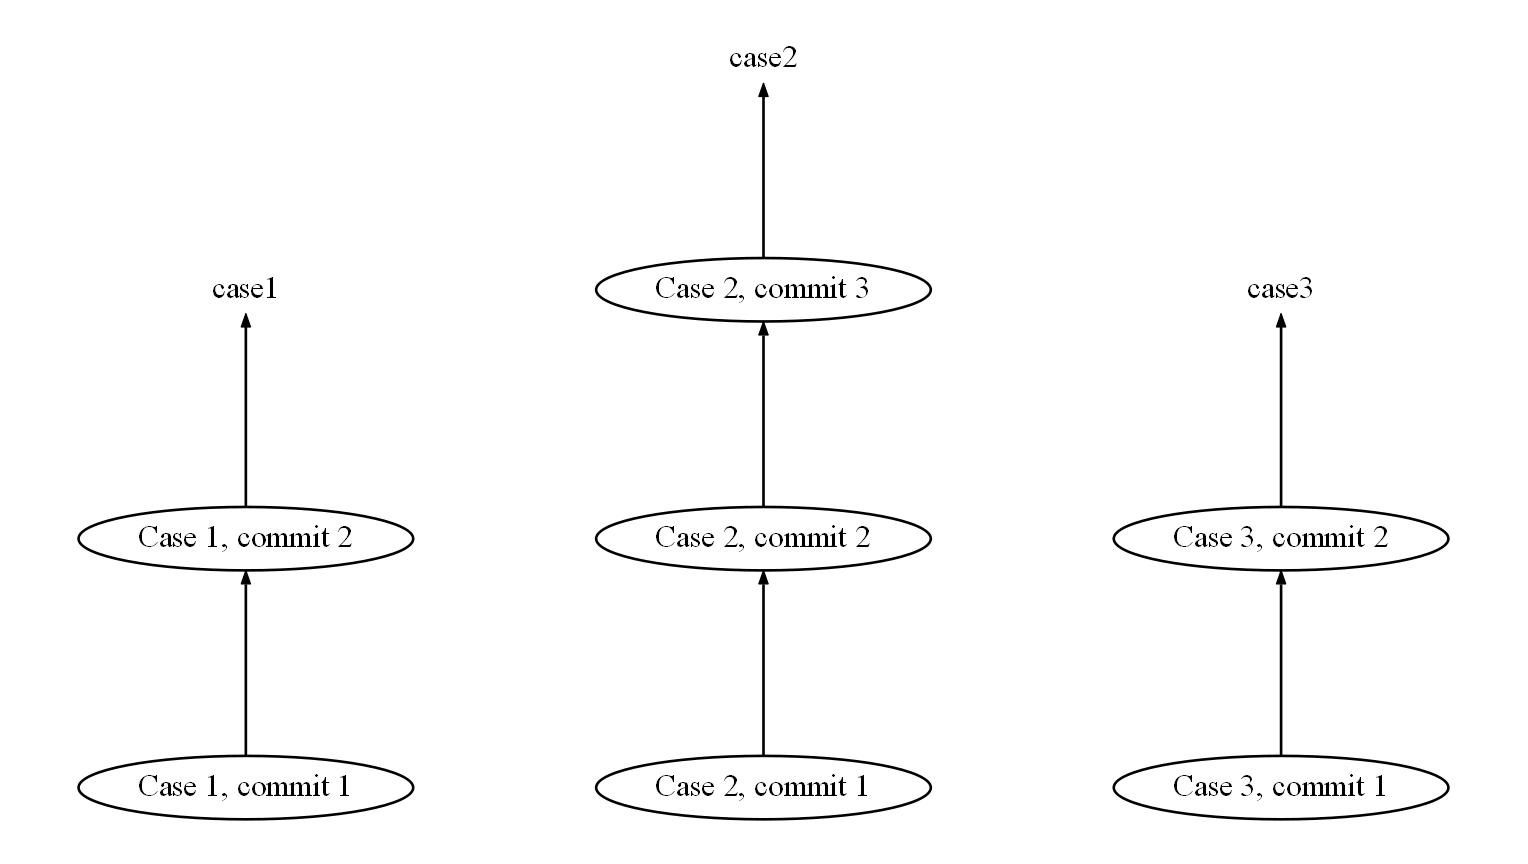
\includegraphics[scale=0.2]{02_2014_branches.png}
\end{figure}

\subsubsection*{Rebasing}

Rebasing может применяться в процессе работы над кейсом, а также для доставки коммитов в mainline.

Rebasing в процессе работы позволяет:

\begin{itemize}
  \item Получить ответвление от обновлённого mainline.
  \item Разрешать merge-conflicts небольшими порциями в ходе работы, а не одним большим куском в самом конце.
  \item Тестировать код своего кейса относительно нового mainline без его доставки в этот самый mainline.
\end{itemize}

Rebase вместо Merge как метод доставки кода в mainline позволяет получить:

\begin{itemize}
  \item Линейную историю в VCS. Линия проще и наглядней графа.
  \item Меньше проблем с blame, bisect и revert. Эти команды работают лучше на коммитах с одним родителем, чем с несколькими.
  \item Возможность удалять очень старые ветки (и их коммиты) из репозитория. Это повышает быстродействие репозитория. А если эти ветки всё-таки нужны "--- их можно хранить в архивном репозитории или в бэкапе. Тем, кто считает замедление репозитория при увеличении количества коммитов надуманной проблемой, есть смысл ознакомиться с исследованием Facebook \cite{Hlebnikov1}.
\end{itemize}

При доставке кода в mainline через Merge, mainline состоит в основном из merge-коммитов:
\begin{figure}[h!]
  \centering
  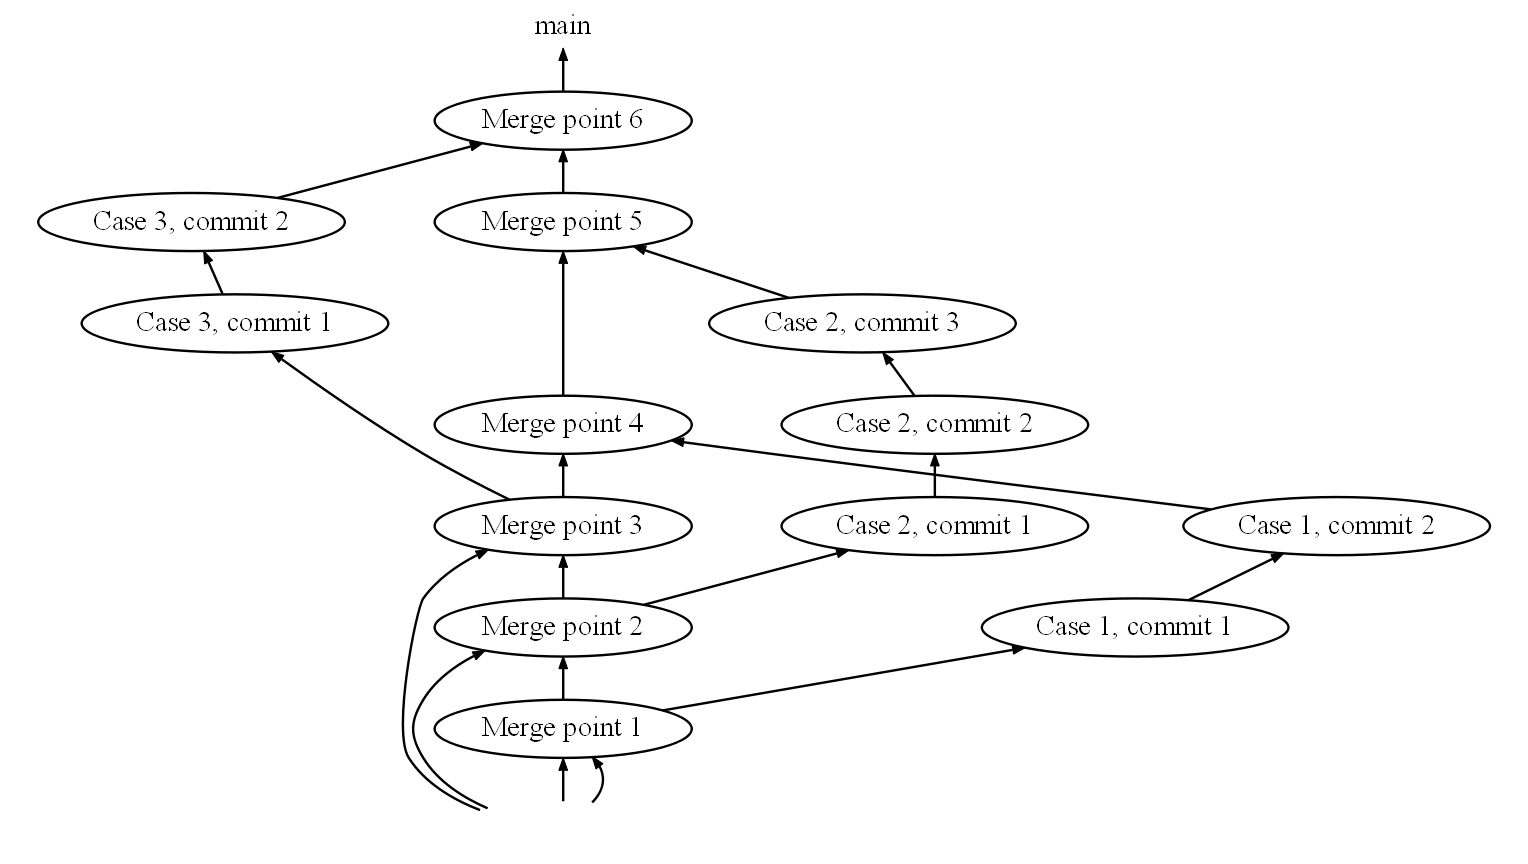
\includegraphics[scale=0.2]{02_2014_main-merged.png}
\end{figure}

Тот же самый граф, но без ярко выраженного вертикального mainline:
\begin{figure}[h!]
  \centering
  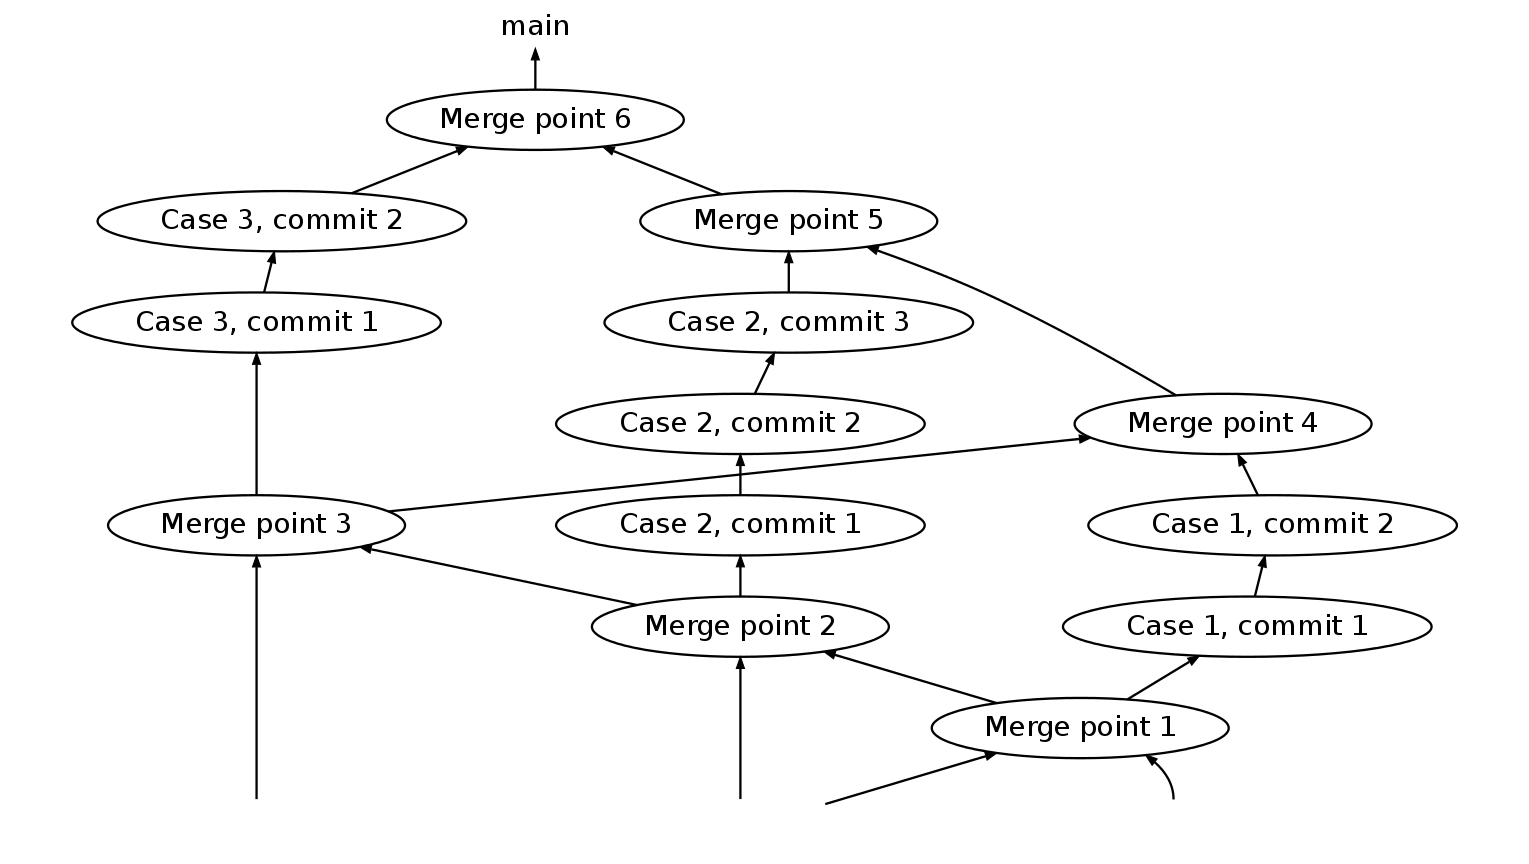
\includegraphics[scale=0.2]{02_2014_main-merged-weak-mainline.png}
\end{figure}

Как видно, в такой истории довольно трудно разобраться, особенно по прошествии долгого времени, или если разбирающийся "--- новый человек на проекте. В этом графе даже mainline трудно найти.

А вот история, которая получается при Rebase:
\begin{figure}[h!]
  \centering
  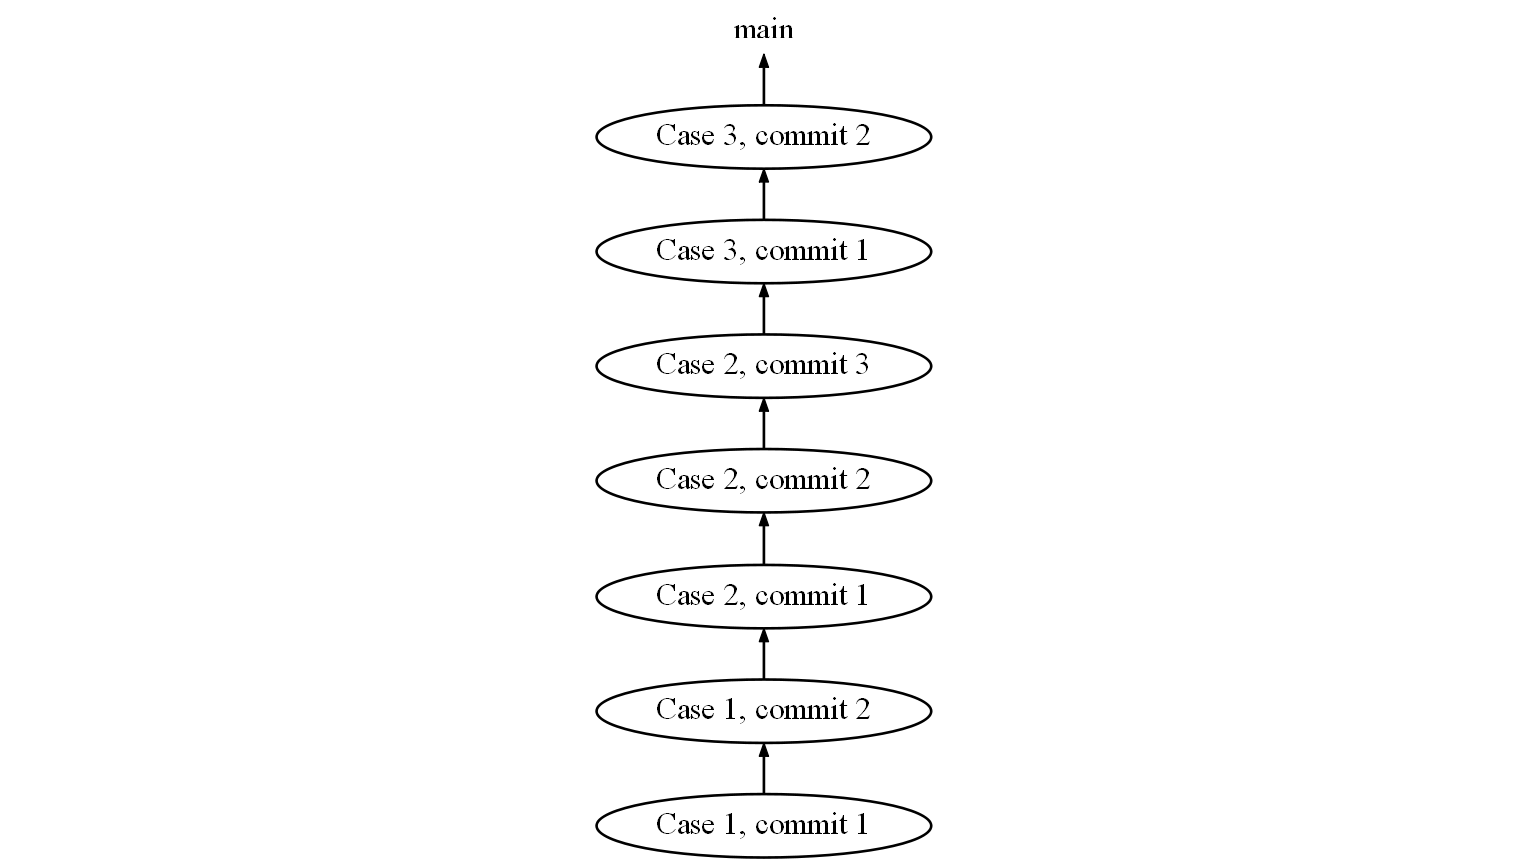
\includegraphics[scale=0.2]{02_2014_main-ordered.png}
\end{figure}

Как видно, история линейна, что сильно улучшает её читаемость. Но можно сделать ещё лучше "--- уменьшить количество коммитов. И в этом поможет squashing.

\subsubsection*{Squashing}

Squashing "--- это слияние нескольких коммитов в один. Squashing позволяет получить:

\begin{itemize}
  \item Компактную историю. Это тем важнее, чем дольше идёт разработка и чем больше коммитов собралось в репозитории.
  \item Меньше мусора в истории.
  \item Более лёгкий откат изменений.
\end{itemize}

Если после работы над кейсом ветка содержит много мусора в истории\ldots{}
\begin{figure}[h!]
  \centering
  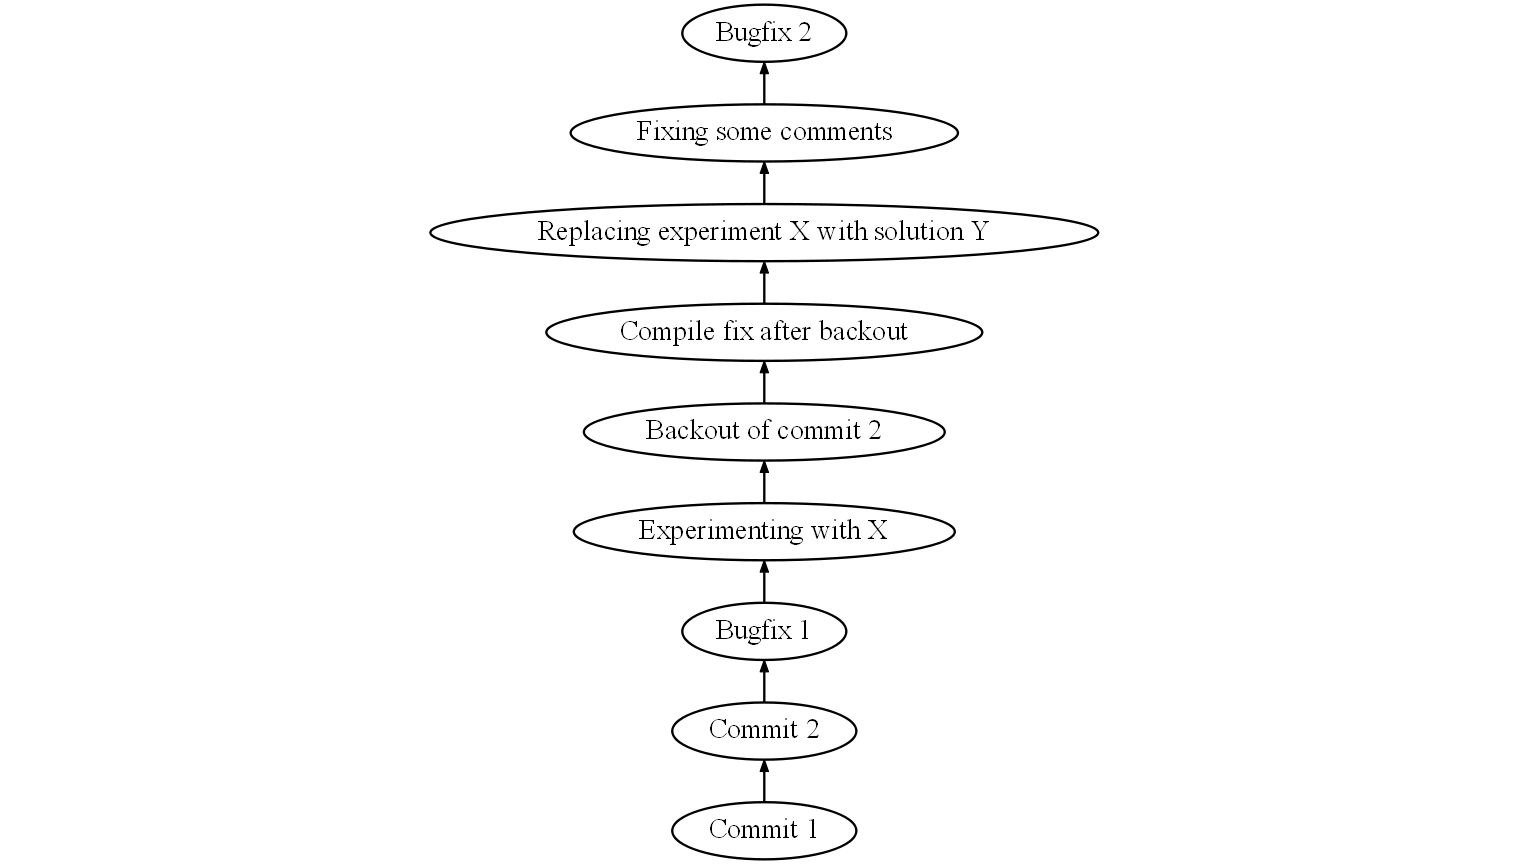
\includegraphics[scale=0.2]{02_2014_history-with-garbage.png}
\end{figure}

\ldots{}squashing позволит избавиться от этого мусора, слив все комиты в один:
\begin{figure}[h!]
  \centering
  
\includegraphics[scale=0.3]{02_2014_history-without-garbage.png}
\end{figure}

\subsection*{Конкретные команды, шаг за шагом}

Приведем примеры команд для Git и Mercurial в виде таблицы:

\begin{table}
  \centering
  \begin{tabular}{P{2.5cm}|P{3.5cm}|P{3.5cm}}
    \hline
                                  ~  & \textbf{Git}                   & \textbf{Mercurial}          \\ \hline
    Ответвление от mainline          & git checkout -{}-b case4       & hg book case4              \\
    Работа над кейсом                & git commit -m "Commit 1" \newline
                                       git commit -m "Commit 2" \ldots{}
                                                                    & hg commit -m "Commit 1" \newline
                                                                      hg commit -m "Commit 2" \ldots{} \\
    Rebase и squash              & git checkout -{}-b \emph{case4-2} \newline
                                   git rebase -{}-interactive main
                                                     & (нужны расширения rebase и histedit) \newline
                                                       hg rebase -{}-keep -{}-dest main \newline
                                                       hg histedit main \newline
                                                       hg book \emph{case4-2}      \\
    \hline
  \end{tabular}
\end{table}
Отдельно коснёмся «табу на rebase после push». Существует довольно распространённый миф, что если ветка запушена (push) на сервер "--- все возможности ребэйса (rebase) для неё потеряны, потому что если ветку проребэйсить и запушить на сервер опять (что возможно только с ключом --force), то это создаст несоответствие между репозиторием на сервере и репозиториями других разработчиков. В результате эти разработчики при попытке подтянуть эту ветку с сервера получат сломанную ветку.

На самом деле rebase возможен, если выполнять его правильно. На примере команд, приведённых в таблице, видно, что при ребэйсинге создаётся новая ветка, \textbf{case4-2}. Это принципиальный момент. Первоначальная ветка, \textbf{case4}, так и остаётся на своём месте, и получается аналог copy-on-write. Таким образом консистентность репозитория не нарушается, и ветка case4 не ломается "--- она просто устаревает. Теперь про неё можно забыть, а дальнейшую разработку, если она ещё продолжается, вести на ветке case4-2.

Также следует обратить внимание на ключ --interactive для Git и команду histedit для Mercurial. В результате их использования Git или Mercurial вызывают текстовый редактор, в котором разработчик может редактировать историю своей ветки: помечать коммиты для правки комментария, сливать несколько коммитов вместе, менять коммиты местами, удалять ненужные коммиты.

В сущности, многие коммиты "--- просто мусор в истории VCS: неудавшиеся эксперименты, багфиксы, фиксы компиляции, чистка неиспользуемых переменных, исправления опечаток в комментариях. Подобный материал в истории VCS не представляет ровным счётом никакого интереса. Как правило, от разработчика требуется имплементация фичи X или исправление бага Y, и желательно одним куском (то есть, как правило (хоть и не всегда), одним коммитом). А детали того, через что разработчик прошёл в процессе разработки, никого не интересуют. По этой причине мелкие правящие коммиты всегда имеет смысл объединить с «главными» коммитами, которые они дополняют. Это же относится и к фиксам в результате code review.

Делать слишком много «главных» коммитов для одного кейса тоже не имеет смысла. Наоборот, для большинства кейсов перед доставкой кода в mainline лучше слить все коммиты в один и использовать название кейса как комментарий этого единственного коммита. Если имел место рефакторинг без изменения функциональности "--- его имеет смысл выделить в отдельный коммит. Если имели место фиксы багов mainline'a, которые проявились при работе над данным кейсом "--- их тоже имеет смысл выделить в отдельные коммиты, и поместить эти коммиты перед основной разработкой. Других коммитов не нужно. Это и есть squashing "--- слияние нескольких коммитов в один.

Кроме чистки мусора в истории squashing также помогает убрать коммиты, которые не компилируются, путём слияния с фиксом компиляции. Это важно, если  используется bisect, а также в случае отката изменений.

Если вам захочется оставить в истории VCS свои чаяния и веяния по поводу данного кейса из ностальгических соображений "--- есть возможность сохранить их только для себя на той старой ветке case4, которая была любезно сохранена при copy-on-write-rebase. Не перетаскивая свой мусор в mainline, разработчик заодно не создает аналогичного искушения для товарищей по команде.

\subsection*{Доставка кода в mainline}

Итак, работа над кейсом завершена, код кейса оттестирован с новейшим mainline. После финальных rebase и squash на ветке должна находиться краткая и красивая история кейса, а сама ветка основана на верхушке mainline. Это и есть подходящий момент для доставки кода кейса в mainline. Для этого надо всего лишь переместить указатель mainline вперёд по ветке case4-2 "--- сделать fast-forward. Это можно сделать несколькими способами; автор предпочитает такие:

\begin{table}
  \centering
  \begin{tabular}{P{3.5cm}|P{6cm}} \hline
    \textbf{Git}                       & \textbf{Mercurial}            \\ \hline
     git push . case4-2:main      & (hg update case4-2) \linebreak
                               hg book main \linebreak  \# «book» does fast-forward \linebreak
                               \# in this case                                               \\ \hline
  \end{tabular}
\end{table}
Важно обратить внимание на точку после git push. Она означает «текущий репозиторий». Однако можно пушить и сразу в origin:

git push origin case4-2:main

При этом не следует опасаться поломки origin/main, т.к. если предлагаемый push не fast-forward, Git не позволит выполнить push без ключа -{}-force.

\subsection*{Выводы}

В результате использования предложенного подхода мы получаем:

\begin{itemize}
  \item Удобство разработки на отдельных ветвях.
  \item Возможность всегда работать и тестировать свои изменения относительно новейшего mainline.
  \item Линейную историю.
  \item Группировку коммитов по кейсам.
  \item Безупречную и компактную историю без мусора.
\end{itemize}

\begin{figure}[h!]
  \centering
  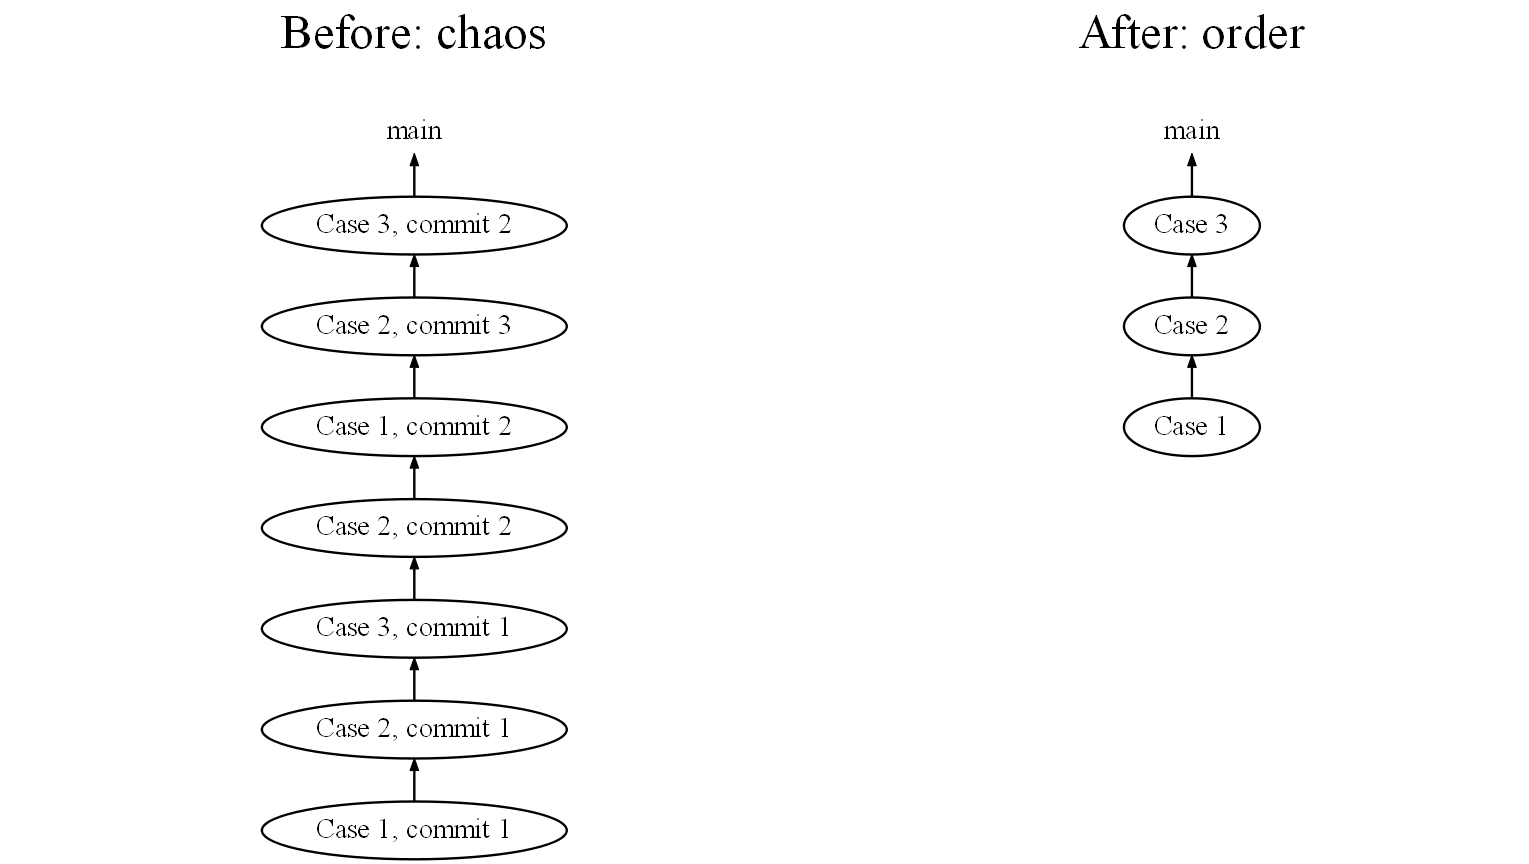
\includegraphics[scale=0.2]{02_2014_before-vs-after.png}
\end{figure}

\begin{thebibliography}{9}
\bibitem{Hlebnikov1} \url{http://thread.gmane.org/gmane.comp.version-control.git/189776}
\end{thebibliography}
\end{document}

\documentclass[10pt, a5paper]{article}
\usepackage{pdfpages}
\usepackage{parallel}
\usepackage[T2A]{fontenc}
\usepackage{ucs}
\usepackage[utf8x]{inputenc}
\usepackage[polish,english,russian]{babel}
\usepackage{hyperref}
\usepackage{rotating}
\usepackage[inner=2cm,top=1.8cm,outer=2cm,bottom=2.3cm,nohead]{geometry}
\usepackage{listings}
\usepackage{graphicx}
\usepackage{wrapfig}
\usepackage{longtable}
\usepackage{indentfirst}
\usepackage{array}
\newcolumntype{P}[1]{>{\raggedright\arraybackslash}p{#1}}
\frenchspacing
\usepackage{fixltx2e} %text sub- and superscripts
\usepackage{icomma} % коскі ў матэматычным рэжыме
\PreloadUnicodePage{4}

\newcommand{\longpage}{\enlargethispage{\baselineskip}}
\newcommand{\shortpage}{\enlargethispage{-\baselineskip}}

\def\switchlang#1{\expandafter\csname switchlang#1\endcsname}
\def\switchlangbe{
\let\saverefname=\refname%
\def\refname{Літаратура}%
\def\figurename{Іл.}%
}
\def\switchlangen{
\let\saverefname=\refname%
\def\refname{References}%
\def\figurename{Fig.}%
}
\def\switchlangru{
\let\saverefname=\refname%
\let\savefigurename=\figurename%
\def\refname{Литература}%
\def\figurename{Рис.}%
}

\hyphenation{admi-ni-stra-tive}
\hyphenation{ex-pe-ri-ence}
\hyphenation{fle-xi-bi-li-ty}
\hyphenation{Py-thon}
\hyphenation{ma-the-ma-ti-cal}
\hyphenation{re-ported}
\hyphenation{imp-le-menta-tions}
\hyphenation{pro-vides}
\hyphenation{en-gi-neering}
\hyphenation{com-pa-ti-bi-li-ty}
\hyphenation{im-pos-sible}
\hyphenation{desk-top}
\hyphenation{elec-tro-nic}
\hyphenation{com-pa-ny}
\hyphenation{de-ve-lop-ment}
\hyphenation{de-ve-loping}
\hyphenation{de-ve-lop}
\hyphenation{da-ta-ba-se}
\hyphenation{plat-forms}
\hyphenation{or-ga-ni-za-tion}
\hyphenation{pro-gramming}
\hyphenation{in-stru-ments}
\hyphenation{Li-nux}
\hyphenation{sour-ce}
\hyphenation{en-vi-ron-ment}
\hyphenation{Te-le-pathy}
\hyphenation{Li-nux-ov-ka}
\hyphenation{Open-BSD}
\hyphenation{Free-BSD}
\hyphenation{men-ti-on-ed}
\hyphenation{app-li-ca-tion}

\def\progref!#1!{\texttt{#1}}
\renewcommand{\arraystretch}{2} %Іначай формулы ў матрыцы зліпаюцца з лініямі
\usepackage{array}

\def\interview #1 (#2), #3, #4, #5\par{

\section[#1, #3, #4]{#1 -- #3, #4}
\def\qname{LVEE}
\def\aname{#1}
\def\q ##1\par{{\noindent \bf \qname: ##1 }\par}
\def\a{{\noindent \bf \aname: } \def\qname{L}\def\aname{#2}}
}

\def\interview* #1 (#2), #3, #4, #5\par{

\section*{#1\\{\small\rm #3, #4. #5}}

\def\qname{LVEE}
\def\aname{#1}
\def\q ##1\par{{\noindent \bf \qname: ##1 }\par}
\def\a{{\noindent \bf \aname: } \def\qname{L}\def\aname{#2}}
}

\begin{document}
\title{Надёжные ссылки}
\author{Юрий Андреев, Санкт-Петербург, РФ\footnote{\url{andreev.yurij@gmail.com}, \url{http://lvee.org/ru/abstracts/150}}}
\maketitle
\begin{abstract}
The rights to study and modify free software imply access to its source code.
The rights to verify scientific result imply access to its background and
previous results. That could be a problem if an access was given by a (url-)link.
The problem will be considered in the present article.
\end{abstract}

\subsection*{Обзор}
 
Свободное Программное Обеспечение (СПО) предполагает доступность исходного 
кода. Это отражает научный подход разработки ПО, при 
котором любой результат должен быть верифицируемым и открытым для 
критики. В этом смысле программный код является аналогом
научной публикации. Что же касается самих 
научных публикаций и публикации на тему СПО, то они предполагают 
доступность своих источников \emph{a priori}.   
Однако, с появлением сети Интернет, источники всё чаще указываются
в виде URL"=ссылок, которые могут стать недоступными чисто технически.
И было бы обидно <<засекретить>> результат работы таким образом. 

Каждый день в глобальной сети появляются миллионы новых  ссылок.
И  каждый  день  миллионы  ссылок  становятся  битыми "--- то   есть
указывающими на недоступный или на неверный ресурс. Эти изменения  "---
простое следствие динамичности  сети.  И  наличие  таких   временных
окон доступности ресурсов нужно  учитывать  при  проектировании  ПО,
подборке используемых  библиотек,  внедрении  удаленных  сервисов  и
контента; также тема битых ссылок постоянно обсуждается  в  связи  с
вопросами  поисковой  оптимизации  (SEO).   Учитываться  это   может
совершенно по разному.  К  примеру,  появился  «социальный»  сервис,
\texttt{snapchat.com}, принципиально  не  сохраняющий  контент  и  
ссылок  на него  "--- и  сразу  нашел  себе  пользователя.  
Нас  будет  интересовать
противоположная  ситуация,  и  ситуация  эта  будет  рассмотрена   в
контексте научных и научно-технических публикаций. Действительно,  в
этом случае желательно, чтобы ссылки указывали  на  верный  материал
когда бы статья ни была прочитана. Потеря же  ссылки  на  предыдущий
результат  в  научной  публикации  ставит  под   сомнение   верность
текущего  результата (тут  можно  вспомнить  про  Великую  Теорему
Ферма,  которая  более  трёхсот  лет  оставалась  гипотезой,   из-за
«недоступности» оригинального доказательства /если оно было/).

А  ссылки  появляются  везде.  Автор  лично  присутствовал   на
серьезной математической конференции,  где  один  из  докладчиков  в
своем выступлении приводил переписку из  ночного  чата.

Доступность материалов  в  библиотеке,  вообще  говоря,  кажется
более стабильной,  чем  в  интернете.  В  библиотеке найдется всё,
если... к примеру, не сгорит (однажды в Библиотеке Академии  Наук 
\cite{AY2}
автору довелось читать статью из сборника, который, судя  по  надписям  и  штампам,
сначала тонул в наводнении 1824 года, а потом горел  в  пожаре  1988
года). Более того,  существуют  системы  обязательного  хранения. 
С момента своего основания, Национальная Библиотека Беларуси
стала получать два обязательных бесплатных экземпляра белорусских 
изданий и один обязательный бесплатный экземпляр изданий, 
выходивших в СССР (РФ) до марта 1995 г, библиотека также является 
депозитарием материалов ООН и других 
международных организаций \cite{AY3}. То же можно сказать про 
Российскую    Государственную    Библиотеку \cite{AY4}. 
Важно  понять,  что
найдя нужную книгу, мы сразу можем начать читать, то  есть  получаем
доступ к её содержанию.

    С появлением компьютеров возник вопрос физической доступности  —
нельзя  считывать  информацию  напрямую.   А   носители   информации
меняются очень быстро,  и  с  магнитной  пленки,  да  и  с  дискеты,
информацию  теперь  прочитать  будет   крайне   затруднительно
\footnote{Однако, развитие идёт по спирали "--- утрату большой части
античного письменного наследия связывают также со сменой
технологий, так как множество текстов никогда не переписывалось с
папирусов на пергаментные кодексы \cite{AY5}.}. 
С появлением  интернета  вопрос  сохранения  копированием  стал  менее
актуален. Теперь вопрос сохранности информации  предстает  в  другом
разрезе "--- в проблеме контроля за её доступностью.

\subsection*{Терминология}

Уточним терминологию. Мы будем рассматривать URL"=\textit{ссылки}, но в  более
общем смысле "--- как  ссылки  на  внешние,  по  отношению  к  материалу,
ресурсы       (ссылки       в       тексте,       из        разделов
<<ссылки>>, <<библиография>>, <<литература>>). Ссылка указывает  на  ресурс.
\textit{Ресурс} "--- это может быть какой-либо  контент,  сервис,  или  печатная
статья, книга. 
\textit{Надёжность ссылки} "--- способность указывать на верный, доступный 
ресурс.  

\subsection*{Классификация}

Классифицируем  ссылки  по  степени
надёжности (c  допуском  на  то,  что  это  достаточно  
индивидуальный  вопрос, особенно для внутренних ссылок).
Перечислим возможные варианты по степени убывания надёжности.
\begin{itemize}
\item Ссылки на части в оригинальном материале кажутся надёжными по 
определению, если это не документ, страницы из которого могут <<выпасть>>.  
\item Разумеется, стабильнее всего ссылки,  принадлежащие  организациям,
отвечающим за их распределение и обслуживающим интернет:  
\texttt{icann.org,  w3.org,  example.com,...}
\item Сайты сообществ, таких как \texttt{gnu.org,  ctan.org}, специальные
архивы \texttt{arxiv.org}, университетские сайты, \texttt{<site>.edu}
\item Правительственные  сайты,   сайты   больших   компаний   (правда
бывает... в 1999  году  компания  Microsoft  забыла  продлить  домен
\texttt{passport.com},  что  привело  к  недоступности  Hotmail  для   многих
пользователей; видимо, этот случай  не  послужил  Microsoft  уроком,
поскольку в 2003 году компания снова забыла продлить  важный  домен,
на этот раз \texttt{hotmail.co.uk}\cite{AY1}).
\item Нужно  учитывать  различные  характеристики:  есть  ли  архив   у
новостного сайта, сколько подписчиков и форков у проекта  на  github
и т.~п.
    Вообще говоря, доступность  материала  по  ссылке "---  это  также
вопрос доступности сервиса, на  котором  этот  материал  расположен.
Одно дело, если проект расположен на github, другое дело "--- на  каком-либо
частном ресурсе,  который  может  закрыться.  Пример  "---  закрывшаяся
почта  @london.com  (кстати,  там  был  и  платный  сервис).  Автор,
указавший ее в контактах, станет недоступен.
\item При ссылке  на  Википедию  нужно  учитывать,  что  материал  может
измениться. Понятно, что это не всегда  желательно.  При  ссылке  на
github обычно важнее  само  наличие  контента,  и в  большинстве
случаев он, наоборот, должен изменяться.
\item Блоги.  Иногда  достаточно   постоянные,   зависит   от   автора.
Социальные сервисы в  этом  плане  намного динамичнее,  доступность
гораздо  хуже  (не  говоря  о  том,  что  доступность  может  просто
регулироваться закрытостью для незарегистрированных  пользователей).
На отдельном авторском блоге материалы  могут  представлять  большую
ценность для автора,  он  заинтересован  в  сохранении  доступности.
Хотя всегда есть вероятность, что имя не будет продлено.
\end{itemize}

Графически степень надёжности ссылок в пределах 
одного сайта можно изобразить в виде треугольной диаграммы (рис. 1).
Обычно, над корнем находятся основные ссылки (1), 
выше "--- контент сайта (2),
еще выше "--- пользовательский контент (3).   

\begin{figure}[h!]
  \centering
  \includegraphics[scale=0.8]{01_2015_diagram.pdf}
\end{figure}

Выделим <<центр тяжести>> и составим общую диаграмму надёжности, 
соответствующую нашей классификации (рис. 2). 
Самые надёжные ссылки располагаются внизу. Ссылки с верхних слоёв 
легко сдуваются ветром перемен.

\subsection*{Структура ссылок и алгоритм поиска}

При выборе ссылки важно учитывать её структуру. Вкратце остановимся на этом.
Рассмотрим ссылку вида:

\texttt{http://<site-name>.tld/<section>/<page-name>?<query>}

Если ссылка становится недоступной, то, куда мы попадём,  зависит  от
организации  редиректа   (перенаправления)   на   сайте.   Возможные
варианты: это  будет  страница с ошибкой,  главная  станица  или
страница  вышележащего  раздела;  лучший  вариант  "---   редирект   на
актуальный адрес. Обычный алгоритм поиска таков:

\noindent
1. Ищем информацию на доступных ссылках сайта (двигаясь вниз по рис.1)
\begin{itemize}
\item \texttt{http://<site-name>.tld/<section>/<page-name>}
\item \texttt{http://<site-name>.tld/<section>/}
\item \texttt{http://<site-name>.tld}
\end{itemize}
2. Через «поиск»
\begin{itemize}
\item поиск \texttt{<section>, <page-name>} по сайту, если возможно
\item google \texttt{<site-name>, <section>, <page-name>}
\item поиск исходя из контекста, в котором ссылка была указана.
\end{itemize}
3. Поиск <<следов>> информации в сети: сервис 
\texttt{archive.org}, кэши поисковых систем 
\footnote{Отдельная тема. Наличие в кэше зависит 
от частоты индексации, настроек robots.txt, самой поисковой системы и др.
Время снимков \texttt{archive.org} не связано с изменениями на сайте, о чём они 
сразу честно предупреждают.}.

Плохо, если  \texttt{<site-name>, <section>, <page-name>} 
не  несут  информации  (это, кстати, правило SEO).

К  примеру, \url{http://www.red-bean.com/kfogel/948.html}  
\footnote{На самом деле, это контрпример, там написано как раз об этом.}
(заметьте, данный пример остается актуальным в рамках  этой  статьи  даже  если
ссылка  станет  недоступной).  Поэтому  следует приводить такие ссылки с
поясняющей информацией.

\subsection*{Примеры ссылок из сборника}
Приведем несколько интересных ссылок из сборника \cite{AY5}:
\begin{itemize}
\item классическая ссылка: 
The GNU Project Debugger, \url{http://www.gnu.org/software/gdb/}
\item ссылка с датой просмотра: 
\url{http://www.blendernation.com/} Дата просмотра: 20.04.2014
\item сокращенная ссылка: \url{http://bit.ly/1sk1bZt}

Сервис bit.ly позволяет сокращать ссылки, делая из длинной
непонятной короткую непонятную. Хранит он ссылки вечно, но не
стоит забывать, что это всего лишь ссылка на ссылку. Она увеличивает
читабельность, но не надёжность.
\end{itemize}

\subsection*{Правила подбора ссылок}
Сформулируем правила подбора надёжных ссылок.
\begin{itemize}
\item Иногда следует добавлять информацию к ссылке, она может помочь, как 
в поиске информации, так и в понимании её актуальности.
\item Иногда следует включить материал в саму статью. К примеру, когда
материал "--- это чья-та цитата, размещенная на блоге (в 
истории про Microsoft, описанной выше, непонятно, какую ссылку
давать, но <<гуглится>> хорошо).
\item Из различных представлений одной ссылки выбираем более читабельное.
Для нечитабельных можно воспользоваться сервисами преобразования ссылок, 
при условии надёжности последних. Иногда лучше давать \textit{структурную} ссылку 
(см. пример \cite{AY3}).
\item Если есть выбор из нескольких ссылок, указывающих на один ресурс,
выбираем наиболее надёжную.
\item Если есть выбор между ссылкой на печатное издание или электронное,
выбираем обе.
\item Нужно исходить из актуальности основного материала и 
здравого смысла. Однако, значимость материала может недооцениваться 
автором, поэтому, если есть возможность, лучше давать более надёжную 
ссылку. 
\item Хорошо само существование раздела ссылок. Сам по себе, 
этот раздел помогает понимать общий контекст материала
в предметной области.  

\end{itemize}


\begin{thebibliography}{9}
\bibitem{AY1} \url{http://google.com}
\bibitem{AY2} \url{https://ru.wikipedia.org/wiki/}\\ \texttt{Библиотека\_Российской\_ академии\_наук}
\bibitem{AY3} Национальная Библиотека Беларуси, \url{http://nlb.by}, \texttt{главная $\to$ информационные ресурсы $\to$ фонды и коллекции библиотеки}
\bibitem{AY4} \url{https://ru.wikipedia.org/wiki/}\\ \texttt{Российская\_государственная\_библиотека},\\ 
см. также федеральный закон РФ <<Об обязательном экземпляре документов>> от 29.12.1994 № 77-ФЗ
\bibitem{AY5} \url{https://ru.wikipedia.org/wiki/}\\ \texttt{Книжные\_утраты\_в\_Поздней\_античности\_и\_«Тёмных\_веках»}
\bibitem{AY6} Материалы международной конференции Linux Vacation / Eastern
Europe (LVEE 2014), \url{http://lvee.org/ru/reports/materials_lvee_2014}
\end{thebibliography}

\end{document}

\documentclass[10pt, a5paper]{article}
\hyphenation{GNU-Plot}
\usepackage{pdfpages}
\usepackage{parallel}
\usepackage[T2A]{fontenc}
\usepackage{ucs}
\usepackage[utf8x]{inputenc}
\usepackage[polish,english,russian]{babel}
\usepackage{hyperref}
\usepackage{rotating}
\usepackage[inner=2cm,top=1.8cm,outer=2cm,bottom=2.3cm,nohead]{geometry}
\usepackage{listings}
\usepackage{graphicx}
\usepackage{wrapfig}
\usepackage{longtable}
\usepackage{indentfirst}
\usepackage{array}
\newcolumntype{P}[1]{>{\raggedright\arraybackslash}p{#1}}
\frenchspacing
\usepackage{fixltx2e} %text sub- and superscripts
\usepackage{icomma} % коскі ў матэматычным рэжыме
\PreloadUnicodePage{4}

\newcommand{\longpage}{\enlargethispage{\baselineskip}}
\newcommand{\shortpage}{\enlargethispage{-\baselineskip}}

\def\switchlang#1{\expandafter\csname switchlang#1\endcsname}
\def\switchlangbe{
\let\saverefname=\refname%
\def\refname{Літаратура}%
\def\figurename{Іл.}%
}
\def\switchlangen{
\let\saverefname=\refname%
\def\refname{References}%
\def\figurename{Fig.}%
}
\def\switchlangru{
\let\saverefname=\refname%
\let\savefigurename=\figurename%
\def\refname{Литература}%
\def\figurename{Рис.}%
}

\hyphenation{admi-ni-stra-tive}
\hyphenation{ex-pe-ri-ence}
\hyphenation{fle-xi-bi-li-ty}
\hyphenation{Py-thon}
\hyphenation{ma-the-ma-ti-cal}
\hyphenation{re-ported}
\hyphenation{imp-le-menta-tions}
\hyphenation{pro-vides}
\hyphenation{en-gi-neering}
\hyphenation{com-pa-ti-bi-li-ty}
\hyphenation{im-pos-sible}
\hyphenation{desk-top}
\hyphenation{elec-tro-nic}
\hyphenation{com-pa-ny}
\hyphenation{de-ve-lop-ment}
\hyphenation{de-ve-loping}
\hyphenation{de-ve-lop}
\hyphenation{da-ta-ba-se}
\hyphenation{plat-forms}
\hyphenation{or-ga-ni-za-tion}
\hyphenation{pro-gramming}
\hyphenation{in-stru-ments}
\hyphenation{Li-nux}
\hyphenation{sour-ce}
\hyphenation{en-vi-ron-ment}
\hyphenation{Te-le-pathy}
\hyphenation{Li-nux-ov-ka}
\hyphenation{Open-BSD}
\hyphenation{Free-BSD}
\hyphenation{men-ti-on-ed}
\hyphenation{app-li-ca-tion}

\def\progref!#1!{\texttt{#1}}
\renewcommand{\arraystretch}{2} %Іначай формулы ў матрыцы зліпаюцца з лініямі
\usepackage{array}

\def\interview #1 (#2), #3, #4, #5\par{

\section[#1, #3, #4]{#1 -- #3, #4}
\def\qname{LVEE}
\def\aname{#1}
\def\q ##1\par{{\noindent \bf \qname: ##1 }\par}
\def\a{{\noindent \bf \aname: } \def\qname{L}\def\aname{#2}}
}

\def\interview* #1 (#2), #3, #4, #5\par{

\section*{#1\\{\small\rm #3, #4. #5}}

\def\qname{LVEE}
\def\aname{#1}
\def\q ##1\par{{\noindent \bf \qname: ##1 }\par}
\def\a{{\noindent \bf \aname: } \def\qname{L}\def\aname{#2}}
}

\begin{document}
\title{Гибкая графика \LaTeX}
\author{Юрий Андреев, Санкт-Петербург, РФ\footnote{\url{andreev.yurij@gmail.com}, \url{http://lvee.org/ru/abstracts/151}}}
\maketitle
\begin{abstract}
Classification of the different types of graphics elements will be given. 
Mixed methods to work with graphics within \LaTeX \, system are examined.
A brief overview of the appropriate tools and tips are given as well.
\end{abstract}        

\section*{Введение}

Система вёрстки \LaTeX \cite{RG1} теоретически обладает неограниченными возможностями по 
набору сложных документов. Подключение соответствующих пакетов позволяет отображать такие 
сложные объекты как ноты и структурные химические формулы.   
Наиболее востребованной является возможность быстрого набора 
сложных математических формул 
(типа $\displaystyle{\oint_{\gamma} f(z)dz = 2\pi i \sum_k Res(f, a_k)}$ 
\footnote{формула вычетов, называется среди самых красивых математических формул. 
Первое место в подобных опросах обычно занимает тождество Эйлера $e^{i\pi}=-1$.}
и сложнее).
О графике \LaTeX \, можно написать книгу\cite{RG2}, в данной же статье хотелось бы заострить внимание на следующей проблеме.

Графика --- область чрезвычайно обширная. 
Многие графические элементы, типа перечисленных выше, создаются по чётко определённым правилам и поэтому 
могут быть эффективно описаны на каком-либо языке.
С другой стороны, есть элементы, требующие повышенной гибкости редактирования,
правила создания которых заранее не известны.
И в таких случаях применение программного подхода становится практически
\footnote{надо понимать не как оборот речи, а в прямом смысле. Теоретическая возможность остаётся.}
невозможным. 
Далее мы дадим классификацию элементов по типу редактирования 
и кратко опишем несколько практических приёмов работы с графикой
\footnote{описанные далее WYSIWYG (What You See Is What You Get) редакторы являются кроссплатформенными}
в рамках системы \LaTeX.

\section*{Графика по правилам и без}
\subsection*{1. Генерируемая графика}

Когда графический элемент может быть сгенерирован, он обычно описывается на языке одного из 
прикладных пакетов: R, GNUPlot, Graphviz, ROOT, Maple, Sage и др. 
Если нам нужно будет использовать полученные результаты в latex-документе, то 
их всегда можно экспортировать в форматы \texttt{ps, pdf} и
затем вставить в latex-документ с помощью пакета \texttt{graphics}.
Этот способ можно назвать \textit{обобщением}, так как экспорт производится в формат более широкого назначения. 
Но при его использовании теряется информация (читаемость). 
Поэтому, для возможности последующего редактирования и более удобного взаимодействия, 
для сохранения исходного кода, для поддержки единой стилистики,
пакеты обычно предоставляют способы интеграции с \LaTeX \,
-- \textit{конвертацию} (преобразование кода одного языка в другой) и \textit{внедрение} 
(использование кода одного языка в другом).

Это может быть экспорт в latex-формат или преобразование в формат одного из latex-пакетов.
Например, для вывода из GNUPlot в latex-формат нужно указать соответствующий обработчик\footnote{ориг. термин: \textit{terminal}}  
\texttt{set term latex} и файл вывода \texttt{set output ``plot.tex''}. 
Доступны различные варианты, \texttt{set term pstricks}, \texttt{set term epslatex} и др.

При использовании \texttt{epslatex} возможно внедрение latex надписей внутри gnuplot-файла командой 
\texttt{set label}. Это позволяет получить на выходе (\texttt{output}) два файла 
plot.eps и включающий его plot.tex, который уже при latex компиляции выдаёт графику с точно 
позиционированными поверх неё latex-надписями.\footnote{WYSIWYG-добавление latex-надписей обсуждается 
в третьей части этой секции.}     

Напротив, существует практика внедрения результатов работы прикладного пакета в latex-документ
с помощью подключения специального latex-пакета. Для GNUPlot есть latex-пакет \texttt{gnuplottex},
для Sage -- \texttt{sagetex}. Также, нельзя не упомянуть про \texttt{psfrag} и другие latex-пакеты для
работы с EPS-форматом.    

В заключении сделаем два замечания. 
Во-первых, при любом внедрении усложняется процесс компиляции. 
В случае с \texttt{gnuplottex} нужно использовать ключ компиляции: \texttt{pdflatex -shell-escape}, 
в случае \texttt{sagetex} компиляция осуществляется в два прохода. 
Во-вторых, ограничиваются возможности внедряемого языка. 

\subsection*{2. Когда нужна корректировка. Ограничения против гибкости}

Иногда возможно генерировать основу графического элемента, 
но при этом будет необходимо последующее добавление или корректировка деталей. 
Также, при создании некоторых элементов, становится трудно искать и редактировать их детали --
недостатки текстового набора тут начинают перевешивать преимущества.

В качестве примера можно привести работу с таблицами, которую лучше выполнять в WYSIWYG-редакторе. 
Потом таблицу можно будет преобразовать в latex-формат напрямую, с помощью соответствующего конвертера, 
или через формат с разделителями значений (его можно обработать latex-пакетом \texttt{pgfplotstable}).     

Ещё одним примером является пакет \texttt{grafviz} (язык \texttt{dot}).
Он работает по \textit{принципу ограничивающих условий}, когда
элементы описываются рядом ограничений по характеристикам, а реальные значения этих 
характеристик вычисляются в момент генерации. Поэтому полученный результат 
может нуждаться в корректировке \cite{RG3}. Пакет используется для отображения различных зависимостей 
(в программном обеспечении от Puppet до Trac). 

Надо заметить, что для пакета возможны те же пути внедрения, что и описанные в предыдущем разделе.
Если мы для dot-файла применим конвертер dot2tex с опцией math: 
\texttt{dot2tex -tmath --autosize example.dot > example.tex}, то latex-выражения, написанные в 
dot-файле будут корректно обработаны. Будет получен tex-файл (с хорошо поясняющими комментариями)
в pstricks- и tikz-формате. (Наряду с latex-выражениями, в dot-файле можно передавать pstricks- и tikz-инструкции
внутри поддерживаемого dot атрибута style.)
Если же мы подсоединим один из latex-пакетов \texttt{dot2texi}, \texttt{graphviz}, то сможем изъясняться на языке dot внутри latex-документа
(не забываем про ключ \texttt{pdflatex -shell-escape} при компиляции).

С непосредственным WYSIWYG-редактированием dot-файлов есть проблемы, так как происходит значительная перекомпоновка 
при внесении практически любого изменения. Для получение более подробной информации о компоновке, можно 
получить расширенный dot-вывод, применив конвертер dot2tex.
Также, можно переконвертировать dot-файл в файл svg или в файл графических пакетов pstricks, tikz  
и редактировать его уже средствами из следующего раздела.


\subsection*{3. WYSIWYG подход}
% Бурбаки не прав, что надо без рисунков. Иногда можно доказать, не приводя ни одной формулы. Вообще, есть визуалы, у которых
% более развито визуальное мышление, к примеру. Схематично что-либо показать это здорово, это способ интерпретации и презентации. 
% Можно объяснить в рисунках даже ребенку. 

Если примером задачи из первого раздела могла бы быть задача построения параболы, когда  
нужно отдать на выполнение только её формулу и, возможно, границы области вывода, примером для второго раздела могла бы быть кривая Безье, 
вычисление которой происходит на основе опорных точек, координаты которых и нужно сообщить (и делать это лучше в графическом редакторе), 
то, задача этого раздела -- построение произвольного графика. Это полностью WYSIWYG-задача.
 
Перечислим несколько редакторов, от общих к специализированным, слева на право:  
Inkscape, GeoGebra, TexMacs, LatexDraw, jPicEdt\cite{RG4}.
Экспортировать редактируемое изображение в формат latex-пакета \texttt{pstricks} умеет такой известный редактор векторной графики, как Inkscape.
Другие, помимо \texttt{pstricks}, умеют экспортировать в форматы latex-пакетов, таких как \texttt{tikz}, \texttt{eepic} или в обычный \texttt{latex}.
(Не очевидно, но чтобы сохранить файл в нужном формате в jPicEdt нужно прежде определить для документа тип: Edit $\to$ Content Type. 
Тут необходимо сказать ещё про установку jPicEdt. 
Возможно, нужно будет заменить \texttt{javaw} на \texttt{java} в файле запуска: \texttt{sudo nano /usr/bin/jpicedt}.)  
Поэтому созданный в программе векторный рисунок можно без труда преобразовать в нужный формат и использовать в latex-документе.
 
Сложности начинаются, когда необходимо редактировать код одного из latex-пакетов. 
Внутреннем форматом редакторов являются форматы на основе XML, и на данный момент нет полноценной реализации импорта latex-кода. 
Казалось бы, что импорт реализован в редакторе jPicEdt, но редактор сохраняет в комментариях свой формат внутри сгенерированного latex-файла и,
видимо, использует его при импорте. (Поддержка импорта произвольного кода заявлена на сайте программы\cite{RG4}, выдаёт ошибки парсинга) 
Это полезный приём, которым можно пользоваться, для того, чтобы объединять
весь необходимый для редактирования код в одном latex-документе. Для пользователей Emacs плагин Auctex
предоставляет удобные функции: комментирование и обратное ему действие над выделенными строками 
реализовано в виде комбинации \texttt{C-c ;} подобные действия над параграфом осуществляет комбинация \texttt{C-c \%}           
Что касается LatexDraw, то в нем есть функция вставки pstricks-кода. Но пока LatexDraw распознаёт подмножество из
тех pstricks-команд, которые умеет генерировать сам.  
   
Разумеется, возможности у редакторов различны, как в области обычной графики, так и в поддержке latex-кода. 
Редактор GeoGebra отображает формулы сразу в стиле \texttt{displaystyle} (которым отображаются формулы на отдельной строке), в 
LatexDraw эту директиву нужно включать в текст. Возможность поворачивать latex-изображение в GeoGebra осуществляется 
в командной строке редактора, командой \texttt{RotateText},
в то время как в LatexDraw его можно поворачивать как обычный векторный элемент.

Также дело усложняется, если нам нужно вставить в редактируемый документ изображение из другого файла.
Это не всегда возможно, а если возможно, то при дальнейшем экспорте изображение будет включено в код как отдельный файл,
или не включено вообще. Если нас устраивает eps-файл, то тут стоит опять напомнить про пакеты 
типа \texttt{psfrag}. Выполнить графику одним pstricks-кодом всё же можно, но стандартной задачей это не является:      
% работа с растром 

\begin{figure}[h!]
  \centering
  \includegraphics[scale=0.6, angle=90]{01_2015_Andreev_graphics_fig1}
\end{figure}

% \begin{verbatim}
% \int\sqrt\exp\exp 
% \end{verbatim} 
 

\section*{Выводы}

В рамках системы \LaTeX \, возможно совместное использование текстового формата и WYSIWYG-управления, 
что позволяет добиться необходимой гибкости в редактировании графических элементов разной природы.
Такая гибкость усложняет межпрограммное взаимодействие. Накладными расходами является также необходимость
поиска подходящих конвертеров и редакторов (можно воспользоваться \cite{RG5}) и общих соглашений по работе
над конкретной задачей.  

\begin{thebibliography}{1}
\bibitem{RG1} Comprehensive \TeX \, archive network, \url{http://ctan.org}
\bibitem{RG2} <<The \LaTeX \, Graphics Companion>>, Michel Goossens, Sebastian Rahtz, Frank Mittelbach. Русскоязычная версия была выпущена 
издательством <<Мир>> в 2002 году под названием <<Путеводитель по пакету \LaTeX \, и его графическим расширениям>>. 
\bibitem{RG3} \url{https://en.wikipedia.org/wiki/DOT_(graph_description_language)}, раздел \texttt{limitations}
\bibitem{RG4} LatexDraw -- \url{http://latexdraw.sourceforge.net/}, jPicEdt \url{http://jpicedt.sourceforge.net/}  
\bibitem{RG5} \url{http://stackoverflow.com}
\end{thebibliography}



\end{document}

% Другая ветвь - Latex и OpenOffice и т.п.
% Другая ветвь - troff, texinfo, man 
% Другая ветвь - XML и другие языки разметки
% Другая ветвь - рассмотрение: автоматические действия, no-WYSIWYG и WYSIWYG; intouch/intype действия. 
% --- автоматические: компоновка текста на странице, расстановка переносов, выравнивание, 
% --- (мы сами "руками" строки не выравниваем даже в WYSIWYG редакторе)
% --- также и в WYSIWYG Zotero - (аналог bibtex), нумерация страниц.
% --- элементы WYSIWYG: AucTeX; emacs выделяет заголовки, позиционирует подчёркивания (подчеркивания появляются сразу после окончания ввода, как выравнивание строки в word сразу после перехода на следующую). Конечно, вывод на принтер будет другим, близко к more or less: WYSIMOLWYG.

\documentclass[10pt, a5paper]{article}
\usepackage{pdfpages}
\usepackage{parallel}
\usepackage[T2A]{fontenc}
\usepackage{ucs}
\usepackage[utf8x]{inputenc}
\usepackage[polish,english,russian]{babel}
\usepackage{hyperref}
\usepackage{rotating}
\usepackage[inner=2cm,top=1.8cm,outer=2cm,bottom=2.3cm,nohead]{geometry}
\usepackage{listings}
\usepackage{graphicx}
\usepackage{wrapfig}
\usepackage{longtable}
\usepackage{indentfirst}
\usepackage{array}
\newcolumntype{P}[1]{>{\raggedright\arraybackslash}p{#1}}
\frenchspacing
\usepackage{fixltx2e} %text sub- and superscripts
\usepackage{icomma} % коскі ў матэматычным рэжыме
\PreloadUnicodePage{4}

\newcommand{\longpage}{\enlargethispage{\baselineskip}}
\newcommand{\shortpage}{\enlargethispage{-\baselineskip}}

\def\switchlang#1{\expandafter\csname switchlang#1\endcsname}
\def\switchlangbe{
\let\saverefname=\refname%
\def\refname{Літаратура}%
\def\figurename{Іл.}%
}
\def\switchlangen{
\let\saverefname=\refname%
\def\refname{References}%
\def\figurename{Fig.}%
}
\def\switchlangru{
\let\saverefname=\refname%
\let\savefigurename=\figurename%
\def\refname{Литература}%
\def\figurename{Рис.}%
}

\hyphenation{admi-ni-stra-tive}
\hyphenation{ex-pe-ri-ence}
\hyphenation{fle-xi-bi-li-ty}
\hyphenation{Py-thon}
\hyphenation{ma-the-ma-ti-cal}
\hyphenation{re-ported}
\hyphenation{imp-le-menta-tions}
\hyphenation{pro-vides}
\hyphenation{en-gi-neering}
\hyphenation{com-pa-ti-bi-li-ty}
\hyphenation{im-pos-sible}
\hyphenation{desk-top}
\hyphenation{elec-tro-nic}
\hyphenation{com-pa-ny}
\hyphenation{de-ve-lop-ment}
\hyphenation{de-ve-loping}
\hyphenation{de-ve-lop}
\hyphenation{da-ta-ba-se}
\hyphenation{plat-forms}
\hyphenation{or-ga-ni-za-tion}
\hyphenation{pro-gramming}
\hyphenation{in-stru-ments}
\hyphenation{Li-nux}
\hyphenation{sour-ce}
\hyphenation{en-vi-ron-ment}
\hyphenation{Te-le-pathy}
\hyphenation{Li-nux-ov-ka}
\hyphenation{Open-BSD}
\hyphenation{Free-BSD}
\hyphenation{men-ti-on-ed}
\hyphenation{app-li-ca-tion}

\def\progref!#1!{\texttt{#1}}
\renewcommand{\arraystretch}{2} %Іначай формулы ў матрыцы зліпаюцца з лініямі
\usepackage{array}

\def\interview #1 (#2), #3, #4, #5\par{

\section[#1, #3, #4]{#1 -- #3, #4}
\def\qname{LVEE}
\def\aname{#1}
\def\q ##1\par{{\noindent \bf \qname: ##1 }\par}
\def\a{{\noindent \bf \aname: } \def\qname{L}\def\aname{#2}}
}

\def\interview* #1 (#2), #3, #4, #5\par{

\section*{#1\\{\small\rm #3, #4. #5}}

\def\qname{LVEE}
\def\aname{#1}
\def\q ##1\par{{\noindent \bf \qname: ##1 }\par}
\def\a{{\noindent \bf \aname: } \def\qname{L}\def\aname{#2}}
}

\begin{document}
\title{Уменьшение простоя (downtime) при обновлении сетевого приложения}
\author{Aliaksandr Kharkevich, Gomel, Belarus\footnote{\url{other.bigmouse@gmail.com}, \url{http://lvee.org/ru/abstracts/147}}}
\maketitle
\begin{abstract}
Continuous availability is an absolute priority for the network applications. However, there are cases when the application is unavailable to users (eg. software update). 
This publication offers one of possible solutions.
\end{abstract}
\begin{quotation}
В связи с релизом nginx 1.9.0, в котором была добавлена возможность балансировки любых приложений работающих через TCP, дальнейший материал справедлив не только к веб"=ресурсам, но и к любым другим, работающим поверх TCP (СУБД, системам аутентификации, каталогам LDAP, VoIP"=системам и т.~п.).
\end{quotation}

При обновлениях, да и при некоторых других работах, простой (downtime) для сетевого приложения является неизбежным злом. Но с ним нужно и можно бороться.

Для примера рассмотрим простейший случай, как на рисунке ниже:

\begin{figure}[h!]
  \centering
  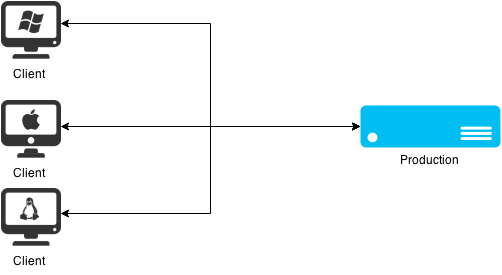
\includegraphics[scale=0.36]{02_2015_01_example}
\end{figure}


Имеется некое клиент"=серверное приложение, и периодически возникает задача его обновлять. При обновлениях возникает время простоя, пользователи выражают недовольство и перестают пользоваться данным приложением (заходить на сайт, оставлять заявки с службу технической поддержки и т.~п.).

Первым этапом в улучшении приложения стала модификация сетевой инфраструктуры "--- добавился сервер для тестирования обновлений, так называемый \emph{staging"=сервер}:

~

\begin{figure}[h!]
  \centering
  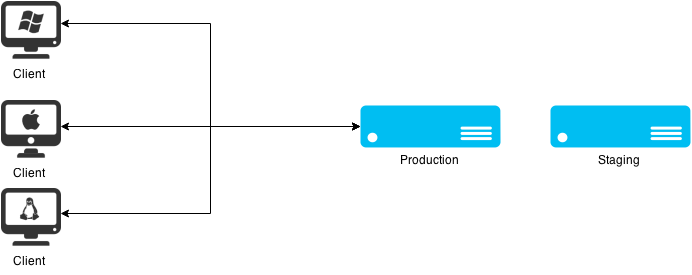
\includegraphics[scale=0.36]{02_2015_02_staging}
\end{figure}

Стало лучше, возможность успешной установки обновлений предварительно проверялась, проверялась и работоспособность основных функций приложения после обновления. Время простоя уменьшилось (как и недовольство пользователей), но не исчезло.

Следующим этапом в улучшении стало добавление обратного прокси в структуру приложения:

~

\begin{figure}[h!]
  \centering
  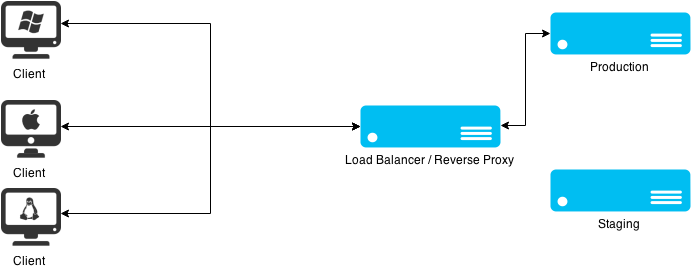
\includegraphics[scale=0.36]{02_2015_03_working}
\end{figure}

Данная структура обеспечила возможность горизонтального масштабирования системы и позволила гибко переключаться между серверами при необходимости (ликвидировать простои на время обслуживания).


Изначально было решено поступить следующим образом: при подготовке сервера к обновлению происходит синхронизация данных на staging"=сервер, затем на нем происходит обновление приложения и основная проверка работоспособности:


\begin{figure}[h!]
  \centering
  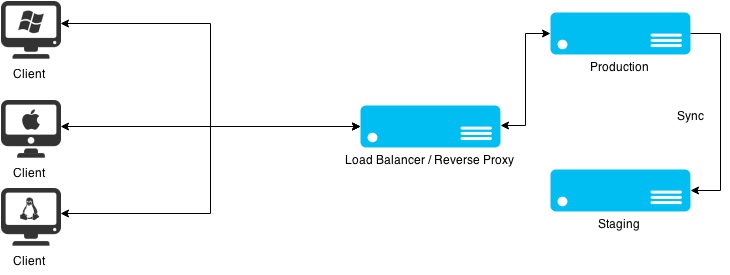
\includegraphics[scale=0.35]{02_2015_04_sync_to_stage}
\end{figure}

Затем происходит переключение обратного прокси на staging"=сервер, переключение длится несколько секунд (из серьезных недостатков "--- мы теряем все активные сессии пользователей). В остальном "--- для конечного пользователя вообще ничего не меняется.

\begin{figure}[h!]
  \centering
  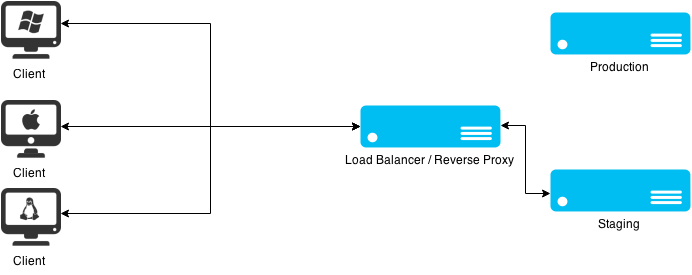
\includegraphics[scale=0.35]{02_2015_05_work_on_stage}
\end{figure}

После переключения нагрузки на staging"=сервер, на \emph{production"=сервере} обновляется приложение. После успешного обновления и проверки его жизнеспособности начинается синхронизация данных со staging (теоретически конечные пользователи уже внесли изменения в данных приложения).

\begin{figure}[h!]
  \centering
  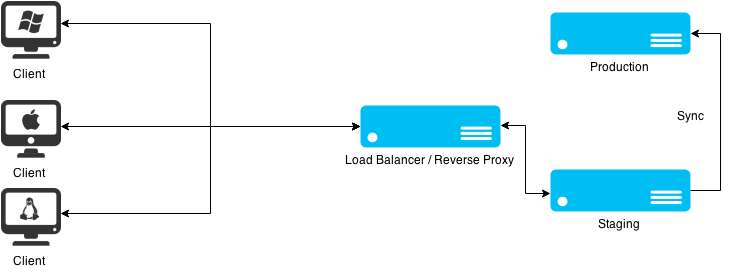
\includegraphics[scale=0.35]{02_2015_06_sync_to_prod}
\end{figure}

После окончания синхронизации происходит переключение обратного прокси"=сервера обратно на production"=сервер.

\begin{figure}[h!]
  \centering
  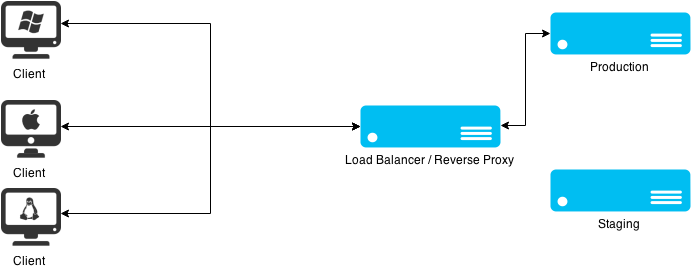
\includegraphics[scale=0.36]{02_2015_07_working_on_prod}
\end{figure}

Но при тестировании на реальных данных нашелся небольшой процент пользователей который изменял данные в момент после синхронизации данных и до переключения между серверами.
В связи с этим, было решено изменить механизм работы приложения.

Был разработан механизм, переводивший приложение в режим <<только чтение>> и уведомлявший пользователей. Перед обновлением production"=сервер переводился в режим <<только чтение>>.

\begin{figure}[h!]
  \centering
  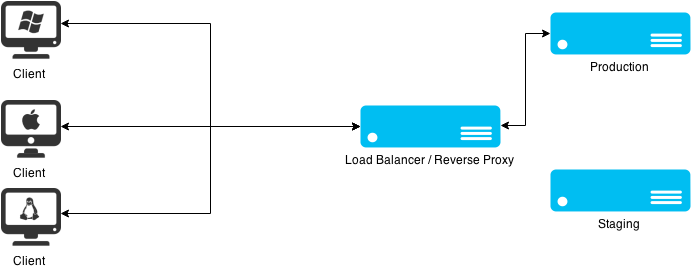
\includegraphics[scale=0.36]{02_2015_08_working}
\end{figure}

После этого происходила синхронизация на staging"=сервер. Приложение на staging"=сервере также в режиме <<только чтение>>.

\begin{figure}[h!]
  \centering
  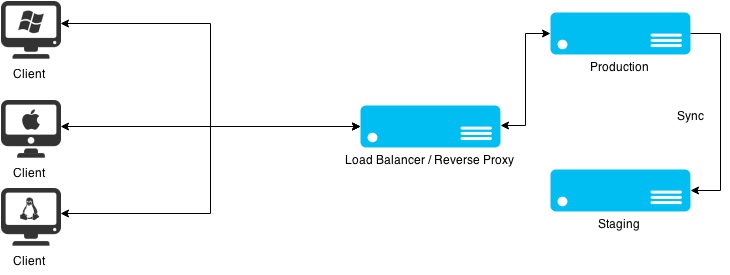
\includegraphics[scale=0.36]{02_2015_09_sync_to_stage}
\end{figure}

После этих манипуляций происходит переключение production"=прокси на staging, и при этом мы убрали вероятность потери данных в момент синхронизации"=переключения. Пользователи получили доступ к приложению и его данным только на чтение на момент обновления, количество негативных отзывов стало минимальным за все время (все отнеслись с пониманием к надписи, предупреждающей о технических работах). Далее "--- переключение приложения на staging, обновление production"=сервера, переключение обратно, и лишь затем "--- отключение режима <<только чтение>>.

\begin{figure}[h!]
  \centering
  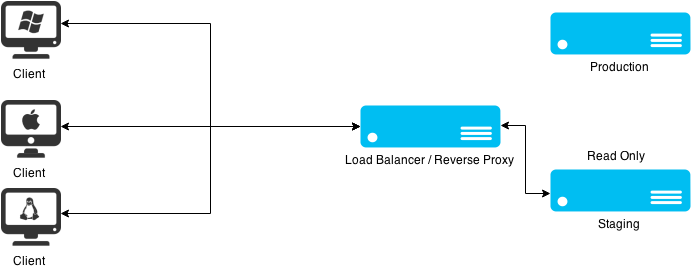
\includegraphics[scale=0.36]{02_2015_10_readonly_work_on_stage}
\end{figure}

\subsection*{Вместо заключения}

Мы добились высокой доступности приложения. При этом, синхронизация данных максимально упрощена, необходимости в изменении работы логики приложения нет (что в свою очередь позволяет ее применять к уже существующим решениям без добавления / изменения логики работы).

\end{document}

\documentclass[10pt, a5paper]{article}
\usepackage{pdfpages}
\usepackage{parallel}
\usepackage[T2A]{fontenc}
\usepackage{ucs}
\usepackage[utf8x]{inputenc}
\usepackage[polish,english,russian]{babel}
\usepackage{hyperref}
\usepackage{rotating}
\usepackage[inner=2cm,top=1.8cm,outer=2cm,bottom=2.3cm,nohead]{geometry}
\usepackage{listings}
\usepackage{graphicx}
\usepackage{wrapfig}
\usepackage{longtable}
\usepackage{indentfirst}
\usepackage{array}
\newcolumntype{P}[1]{>{\raggedright\arraybackslash}p{#1}}
\frenchspacing
\usepackage{fixltx2e} %text sub- and superscripts
\usepackage{icomma} % коскі ў матэматычным рэжыме
\PreloadUnicodePage{4}

\newcommand{\longpage}{\enlargethispage{\baselineskip}}
\newcommand{\shortpage}{\enlargethispage{-\baselineskip}}

\def\switchlang#1{\expandafter\csname switchlang#1\endcsname}
\def\switchlangbe{
\let\saverefname=\refname%
\def\refname{Літаратура}%
\def\figurename{Іл.}%
}
\def\switchlangen{
\let\saverefname=\refname%
\def\refname{References}%
\def\figurename{Fig.}%
}
\def\switchlangru{
\let\saverefname=\refname%
\let\savefigurename=\figurename%
\def\refname{Литература}%
\def\figurename{Рис.}%
}

\hyphenation{admi-ni-stra-tive}
\hyphenation{ex-pe-ri-ence}
\hyphenation{fle-xi-bi-li-ty}
\hyphenation{Py-thon}
\hyphenation{ma-the-ma-ti-cal}
\hyphenation{re-ported}
\hyphenation{imp-le-menta-tions}
\hyphenation{pro-vides}
\hyphenation{en-gi-neering}
\hyphenation{com-pa-ti-bi-li-ty}
\hyphenation{im-pos-sible}
\hyphenation{desk-top}
\hyphenation{elec-tro-nic}
\hyphenation{com-pa-ny}
\hyphenation{de-ve-lop-ment}
\hyphenation{de-ve-loping}
\hyphenation{de-ve-lop}
\hyphenation{da-ta-ba-se}
\hyphenation{plat-forms}
\hyphenation{or-ga-ni-za-tion}
\hyphenation{pro-gramming}
\hyphenation{in-stru-ments}
\hyphenation{Li-nux}
\hyphenation{sour-ce}
\hyphenation{en-vi-ron-ment}
\hyphenation{Te-le-pathy}
\hyphenation{Li-nux-ov-ka}
\hyphenation{Open-BSD}
\hyphenation{Free-BSD}
\hyphenation{men-ti-on-ed}
\hyphenation{app-li-ca-tion}

\def\progref!#1!{\texttt{#1}}
\renewcommand{\arraystretch}{2} %Іначай формулы ў матрыцы зліпаюцца з лініямі
\usepackage{array}

\def\interview #1 (#2), #3, #4, #5\par{

\section[#1, #3, #4]{#1 -- #3, #4}
\def\qname{LVEE}
\def\aname{#1}
\def\q ##1\par{{\noindent \bf \qname: ##1 }\par}
\def\a{{\noindent \bf \aname: } \def\qname{L}\def\aname{#2}}
}

\def\interview* #1 (#2), #3, #4, #5\par{

\section*{#1\\{\small\rm #3, #4. #5}}

\def\qname{LVEE}
\def\aname{#1}
\def\q ##1\par{{\noindent \bf \qname: ##1 }\par}
\def\a{{\noindent \bf \aname: } \def\qname{L}\def\aname{#2}}
}

\begin{document}
\title{Параўнальны аналіз сродкаў кросплатформеннага праграмавання}
\author{Г. Злобін, А. Чмихало, Львів, Украіна\footnote{\url{zlobingg@gmail.com}, \url{http://lvee.org/en/abstracts/148}}}
\maketitle
\begin{abstract}
The article provides a comparative analysis of crossplatform programming tools. Crossplatform programming tools are divided into three groups: crossplatform compiled languages (Table 1), crossplatform programming languages at the execution level \linebreak (Table 2) and crossplatform interpreters (Table 3). The informa\-tion in Tables 1--3 is ordered by number of supported operating systems (descending). Table 4 provides information about \linebreak standardized libraries and frameworks used in crossplatform programming. To substantiate the analysis results, the index of popularity of programming languages ​​TIOBE is used.
\end{abstract}
Кросплатформеннасць "--- гэта здольнасць праграмнага забеспячэння працаваць больш чым на адной платформе або аперацыйнай сістэме. Кросплатформннасць праграмнага забеспячэння набыла асаблівае значэнне пасля завяршэння эры практычна непадзельнага панавання платформы Wintel (x86 + Microsoft Windows). Як вынікае з [1],   колькасць працоўных месцаў з не"=Wintel платформай у 2012 перавысіла 65\% і працягвае павялічвацца. Гэта зрабіла эканамічна прывабным кросплатформеннае праграмаванне ў галіне распрацоўкі прыкладнога праграмнага забеспячэння.

Мовы праграмавання, якія можна выкарыстоўваць для крос\-платформеннай распрацоўкі праграм, дзеляцца на тры групы:

\begin{itemize}
  \item кросплатформавыя мовы праграмавання на ўзроўні кампіляцыі "--- для гэтых моў існуюць кампілятары для розных платформаў (C, C++, Pascal, Fortran, Ада і г.д.);
  \item кросплатформавыя мовы на ўзроўні выканання (Java і C\#) "--- вынікам працы кампілятара ў гэтых мовах ёсць байт"=код, які можна запускаць на розных платформах з дапамогай віртуальных машын (Java VM для Java і CLR для C\#);
  \item кросплатформавыя інтэрпрэтатары "--- для гэтых моў \linebreak з'яўляюцца інтэрпрэтатары (PHP, Perl, Python, Tcl, Ruby і т.д.) для розных платформаў.
\end{itemize}

\begin{table}
\label{z_table1}
\caption{~}
	\centering
  \begin{tabular}{ p{1.6cm} p{4.6cm} p {3.6cm} }
\hline
    Інструмен\-тальная абалонка & Падтрымліваюцца кампілятары/колькасць моў праграмавання & Падтрымліваюцца АС / іх колькасць \\ \hline
    Qt Creator  & GCC, Clang, MinGW, MSVC, Linux ICC, GCCE, RVCT, WINSCW / 8  & Linux, OS X, Windows, Unix,  iOS, Android, Blackberry 10, WinRT, Embed. Linux, QNX / 10  \\
    Eclipse  & C/С++, Fortran/3  & AIX, FreeBSD, HP-UX, Linux, Mac OS X, OpenSolaris, Solaris, QNX, Windows, Android (AR) / 10 \\
    Free Pascal  & Free Pascal Compiler, Object Pascal, част. GNU Pascal, ISO Extended Pascal / 4  & DOS, FreeBSD, Linux, Mac OS X, Windows, Sun Solaris, Haiku / 7  \\
    Lazarus & Free Pascal Compiler / 1 & Linux, FreeBSD, Mac OS X, Windows, Android / 5  \\
    Code:: Blocks  & MinGW,~GCC~C/C++,~GNU GCC~(PowerPC,~ARM,~AVR), SDCC, Digital Mars (C/C++, D), Visual C++, Borland C++, Watcom, Intel C++, GNU Fortran, GNU ARM, GNU GDC / 15  & Windows, Linux, Mac OS X, Unix / 4 \\
    NetBeans IDE & C, C++, Ада / 3  & Windows, Linux, ~~ FreeBSD,  Solaris / 4  \\
    Embarcade\-ro~RAD~Stu\-dio XE7 & Delphi, С, C++ / 3 & Windows, Mac OS X, iOS, Android / 4  \\ \hline
  \end{tabular}
\end{table}

Разгледзім кароткія характарыстыкі кросплатформавых моў \linebreak праграмавання на ўзроўні кампіляцыі ў таблiцы 1.

\begin{table}
\label{z_table2}
\caption{~}
	\centering
  \begin{tabular}{ p{2cm} p {3.5cm} p{4cm} }
\hline
    Інстру\-ментальная абалонка & Падтрымліваюцца кампілятары/колькасць моў праграмавання & Падтрымліваюцца АС / іх колькасць \\ \hline
    Eclipse\footnotemark[1] & Java & AIX, FreeBSD, HP-UX, Linux, Mac OS X, OpenSolaris, Solaris, QNX, Microsoft Windows, Android (ARM) / 10  \\
    NetBeans IDE\footnotemark[1] & Java & Windows, Linux, FreeBSD,  Solaris / 4  \\
    IntelliJ IDEA\footnotemark[1] & Java & Linux, Mac OS X,  Windows / 3  \\
    AIDE\footnotemark[1] & Java &  Android \\
    Microsoft Visual Studio Code & C\#, Java/2 & Linux, Mac OS X / 2 \\
    .NET Core 5 & C\# &  Linux, Mac OS X / 2 \\
    Mono & C\# & Linux, MacOS / 2  \\
\hline
  \end{tabular}
\end{table}


У табліцы 2 прадстаўлены кароткія характарыстыкі  кросплатформавых моў  на ўзроўні  выканання\footnote{Праз вялікую колькасць інструментальных сродкаў для Java іх пералік няпоўны}.


У табліцы 3 прадстаўлены кароткія характарыстыкі  кросплатформавых інтэрпрэтатараў.

\begin{table}
\label{z_table3}  
\caption{~}
	\centering
  \begin{tabular}{ p{2cm} p {3.5cm} p{4cm} }
    \hline
    Інстру\-ментальная абаолонка & Падтрымліваюцца кампілятары~/ колькасць моў праграмавання & Падтрымліваюцца АС / іх колькасць \\ \hline
    Eclipse & Perl, PHP, JavaScript, Python, Ruby/5 & AIX, FreeBSD, HP-UX, Linux, Mac OS X, OpenSolaris, Solaris, QNX, Microsoft Windows, Android (ARM) / 10  \\
    NetBeans IDE & Java, JavaFX, PHP, JavaScript, HTML5, Python, Groovy / 7 & Windows, Linux, FreeBSD,  Solaris / 4  \\
    Embarcadero RAD Studio XE7 & HTML5 & Windows, Mac OS X, iOS, Android / 4  \\
    Xojo IDE Real  & Basic & OS X, Windows, Linux, iOS / 4  \\
    Komodo IDE/Komodo Edit & Perl, PHP, Python, Ruby, Tcl. JavaScript, CSS3, HTML5, XML,  XSLT / 10 & Linux, Mac OS X, Windows / 3  \\
    PyCharm & Python, JavaScript, HTML / 3 &  Windows, Linux, Mac OS X / 3 \\
    Aptana Studio 3 & JavaScript, PHP, Ruby, Python / 4 & Windows, Linux, Mac OS X / 3  \\
    Microsoft Visual Studio Code & Python, JavaScript, PHP, JSON, XML, HTML, CSS / 7 & Mac OS X, Linux / 2  \\ \hline
  \end{tabular}
\end{table}
На жаль, аўтарам невядомыя даследаванні папулярнасці сродкаў кросплатформеннага праграмавання, таму скарыстаемся індэксам TIOBE [2], па якім ацэньваюць папулярнасць моў праграмавання. Як вынікае з [2], найбольшай папулярнасцю больш за 10 гадоў карыстаюцца мовы праграмавання C (на 1.2015 г. 16,703\%) і Java (15,528\%), якія шырока выкарыстоўваюць для кросплатформеннага праграмавання. Менш папулярныя C++ (6,705\%), C\# (5,045\%), PHP (3,784\%), Python (2,613\%), Perl (2,256\%), Delphi / Object Pascal (0,837\%). Яшчэ адным фактарам адбору можа быць колькасць аперацыйных сістэм і колькасць апаратных платформаў, для якіх можна выкарыстоўваць сродкі кросплатформеннага распрацоўкі. Не менш важнымі для кросплатформеннага праграмавання з'яўляецца стандартызаваныя бібліятэкі часу выканання. У прыватнасці, стандартам стала бібліятэка мовы Сі. Cвои стандартныя бібліятэкі маюць C++, Java, Python, Ruby, якія падаюцца разам са сродкамі распрацоўкі і даступныя на падтрымоўваных платформах. Варта адзначыць таксама некаторыя вялікія кросплатформавыя бібліятэкі "--- такія як Qt, GTK+, FLTK, STL, Boost, OpenGL, SDL, OpenAL, OpenCL. У табліцы 4 стандартныя бібліятэкі часу выканання падзеленыя на бібліятэкі з адкрытым кодам і бібліятэкі з зачыненым кодам.

\begin{table}
\caption{Стандартныя бібліятэкі і праграмныя каркасы з адкрытым і зачыненым кодам}
\label{z_table4}
  \centering
  \begin{tabular}{p{6cm} p{3.5cm}}
     \hline
    Бібліятэкі і праграмныя каркасы з адкрытым кодам / адкрытыя стандарты & Бібліятэкі і праграмныя каркасы з зачыненым кодам \\ \hline
    Boost, GIMP ToolKit, GTK+, FLTK, Kivy, OpenCV, OpenCL, OpenGL, SDL, Apache Cordova,  Tk &  \\
    OpenAL (раннія версіі) & OpenAL (пазнейшыя версіі) \\
    Qt & Qt \\
    Simple DirectMedia Layer & Unity3D \\ \hline
  \end{tabular}
\end{table}
\subsection*{Высновы}

\begin{enumerate}
  \item Па папулярнасці моў праграмавання сярод кампілятараў першае месца займае мова праграмавання C, сярод інтэрпрэтатараў "--- мова Java.
  \item Па індэксе Tiobe ў студзені 2015 мова праграмавання Delpi / Object Pascal займае 20 месца.
  \item ППа колькасці аперацыйных сістэм, у якіх можна скарыстацца згаданымі ў аглядзе сродкамі распрацоўкі, яны размешчаны ў табліцах 1--3. Апошняя радок у табліцы 1 (кросплатформеннага мовы праграмавання на ўзроўні кампіляцыі) з двума падтрымоўванымі АС займае Microsoft Visual Studio Code, ў табліцы 2 (кросплатформенныя мовы праграмавання на ўзроўні выканання) тры апошнія радкі з двума падтрыманымі АС займаюць Microsoft Visual Studio Code, .NET Core 5, Mono, у табліцы 3 (кросплатформавыя інтэрпрэтатары) апошнi радок з двума падтрыманымі АС займае Microsoft Visual Studio Code.
  \item Як і варта было чакаць колькасць стандартных бібліятэк з адкрытым кодам амаль у чатыры разы перавышае колькасць стандартных бібліятэк з зачыненым кодам.
\end{enumerate}

\section*{Iнфармацыйныя сродкi}

\begin{enumerate}
\item D. Thompson. The 11 Most Fascinating Charts From Mary Meeker's Epic Slideshow of Internet Trends. \url{http://tinyurl.com/ozwck2k}
\item TIOBE Index for May 2015. \url{http://www.tiobe.com/index.php/content/paperinfo/tpci/index.html} \end{enumerate}
\end{document}

\documentclass[10pt, a5paper]{article}
\usepackage{pdfpages}
\usepackage{parallel}
\usepackage[T2A]{fontenc}
\usepackage{ucs}
\usepackage[utf8x]{inputenc}
\usepackage[polish,english,russian]{babel}
\usepackage{hyperref}
\usepackage{rotating}
\usepackage[inner=2cm,top=1.8cm,outer=2cm,bottom=2.3cm,nohead]{geometry}
\usepackage{listings}
\usepackage{graphicx}
\usepackage{wrapfig}
\usepackage{longtable}
\usepackage{indentfirst}
\usepackage{array}
\newcolumntype{P}[1]{>{\raggedright\arraybackslash}p{#1}}
\frenchspacing
\usepackage{fixltx2e} %text sub- and superscripts
\usepackage{icomma} % коскі ў матэматычным рэжыме
\PreloadUnicodePage{4}

\newcommand{\longpage}{\enlargethispage{\baselineskip}}
\newcommand{\shortpage}{\enlargethispage{-\baselineskip}}

\def\switchlang#1{\expandafter\csname switchlang#1\endcsname}
\def\switchlangbe{
\let\saverefname=\refname%
\def\refname{Літаратура}%
\def\figurename{Іл.}%
}
\def\switchlangen{
\let\saverefname=\refname%
\def\refname{References}%
\def\figurename{Fig.}%
}
\def\switchlangru{
\let\saverefname=\refname%
\let\savefigurename=\figurename%
\def\refname{Литература}%
\def\figurename{Рис.}%
}

\hyphenation{admi-ni-stra-tive}
\hyphenation{ex-pe-ri-ence}
\hyphenation{fle-xi-bi-li-ty}
\hyphenation{Py-thon}
\hyphenation{ma-the-ma-ti-cal}
\hyphenation{re-ported}
\hyphenation{imp-le-menta-tions}
\hyphenation{pro-vides}
\hyphenation{en-gi-neering}
\hyphenation{com-pa-ti-bi-li-ty}
\hyphenation{im-pos-sible}
\hyphenation{desk-top}
\hyphenation{elec-tro-nic}
\hyphenation{com-pa-ny}
\hyphenation{de-ve-lop-ment}
\hyphenation{de-ve-loping}
\hyphenation{de-ve-lop}
\hyphenation{da-ta-ba-se}
\hyphenation{plat-forms}
\hyphenation{or-ga-ni-za-tion}
\hyphenation{pro-gramming}
\hyphenation{in-stru-ments}
\hyphenation{Li-nux}
\hyphenation{sour-ce}
\hyphenation{en-vi-ron-ment}
\hyphenation{Te-le-pathy}
\hyphenation{Li-nux-ov-ka}
\hyphenation{Open-BSD}
\hyphenation{Free-BSD}
\hyphenation{men-ti-on-ed}
\hyphenation{app-li-ca-tion}

\def\progref!#1!{\texttt{#1}}
\renewcommand{\arraystretch}{2} %Іначай формулы ў матрыцы зліпаюцца з лініямі
\usepackage{array}

\def\interview #1 (#2), #3, #4, #5\par{

\section[#1, #3, #4]{#1 -- #3, #4}
\def\qname{LVEE}
\def\aname{#1}
\def\q ##1\par{{\noindent \bf \qname: ##1 }\par}
\def\a{{\noindent \bf \aname: } \def\qname{L}\def\aname{#2}}
}

\def\interview* #1 (#2), #3, #4, #5\par{

\section*{#1\\{\small\rm #3, #4. #5}}

\def\qname{LVEE}
\def\aname{#1}
\def\q ##1\par{{\noindent \bf \qname: ##1 }\par}
\def\a{{\noindent \bf \aname: } \def\qname{L}\def\aname{#2}}
}

\begin{document}
\title{О том как маленький opensource"=проект меняет жизнь большой компании}
\author{Павел Емельянов, Москва, РФ\footnote{\url{xemul@openvz.org}, \url{http://lvee.org/en/abstracts/149}}}
\maketitle
\begin{abstract}
CRIU is the open source checkpoint"=restore project of the Odin (former Parallels) company. It provides basis for containers live migration, seamless kernel update and a set of other features. In this talk I will present the current state of the project, describe the community that has grown around it and show how the open development model of a small project affected the life of the whole company.
\end{abstract}
OpenVZ "--- это открытый проект компании Odin, дающий пользователям простую, но надёжную контейнерную платформу. Неотъемлемой частью проекта с самого его начала является возможность живой миграции контейнеров, для чего используется технология <<снятия контрольных точек>> (checkpoint) и восстановления из них (restore). В процессе продвижения контейнерной технологии в массы инженеры компании были вынуждены переписать C/R подсистему практически с нуля и в другой парадигме "--- вместо ядерного модуля checkpoint"=restore теперь делается силами процесса с использованием открытых ядерных интерфейсов. Вместе со сменой <<адресного пространства>> кода был изменён и подход к разработке "--- CRIU это 100\% открытый проект без скрытых компонент и без диктатуры инженеров Odin при принятии архитектурных и технических решений.

За 4 года своего существования CRIU разросся до 100 тысяч строк кода и, что ещё важнее, достиг определённых успехов в социальной сфере.

Во"=первых, проект завоевал признание в сообществе Linux kernel, куда изначально предлагалась реализация технологии, и теперь достаточным поводом для начала обсуждения ядерных патчей может служить простая фраза: <<это надо для CRIU>>.

Во"=вторых, CRIU <<подружился>> с другими проектами, например Docker и LXC, так что теперь идеи и улучшения мы получаем не только от клиентов Odin"=а.

В"=третьих, CRIU оброс небольшим сообществом, которое уже принесло свои плоды "--- портирование на архитектуры AArch64 и Power, интеграция с LXC и Docker и много другого было сделано не нами, но и для нас в том числе.

И, наконец, проект оказал сильное влияние на весь процесс разработки компании Odin. Недавно начатая новая жизнь OpenVZ планировалась с учетом приобретённого в CRIU опыта ведения открытых проектов.

\end{document}

\documentclass[10pt, a5paper]{article}
\usepackage{pdfpages}
\usepackage{parallel}
\usepackage[T2A]{fontenc}
\usepackage{ucs}
\usepackage[utf8x]{inputenc}
\usepackage[polish,english,russian]{babel}
\usepackage{hyperref}
\usepackage{rotating}
\usepackage[inner=2cm,top=1.8cm,outer=2cm,bottom=2.3cm,nohead]{geometry}
\usepackage{listings}
\usepackage{graphicx}
\usepackage{wrapfig}
\usepackage{longtable}
\usepackage{indentfirst}
\usepackage{array}
\newcolumntype{P}[1]{>{\raggedright\arraybackslash}p{#1}}
\frenchspacing
\usepackage{fixltx2e} %text sub- and superscripts
\usepackage{icomma} % коскі ў матэматычным рэжыме
\PreloadUnicodePage{4}

\newcommand{\longpage}{\enlargethispage{\baselineskip}}
\newcommand{\shortpage}{\enlargethispage{-\baselineskip}}

\def\switchlang#1{\expandafter\csname switchlang#1\endcsname}
\def\switchlangbe{
\let\saverefname=\refname%
\def\refname{Літаратура}%
\def\figurename{Іл.}%
}
\def\switchlangen{
\let\saverefname=\refname%
\def\refname{References}%
\def\figurename{Fig.}%
}
\def\switchlangru{
\let\saverefname=\refname%
\let\savefigurename=\figurename%
\def\refname{Литература}%
\def\figurename{Рис.}%
}

\hyphenation{admi-ni-stra-tive}
\hyphenation{ex-pe-ri-ence}
\hyphenation{fle-xi-bi-li-ty}
\hyphenation{Py-thon}
\hyphenation{ma-the-ma-ti-cal}
\hyphenation{re-ported}
\hyphenation{imp-le-menta-tions}
\hyphenation{pro-vides}
\hyphenation{en-gi-neering}
\hyphenation{com-pa-ti-bi-li-ty}
\hyphenation{im-pos-sible}
\hyphenation{desk-top}
\hyphenation{elec-tro-nic}
\hyphenation{com-pa-ny}
\hyphenation{de-ve-lop-ment}
\hyphenation{de-ve-loping}
\hyphenation{de-ve-lop}
\hyphenation{da-ta-ba-se}
\hyphenation{plat-forms}
\hyphenation{or-ga-ni-za-tion}
\hyphenation{pro-gramming}
\hyphenation{in-stru-ments}
\hyphenation{Li-nux}
\hyphenation{sour-ce}
\hyphenation{en-vi-ron-ment}
\hyphenation{Te-le-pathy}
\hyphenation{Li-nux-ov-ka}
\hyphenation{Open-BSD}
\hyphenation{Free-BSD}
\hyphenation{men-ti-on-ed}
\hyphenation{app-li-ca-tion}

\def\progref!#1!{\texttt{#1}}
\renewcommand{\arraystretch}{2} %Іначай формулы ў матрыцы зліпаюцца з лініямі
\usepackage{array}

\def\interview #1 (#2), #3, #4, #5\par{

\section[#1, #3, #4]{#1 -- #3, #4}
\def\qname{LVEE}
\def\aname{#1}
\def\q ##1\par{{\noindent \bf \qname: ##1 }\par}
\def\a{{\noindent \bf \aname: } \def\qname{L}\def\aname{#2}}
}

\def\interview* #1 (#2), #3, #4, #5\par{

\section*{#1\\{\small\rm #3, #4. #5}}

\def\qname{LVEE}
\def\aname{#1}
\def\q ##1\par{{\noindent \bf \qname: ##1 }\par}
\def\a{{\noindent \bf \aname: } \def\qname{L}\def\aname{#2}}
}

\begin{document}
\title{Рекурсивное наблюдение за файловой системой на примере librnotify}
\author{Андрей Змушко, Минск, Беларусь\footnote{\url{andrey.zmushko@gmail.com}, \url{http://lvee.org/en/abstracts/152}}}
\maketitle
\begin{abstract}
One of base questions that appear in data synchronisation, is getting file notifications from the directory. Common solution for this is using a Linux kernel subsystem such as inotify or fanotify. Since fanotify doesn't notify file deletions, file renames or file moves, it is difficult to use fanotify for such applications. But of course fanotify gives as pid of process which have caused the event to happen. This can be very useful for some special cases, for example we should ignore events created by themselves. But in synchronisation it is very important to provide good support of move folders, in fact it is common problem for most synchronisation apps. In this subject we will review inotify just deeper. Known problems of inotify are that it provides no way of recursive monitoring and no map between watch descriptor and real path. Both thess questions have been solved in librnotify. 
\end{abstract}
Предположим, стоит задача синхронизировать данные, хранящиеся в некоторых директориях, доступ к которым не ограничен. Очевидно, что мы будем вынуждены периодически рекурсивно просматривать директорию, чтобы находить различия или подписаться на файловые нотификации, которые поставляются такими подсистемами ядра Linux, как inotify и fanotify.

fanotify имеет серьезный недостаток: не поддерживаются нотификации удаления и перемещения. 
Поэтому применение его в синхронизации данных усложняется. 

Рассмотрим inotify. Основных недостатков в нем, пожалуй, три: первый "--- это то, что нотификация сопровождается только лишь  
дескриптором, и ничего не известно о пути сработавшего элемента ФС, если об этом не позаботиться заранее. 

Второй "--- это ограничения (лимиты) 
в ядре на количество запущенных нотификаторов и длину очереди нотификаций. Лимиты можно и нужно менять, и скорее ваше приложение упрется в ограничения, связанные с производительностью, чем в лимит.  

И последний недостаток "--- это то, что совсем не поддерживается рекурсивная нотификация папок.  
То есть когда, допустим, мы перемещаем папку внутрь нотифицируемой папки, пока интерфейс просигнализирует о новой папке и мы включим эту новую папку в нотификации, 
 несколько файлов <<проскочат>> мимо, и мы получим рассинхронизацию данных; это случается практически постоянно. 
Одним из известных решений по устранению этой проблемы является проект lsync. Действительно, он полностью решает две проблемы: маппинг путей и рекурсивные нотификации. Но он громоздок и непроизводителен в качестве подсистемы. 

В одном из наших проектов мы использовали lsync как сервер нотификаций, но если нужно синхронизировать десяток разных корневых папок с сотнями тысяч файлов и папок внутри, решение с lsinc
оказывается дорогим в плане потребления системных ресурсов. 
В итоге мы заменили lsync на библиотеку librnotify. 

Подробно опишем интерфейс этой библиотеки. 
Он прост и содержит только три вызова: 
\begin{verbatim}
Notify* initNotify(const char* path, const uint32_t mask,
                   const char* exclude); 
int waitNotify(Notify* ntf, char** const path, uint32_t*
               mask, const int timeout, uint32_t* cookie); 
void freeNotify(Notify* ntf);
\end{verbatim}

Объект Notify является контейнером состояния нотификатора, и с нашей точки зрения нам не интересен. 
initNotify подписывает некую папку по пути path на список нотификаций, задаваемый в mask (список тот же, что и в man inotify). Естественно, файл \linebreak sys/inotify.h также должен присутствовать. exclude "--- это регулярное выражение, которое задает маску для элементов ФС, которые мы не хотим нотифицировать "--- это удобно, если, например, мы не хотим нотифицировать .git или просто .*.

Вызов waitNotify ждет нотификации timeout секунд (или микросекунд), а при значении 0 ждет вечно. Он возвращает path и битовое поле (mask), где указанно, что именно случилось. 
Cookie "--- это возвращаемое число, которое позволяет связать нотификации перемещения; оно будет одинаковым для пар операций MOVE\_FROM и MOVE\_TO. 
Наконец, freeNotify удаляет объект нотификатора.

Библиотека librnotify доступна по адресу \url{https://github.com/zmushko/librnotify}

\end{document}

\documentclass[10pt, a5paper]{article}
\usepackage{pdfpages}
\usepackage{parallel}
\usepackage[T2A]{fontenc}
\usepackage{ucs}
\usepackage[utf8x]{inputenc}
\usepackage[polish,english,russian]{babel}
\usepackage{hyperref}
\usepackage{rotating}
\usepackage[inner=2cm,top=1.8cm,outer=2cm,bottom=2.3cm,nohead]{geometry}
\usepackage{listings}
\usepackage{graphicx}
\usepackage{wrapfig}
\usepackage{longtable}
\usepackage{indentfirst}
\usepackage{array}
\newcolumntype{P}[1]{>{\raggedright\arraybackslash}p{#1}}
\frenchspacing
\usepackage{fixltx2e} %text sub- and superscripts
\usepackage{icomma} % коскі ў матэматычным рэжыме
\PreloadUnicodePage{4}

\newcommand{\longpage}{\enlargethispage{\baselineskip}}
\newcommand{\shortpage}{\enlargethispage{-\baselineskip}}

\def\switchlang#1{\expandafter\csname switchlang#1\endcsname}
\def\switchlangbe{
\let\saverefname=\refname%
\def\refname{Літаратура}%
\def\figurename{Іл.}%
}
\def\switchlangen{
\let\saverefname=\refname%
\def\refname{References}%
\def\figurename{Fig.}%
}
\def\switchlangru{
\let\saverefname=\refname%
\let\savefigurename=\figurename%
\def\refname{Литература}%
\def\figurename{Рис.}%
}

\hyphenation{admi-ni-stra-tive}
\hyphenation{ex-pe-ri-ence}
\hyphenation{fle-xi-bi-li-ty}
\hyphenation{Py-thon}
\hyphenation{ma-the-ma-ti-cal}
\hyphenation{re-ported}
\hyphenation{imp-le-menta-tions}
\hyphenation{pro-vides}
\hyphenation{en-gi-neering}
\hyphenation{com-pa-ti-bi-li-ty}
\hyphenation{im-pos-sible}
\hyphenation{desk-top}
\hyphenation{elec-tro-nic}
\hyphenation{com-pa-ny}
\hyphenation{de-ve-lop-ment}
\hyphenation{de-ve-loping}
\hyphenation{de-ve-lop}
\hyphenation{da-ta-ba-se}
\hyphenation{plat-forms}
\hyphenation{or-ga-ni-za-tion}
\hyphenation{pro-gramming}
\hyphenation{in-stru-ments}
\hyphenation{Li-nux}
\hyphenation{sour-ce}
\hyphenation{en-vi-ron-ment}
\hyphenation{Te-le-pathy}
\hyphenation{Li-nux-ov-ka}
\hyphenation{Open-BSD}
\hyphenation{Free-BSD}
\hyphenation{men-ti-on-ed}
\hyphenation{app-li-ca-tion}

\def\progref!#1!{\texttt{#1}}
\renewcommand{\arraystretch}{2} %Іначай формулы ў матрыцы зліпаюцца з лініямі
\usepackage{array}

\def\interview #1 (#2), #3, #4, #5\par{

\section[#1, #3, #4]{#1 -- #3, #4}
\def\qname{LVEE}
\def\aname{#1}
\def\q ##1\par{{\noindent \bf \qname: ##1 }\par}
\def\a{{\noindent \bf \aname: } \def\qname{L}\def\aname{#2}}
}

\def\interview* #1 (#2), #3, #4, #5\par{

\section*{#1\\{\small\rm #3, #4. #5}}

\def\qname{LVEE}
\def\aname{#1}
\def\q ##1\par{{\noindent \bf \qname: ##1 }\par}
\def\a{{\noindent \bf \aname: } \def\qname{L}\def\aname{#2}}
}

\begin{document}
\title{Программирование на C для PostgreSQL}
\author{Александр Коротков, Москва, РФ\footnote{\url{aekorotkov@gmail.com}, \url{http://lvee.org/en/abstracts/153}}}
\maketitle
\begin{abstract}
PostgreSQL offers great extendability. Users can add literally everything on their own: data types, functions, operators, index types, procedural languages and so on. But in order to use the full power of these features one should write C code for \linebreak PostgreSQL. Traditionally it's assumed that barrier to entry of C programming for PostgreSQL is very high. That's why extendability of PostgreSQL is no as demanded as it could be. The goal of present talk is to overcome this circumstances.
\end{abstract}
PostgreSQL обладает отличной расширяемостью, пользователи могут добавлять сами буквально всё: типы данных, функции, операторы, типы индексов, языки хранимых процедур и т.д. Но для того, чтобы использовать многие из этих возможностей, нужно уметь программировать под PostgreSQL на C.

Традиционно считается, что это сложно и порог вхождения \linebreak очень велик. Из"=за этого вся мощь расширяемости PostgreSQL оказывается не так востребована, как могла бы быть. Мне хотелось бы это обстоятельство постепенно преодолевать. Действительно, как и в любом большом проекте, написанном на языке C, программирование под PostgreSQL имеет свои особенности.

В PostgreSQL используется свой calling convention, благодаря которому функции, написанные как на C, так и на процедурных языках, могут быть видны из SQL. Есть универсальный тип данных "--- Datum, к которому может быть приведено значение любого типа. Параметры и результат передаются как Datum. Ниже приведён пример функции, использующей PostgreSQL calling convention.

\begin{verbatim}
PG_FUNCTION_INFO_V1(increment);

Datum
increment(PG_FUNCTION_ARGS)
{
    int32   arg = PG_GETARG_INT32(0);

    PG_RETURN_INT32(arg + 1);
}\end{verbatim}
В PostgreSQL есть свой менеджер памяти: любое выделение памяти осуществляется в рамках некоторого контекста памяти. Контексты памяти, в свою очередь, образуют иерархическую структуру. Ниже приведён шаблон функции, которая возвращает набор строк (set-returning function). Такая функция вызывается для каждой отдельной строки. Память, которую эта функция выделяет, будут освобождена перед следующим вызовом, но также доступен контекст памяти, которых сохраняется между вызовами.

\begin{verbatim}
Datum
my_set_returning_function(PG_FUNCTION_ARGS)
{
    FuncCallContext  *funcctx;
    Datum             result;
    
    if (SRF_IS_FIRSTCALL())
    {
        MemoryContext oldcontext;

        funcctx = SRF_FIRSTCALL_INIT();
        oldcontext = MemoryContextSwitchTo(funcctx->
multi_call_memory_ctx);
        /* Инициализация структур памяти, которая 
выполняется только один раз */
        пользовательский код
        MemoryContextSwitchTo(oldcontext);
    }

    /* Инициализация структур памяти, которая выполняется 
каждый раз */
    пользовательский код
    funcctx = SRF_PERCALL_SETUP();
    пользовательский код

   /* Нужно ли вернуть ещё одну строку или все строки уже 
возвращены? */
    if (funcctx->call_cntr < funcctx->max_calls)
    {
        /* Возврат следующей строки результата (result) */
        пользовательский код
        SRF_RETURN_NEXT(funcctx, result);
    }
    else
    {
        /* Все строки уже были возвращены, выполняется 
освобождение использованных ресурсов, если нужно */
        пользовательский код
        SRF_RETURN_DONE(funcctx);
    }
}\end{verbatim}
Благодаря тому, что любой контекст памяти можно очистить в любой момент времени, во многих случаях можно не освобождать отдельно каждый участок памяти. При этом накладные расходы несравнимо малы по сравнению с применением сборщика мусора.

Посылать к БД SQL"=запросы можно напрямую в тот же backend, из которого вызвана функция. Для этого есть специальный интерфейс "--- SPI. Ниже приведён пример функции, который выполняет запрос и выводит его результаты в виде INFO сообщений. Её аргументами являются текст запроса в виде text, и максимальное число выводимых строк ответа.

\begin{verbatim}
int
execq(text *sql, int cnt)
{
    char *command;
    int ret;
    int proc;

    /* Преобразуем text в C-строку */
    command = text_to_cstring(sql);

    SPI_connect();

    ret = SPI_exec(command, cnt);

    proc = SPI_processed;
    /*
     * Если удалось получить строки, 
     * то выводим их через elog(INFO).
     */
    if (ret > 0 && SPI_tuptable != NULL)
    {
        TupleDesc tupdesc = SPI_tuptable->tupdesc;
        SPITupleTable *tuptable = SPI_tuptable;
        char buf[8192];
        int i, j;

        /* Цикл по строкам ответа */
        for (j = 0; j < proc; j++)
        {
            HeapTuple tuple = tuptable->vals[j];

            /* Цикл по полям строки ответа */
            for (i=1, buf[0] = 0; i <= tupdesc->natts; i++)
                snprintf(buf + strlen (buf), sizeof(buf) - 
strlen(buf), " %s%s",
                        SPI_getvalue(tuple, tupdesc, i),
                        (i == tupdesc->natts) ? " " : " |");
            elog(INFO, "EXECQ: %s", buf);
        }
    }

    SPI_finish();
    pfree(command);

    return (proc);
}\end{verbatim}
Но если немного привыкнуть, то для того, кто уже имеет опыт на C, программировать под PostgreSQL не так уж и сложно. А благодаря тому, что уже есть готовые удобные макросы, функции, структуры данных, это может быть даже проще, чем на чистом C.

\end{document}

\documentclass[10pt, a5paper]{article}
\usepackage{pdfpages}
\usepackage{parallel}
\usepackage[T2A]{fontenc}
\usepackage{ucs}
\usepackage[utf8x]{inputenc}
\usepackage[polish,english,russian]{babel}
\usepackage{hyperref}
\usepackage{rotating}
\usepackage[inner=2cm,top=1.8cm,outer=2cm,bottom=2.3cm,nohead]{geometry}
\usepackage{listings}
\usepackage{graphicx}
\usepackage{wrapfig}
\usepackage{longtable}
\usepackage{indentfirst}
\usepackage{array}
\newcolumntype{P}[1]{>{\raggedright\arraybackslash}p{#1}}
\frenchspacing
\usepackage{fixltx2e} %text sub- and superscripts
\usepackage{icomma} % коскі ў матэматычным рэжыме
\PreloadUnicodePage{4}

\newcommand{\longpage}{\enlargethispage{\baselineskip}}
\newcommand{\shortpage}{\enlargethispage{-\baselineskip}}

\def\switchlang#1{\expandafter\csname switchlang#1\endcsname}
\def\switchlangbe{
\let\saverefname=\refname%
\def\refname{Літаратура}%
\def\figurename{Іл.}%
}
\def\switchlangen{
\let\saverefname=\refname%
\def\refname{References}%
\def\figurename{Fig.}%
}
\def\switchlangru{
\let\saverefname=\refname%
\let\savefigurename=\figurename%
\def\refname{Литература}%
\def\figurename{Рис.}%
}

\hyphenation{admi-ni-stra-tive}
\hyphenation{ex-pe-ri-ence}
\hyphenation{fle-xi-bi-li-ty}
\hyphenation{Py-thon}
\hyphenation{ma-the-ma-ti-cal}
\hyphenation{re-ported}
\hyphenation{imp-le-menta-tions}
\hyphenation{pro-vides}
\hyphenation{en-gi-neering}
\hyphenation{com-pa-ti-bi-li-ty}
\hyphenation{im-pos-sible}
\hyphenation{desk-top}
\hyphenation{elec-tro-nic}
\hyphenation{com-pa-ny}
\hyphenation{de-ve-lop-ment}
\hyphenation{de-ve-loping}
\hyphenation{de-ve-lop}
\hyphenation{da-ta-ba-se}
\hyphenation{plat-forms}
\hyphenation{or-ga-ni-za-tion}
\hyphenation{pro-gramming}
\hyphenation{in-stru-ments}
\hyphenation{Li-nux}
\hyphenation{sour-ce}
\hyphenation{en-vi-ron-ment}
\hyphenation{Te-le-pathy}
\hyphenation{Li-nux-ov-ka}
\hyphenation{Open-BSD}
\hyphenation{Free-BSD}
\hyphenation{men-ti-on-ed}
\hyphenation{app-li-ca-tion}

\def\progref!#1!{\texttt{#1}}
\renewcommand{\arraystretch}{2} %Іначай формулы ў матрыцы зліпаюцца з лініямі
\usepackage{array}

\def\interview #1 (#2), #3, #4, #5\par{

\section[#1, #3, #4]{#1 -- #3, #4}
\def\qname{LVEE}
\def\aname{#1}
\def\q ##1\par{{\noindent \bf \qname: ##1 }\par}
\def\a{{\noindent \bf \aname: } \def\qname{L}\def\aname{#2}}
}

\def\interview* #1 (#2), #3, #4, #5\par{

\section*{#1\\{\small\rm #3, #4. #5}}

\def\qname{LVEE}
\def\aname{#1}
\def\q ##1\par{{\noindent \bf \qname: ##1 }\par}
\def\a{{\noindent \bf \aname: } \def\qname{L}\def\aname{#2}}
}

\begin{document}
\title{Мифы и легенды о проекте OpenVZ}
\author{Сергей Бронников, Москва, РФ\footnote{\url{sergeyb@openvz.org}, \url{http://lvee.org/en/abstracts/154}}}
\maketitle
\begin{abstract}
In 1999, the company SWsoft (Parallels) was born, as far as the concept of container virtualization. We have formulated three major compo\-nents that define the container: a set of processes with insulation namespaces, file system for the separation of code and memory and resource isolation. In 2000, the company's employees have prepared a concept of a commercial product Virtuozzo, which allows to create isolated Linux environments (containers). In 2002 the company released a public version of Virtuozzo and in the same year first commercial users have \linebreak appeared. In 2005 the company have launched OpenVZ project to develop open implementation of Linux containers. This project team is developing a Linux kernel with containers, an utility for container management and other tools. Over the past 10 years, the project gained popularity. OpenVZ is used not only as a platform for hosting, but also for infrastructure applications requiring isolation. During the existence of the project some myths and misconceptions about the project have emerged, which could not dispel the answers on forums, blogs and e-mail. This report is intended to debunk these OpenVZ-related myths.
\end{abstract}
В 1999 году в компании SWsoft (Parallels) родилась концепция контейнерной виртуализации. Мы сформулировали три главных компонента, составляющих контейнеры: набор процессов с изоляцией namespaces, файловая система для разделения кода и памяти и изоляция ресурсов. В 2000 году сотрудники компании подготовили концепт коммерческого продукта Virtuozzo, который позволял создавать в ОС Linux изолированные окружения (контейнеры). В 2002 году компания выпускает публичную версию Virtuozzo и в том же году появляются первые коммерческие пользователи. В 2005 году компания Parallels запускает проект OpenVZ для разработки открытой реализации Linux контейнеров. В рамках этого проекта команда проекта разрабатывает Linux ядро с поддержкой контейнеров, утилиту для управления контейнерами и другие вспомогательные утилиты. За прошедшие 10 лет проект приобрёл популярность. OpenVZ используют не только как платформу для хостинга, но и для инфраструктурных задач, требующих изоляции приложений.  За время существования проекта появились мифы и заблуждения о проекте, которые не получилось развенчать ответами на форумах, в блогах и почтовых переписках. Одни и те же вопросы возникают снова и снова. Этот доклад призван окончательно развенчать мифы о проекте OpenVZ.

Из-за сложившейся недостатка новостей о проекте и неправильной интерпретации тех новостей, которые появлялись на новостных сайтах, возник миф о том, что проект OpenVZ умер и его развитие прекращено.

Процесс разработки технологии контейнеров в Linux ядре в компании Parallels имеет свои особенности, из-за чего появился второй миф о том, что проект OpenVZ устарел и использует устаревшую версию ядра Linux (RHEL6, ветка 2.6.32), тогда как последний релиз ванильного ядра имеет версию 4.0.4. На самом деле ядра RHEL сильно отличаются от ванильных ядер той же версии (к примеру, RHEL6 и ванильное ядро 2.6.32). Ядра RedHat --- это компромисс между стабильностью, безопасностью и функциональностью. Они могут не содержать все последние наработки, но наиболее важные изменения и исправления RedHat активно бэкпортирует в свои ядра.

Вследствие взрывного роста популярности контейнерной виртуализации появилось множество проектов, которые так или иначе используют эту технологию, и большой объем информации в Интернет. Вдобавок появились предпосылки для изменения парадигмы использования контейнеров. Это привело к тому, что инженеры стали в своем выборе отталкиваться от популярности проекта, а не от сценариев использования. Однако на самом деле, несмотря на лавинообразный рост популярности и стремление использовать Docker в везде где только можно, эта технология имеет свои ограничения и применима не ко всем сценариям. Точно также, проект LXC ни в коем случае не является конкурентом OpenVZ.

В силу ограничений инструментов разработки проект OpenVZ долгое время не имел открытого репозитория для работы с кодом, хотя архивы с исходном кодом выкладывались в открытый доступ. Этот факт затруднял возможность сделать вклад в проект. Два месяца назад мы запустили в строй репозиторий с исходным кодом ядра и пользовательских утилит. Теперь факт о закрытости разработки OpenVZ превратился в миф.

Основной сценарий использования коммерческого продукта \linebreak Virtuozzo --- это хостинг-провайдеры, поэтому OpenVZ, как похожий по функциональности проект, пользуется успехом среди хостеров, которые по тем или иным причинам не хотят использовать коммерческую версию. Однако OpenVZ имеет среди своих пользователей и компании, никак не связанные с хостингом (разработка ПО, киностудии, научные центры и т.~д.). 

\end{document}
\documentclass[10pt, a5paper]{article}
\usepackage{pdfpages}
\usepackage{parallel}
\usepackage[T2A]{fontenc}
\usepackage{ucs}
\usepackage[utf8x]{inputenc}
\usepackage[polish,english,russian]{babel}
\usepackage{hyperref}
\usepackage{rotating}
\usepackage[inner=2cm,top=1.8cm,outer=2cm,bottom=2.3cm,nohead]{geometry}
\usepackage{listings}
\usepackage{graphicx}
\usepackage{wrapfig}
\usepackage{longtable}
\usepackage{indentfirst}
\usepackage{array}
\newcolumntype{P}[1]{>{\raggedright\arraybackslash}p{#1}}
\frenchspacing
\usepackage{fixltx2e} %text sub- and superscripts
\usepackage{icomma} % коскі ў матэматычным рэжыме
\PreloadUnicodePage{4}

\newcommand{\longpage}{\enlargethispage{\baselineskip}}
\newcommand{\shortpage}{\enlargethispage{-\baselineskip}}

\def\switchlang#1{\expandafter\csname switchlang#1\endcsname}
\def\switchlangbe{
\let\saverefname=\refname%
\def\refname{Літаратура}%
\def\figurename{Іл.}%
}
\def\switchlangen{
\let\saverefname=\refname%
\def\refname{References}%
\def\figurename{Fig.}%
}
\def\switchlangru{
\let\saverefname=\refname%
\let\savefigurename=\figurename%
\def\refname{Литература}%
\def\figurename{Рис.}%
}

\hyphenation{admi-ni-stra-tive}
\hyphenation{ex-pe-ri-ence}
\hyphenation{fle-xi-bi-li-ty}
\hyphenation{Py-thon}
\hyphenation{ma-the-ma-ti-cal}
\hyphenation{re-ported}
\hyphenation{imp-le-menta-tions}
\hyphenation{pro-vides}
\hyphenation{en-gi-neering}
\hyphenation{com-pa-ti-bi-li-ty}
\hyphenation{im-pos-sible}
\hyphenation{desk-top}
\hyphenation{elec-tro-nic}
\hyphenation{com-pa-ny}
\hyphenation{de-ve-lop-ment}
\hyphenation{de-ve-loping}
\hyphenation{de-ve-lop}
\hyphenation{da-ta-ba-se}
\hyphenation{plat-forms}
\hyphenation{or-ga-ni-za-tion}
\hyphenation{pro-gramming}
\hyphenation{in-stru-ments}
\hyphenation{Li-nux}
\hyphenation{sour-ce}
\hyphenation{en-vi-ron-ment}
\hyphenation{Te-le-pathy}
\hyphenation{Li-nux-ov-ka}
\hyphenation{Open-BSD}
\hyphenation{Free-BSD}
\hyphenation{men-ti-on-ed}
\hyphenation{app-li-ca-tion}

\def\progref!#1!{\texttt{#1}}
\renewcommand{\arraystretch}{2} %Іначай формулы ў матрыцы зліпаюцца з лініямі
\usepackage{array}

\def\interview #1 (#2), #3, #4, #5\par{

\section[#1, #3, #4]{#1 -- #3, #4}
\def\qname{LVEE}
\def\aname{#1}
\def\q ##1\par{{\noindent \bf \qname: ##1 }\par}
\def\a{{\noindent \bf \aname: } \def\qname{L}\def\aname{#2}}
}

\def\interview* #1 (#2), #3, #4, #5\par{

\section*{#1\\{\small\rm #3, #4. #5}}

\def\qname{LVEE}
\def\aname{#1}
\def\q ##1\par{{\noindent \bf \qname: ##1 }\par}
\def\a{{\noindent \bf \aname: } \def\qname{L}\def\aname{#2}}
}

\begin{document}
\title{Кроссплатформенная разработка. Опыт Opera Software.}
\author{Алексей Хлебников, Осло, Норвегия\footnote{\url{alexei.khlebnikov@gmail.com}, \url{http://lvee.org/en/abstracts/155}}}
\maketitle
\begin{abstract}
Cross"=platform development gives you more users, less development costs, immunity to vendor lock"=in and other goodies. But how to do it properly? Below the experience of Opera Software with its famous Opera browser is presented, including problems that arised and how they were solved.
\end{abstract}
\subsection*{Зачем нужна кроссплатформенность}

Преимущества кроссплатформенной разработки очевидны. Если программа написана под несколько платформ "--- у неё будет больше пользователей. Затраты на разработку будут гораздо меньше, чем если бы под каждую платформу программа писалась бы с нуля. Разработчик не привязан к единственной платформе, а поэтому приобретает иммунитет к vendor lock"=in. Разработка кроссплатформенного приложения заставляет задуматься о хорошем дизайне программы, избегать привязки к <<нестандартностям>> и недокументированным функциям платформы, что приводит к меньшему числу багов. Есть и рекурсивный аргумент: если программа написана <<в кроссплатформенной манере>> "--- добавление поддержки ещё одной платформы происходит гораздо легче.

\subsection*{Платформы, которые поддерживал браузер Opera}

Примером ультра"=кроссплатформенной программы можно считать (старый) веб"=браузер Opera на движке Presto. Благодаря высокой кроссплатформенности этого движка, браузер Opera поддерживал следующие платформы:

\begin{itemize}
  \item Desktop, в том числе FreeBSD, Solaris, OS/2, BeOS и QNX
  \item Планшеты
  \item Smartphone, включая Symbian/Series60, Maemo/Meego, Bada, BlackBerry, Windows CE/Mobile
  \item Feature phone, в том числе BREW, P2K, EPOC, Psion, Java ME
  \item Игровые консоли, в том числе Playstation 3, Nintendo Wii и Nintendo DS
  \item Smart и не"=smart TV, TV"=приставки
  \item Автомобильные компьютеры
  \item Панель управления башенного крана
\end{itemize}

Пожалуй, Opera кроссплатформеннее ядра Linux.

\subsection*{Возникающие проблемы}

Конечно, при кроссплатформенной разработке встречаются и трудности. Разные платформы "--- значит разные устройства, с разными характеристиками:

\begin{itemize}
  \item Разные скорости CPU и объёмы памяти
  \item Разные размеры экранов и их количество
  \item Разные устройства управления
  \item Разные дополнительные устройства (камера, GPS, etc)
  \item Разные компиляторы, в том числе и капризные (ADS)
  \item Особые методы запуска приложений (BREW, P2K)
  \item Разные API у разных операционных систем
\end{itemize}

\subsection*{Требования Opera 8.5x/Presto 1.0 (2005\~{}2011)}

Некоторые производители, например Motorola, поставляли телефоны с браузером Opera Mobile 8.54 вплоть до 2011 года.

Системные требования для Opera 8.5x на движке Presto 1.0 составляли:

\begin{itemize}
  \item 32"=битный процессор
  \item 8 MБ оперативной памяти, доступной для использования Оперой
  \item C++"=подобный компилятор для платформы
\end{itemize}

Остальные возможности платформы, даже устройства ввода и вывода, сеть и файловая система, являлись, строго говоря, необязательными. Например, Presto успешно обходилось без устройств ввода"=вывода на серверах Opera Mini.

В списке не случайно упомянут <<C++"=подобный>> компилятор. Opera могла быть собрана практически любым компилятором, даже самым капризным.

Как же Опере удавались эти чудеса? Секрет в хорошем проектировании программы.

\subsection*{Модель кроссплатформенного приложения}

Архитектура <<старой Оперы>> представлена на следующей схеме:

\begin{figure}[h!]
  \centering
  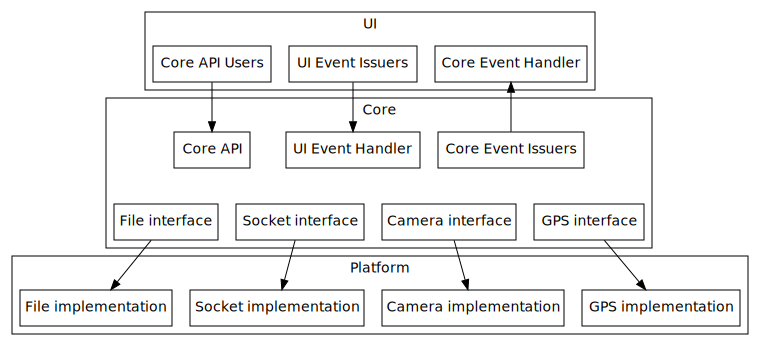
\includegraphics[scale=0.4]{08_2015_fig1}
\end{figure}

Приложение состоит из 3 частей:

\begin{itemize}
  \item UI "--- реализация UI, платформо"=зависимый код.
  \item Core "--- ядро/движок, платформо"=независимый код.
  \item Platform "--- реализация поддержки файловой системы, сети и устройств, платформо"=зависимый код.
\end{itemize}

Стрелки на схеме означают:

\begin{itemize}
  \item CoreAPIUsers $\rightarrow{}$ CoreAPI "--- Команды от UI к Core, например <<Перейти на такой"=то URL в таком"=то табе>>.
  \item UIEventIssuers $\rightarrow{}$ UIEventHandler "--- События в UI, которые должны быть обработаны Core, например клик мыши.
  \item CoreEventIssuers $\rightarrow{}$ CoreEventHandler "--- События в Core, которые должны быть обработаны в UI, например перерисовка области экрана.
  \item Some interface $\rightarrow{}$ Some implementation "--- вызовы кода, реализующие <<платформенный интерфейс>>, то есть отвечающего за поддержку файловой системы, сети и устройств на данной платформе.
\end{itemize}

Таким образом, для того, чтобы добавить поддержку какой"=либо платформы, надо:

\begin{itemize}
  \item Решить, какие возможности браузера и устройства хочется поддерживать на этой платформе.
  \item Разработать реализацию UI и платформенных интерфейсов, с учётом выбранных возможностей.
\end{itemize}

То есть, если какая"=то возможность браузера (например, поддержка GPS) не будет активирована на данной платформе "--- не надо и реализовывать платформенный интерфейс GPS"=устройства. Подробнее включение/отключение возможностей программы будет описано ниже.

\subsection*{Как решать проблемы}


\begin{figure}[h!]
  \centering
  \begin{tabular}{ p{4.3cm} p{6.2cm} } \hline
    \textbf{Проблема}                                          & \textbf{Решение}                                                                                      \\ \hline
    Разные скорости CPU и объёмы памяти                 & Включение/отключение возможностей на стадии компиляции                                         \\
    Разные размеры экранов и их количество              & Задание размера экрана/окна при инициализации/изменении                                        \\
    Разные устройства управления                        & Поддержка в UI layer, возможно частично в Platform layer                                       \\
    Разные дополнительные устройства (камера, GPS) & Поддержка в Platform layer, обязательный \verb@#ifdef SOME_DEVICE_SUPPORT@                          \\
    Разные компиляторы, в том числе и капризные (ADS)   & Ответственное использование С++ (namespaces, templates, exceptions, RTTI, global vars, static) \\
    Особые методы запуска приложений (BREW, P2K)        & Реализация UI как библиотеки                                                                   \\
    Разные API у разных операционных систем             & Поддержка в Platform layer                                                                     \\ \hline
  \end{tabular}
\end{figure}

Выше были упомянуты некоторые проблемы, присущие кроссплатформенной разработке. Приведенная таблица кратко описывает, как их решать.

\subsection*{Включение/отключение возможностей на стадии компиляции}

Некоторые платформы, например feature phones имеют не очень"=то много памяти, как для хранения кода приложения, так и для его работы. Отключение некоторого функционала приложения на стадии компиляции помогает уменьшить размер кода этого приложения, расход памяти, а также ускоряет его работу.

Также, чем менее мощны устройства определённой платформы "--- тем, как правило, меньший спектр встроенных устройств (камера, GPS, etc) они поддерживают. Код для неподдерживаемых встроенных устройств на данной платформе также следует исключать из компиляции.

Для того, чтобы реализовать отключаемую поддержку определённого функционала или устройств на стадии компиляции для определённой платформы, используется простой способ:

\begin{enumerate}
  \item Обрамить код поддержки отключаемого функционала или \linebreak устройства в \#ifdef SOME\_FEATURE\_SUPPORT.
  \item Описывать (\#define) или сбрасывать (\#undef) соответствующий макрос в глобальном заголовочном файле для соответствующей платформы.
\end{enumerate}

Ниже приведён фрагмент кода на C++, который иллюстрирует описанный способ:

\begin{verbatim}
    #define FEATURE_1_SUPPORT
    #undef  FEATURE_2_SUPPORT
        ...
        // Код feature 1 будет скомпилирован,
        // потому что решено поддерживать
        // feature 1 на этой платформе.
    #ifdef FEATURE_1_SUPPORT
        m_component_loader->LoadFeature1Data();
    #endif
        ...
        // Код feature 2 не будет скомпилирован,
        // потому что решено не поддерживать
        // feature 2 на этой платформе.
        // Это уменьшит размер исполняемого кода,
        // потребление памяти во время исполнения
        // и увеличит его скорость.
    #ifdef FEATURE_2_SUPPORT
        m_component_loader->LoadFeature2Data();
    #endif
        ...\end{verbatim}
\subsection*{Как ещё уменьшить размер кода}

Существуют также и другие способы уменьшить размер кода:

\begin{itemize}
  \item Использовать код повторно, удалять более неиспользуемый код
  \item Уменьшить размер временных буферов и/или их время жизни (совет для runtime)
  \item Больше использовать библиотеки платформы, не дублировать их функционал в коде приложения
  \item Урезать используемые third"=party библиотеки, всё"=таки включённые в приложение; таким же образом (\#undef FEATURE), как урезается основной код
  \item Избегать зависимостей от слабых мест компилятора, (пример: раздувание template"=кода)
  \item Кросс"=компилировать лучшим компилятором
  \item Компилировать в более компактный набор инструкций процессора (пример: Thumb для ARM)
  \item Сжимать код, в ROM или RAM
  \item Использовать плагины/оверлеи
  \item Исполнять части кода в другом месте (пример: Opera Mini)
\end{itemize}

\subsection*{Пример платформенного интерфейса}

Ниже приведён пример платформенного интерфейса для сокетa TCP. Реализовав этот платформенный интерфейс, разработчик \linebreak обеспечит работу TCP"=соединений на данной платформе. Для Unix"=подобной платформы реализация может использовать BSD sockets, для Windows "--- WinSock, для Telium OS "--- LinkLayer и т.~д.

\begin{verbatim}
    // Будет реализовано в платформенном коде.
    class TCPSocket
    {
        static TCPSocket* New();
        Status SetListener(TCPSocketListener* listener) = 0;

        Status Connect(const char* host, unsigned short 
port) = 0;
        Status Disconnect() = 0;
        Status Send(const char* data, size_t length, size_t& 
accepted_length) = 0;
        Status Recv(char* data, size_t length, size_t& 
received_length) = 0;
    };

    // Будет реализовано в коде ядра.
    class TCPSocketListener
    {
        Status OnConnected() = 0;
        Status OnDisconnected() = 0;
        Status OnDataSent(size_t length) = 0;
        Status OnDataAvailable(size_t length) = 0;
        Status OnError(Error code) = 0;
    };
\end{verbatim}
\end{document}

\documentclass[10pt, a5paper]{article}
\usepackage{pdfpages}
\usepackage{parallel}
\usepackage[T2A]{fontenc}
\usepackage{ucs}
\usepackage[utf8x]{inputenc}
\usepackage[polish,english,russian]{babel}
\usepackage{hyperref}
\usepackage{rotating}
\usepackage[inner=2cm,top=1.8cm,outer=2cm,bottom=2.3cm,nohead]{geometry}
\usepackage{listings}
\usepackage{graphicx}
\usepackage{wrapfig}
\usepackage{longtable}
\usepackage{indentfirst}
\usepackage{array}
\newcolumntype{P}[1]{>{\raggedright\arraybackslash}p{#1}}
\frenchspacing
\usepackage{fixltx2e} %text sub- and superscripts
\usepackage{icomma} % коскі ў матэматычным рэжыме
\PreloadUnicodePage{4}

\newcommand{\longpage}{\enlargethispage{\baselineskip}}
\newcommand{\shortpage}{\enlargethispage{-\baselineskip}}

\def\switchlang#1{\expandafter\csname switchlang#1\endcsname}
\def\switchlangbe{
\let\saverefname=\refname%
\def\refname{Літаратура}%
\def\figurename{Іл.}%
}
\def\switchlangen{
\let\saverefname=\refname%
\def\refname{References}%
\def\figurename{Fig.}%
}
\def\switchlangru{
\let\saverefname=\refname%
\let\savefigurename=\figurename%
\def\refname{Литература}%
\def\figurename{Рис.}%
}

\hyphenation{admi-ni-stra-tive}
\hyphenation{ex-pe-ri-ence}
\hyphenation{fle-xi-bi-li-ty}
\hyphenation{Py-thon}
\hyphenation{ma-the-ma-ti-cal}
\hyphenation{re-ported}
\hyphenation{imp-le-menta-tions}
\hyphenation{pro-vides}
\hyphenation{en-gi-neering}
\hyphenation{com-pa-ti-bi-li-ty}
\hyphenation{im-pos-sible}
\hyphenation{desk-top}
\hyphenation{elec-tro-nic}
\hyphenation{com-pa-ny}
\hyphenation{de-ve-lop-ment}
\hyphenation{de-ve-loping}
\hyphenation{de-ve-lop}
\hyphenation{da-ta-ba-se}
\hyphenation{plat-forms}
\hyphenation{or-ga-ni-za-tion}
\hyphenation{pro-gramming}
\hyphenation{in-stru-ments}
\hyphenation{Li-nux}
\hyphenation{sour-ce}
\hyphenation{en-vi-ron-ment}
\hyphenation{Te-le-pathy}
\hyphenation{Li-nux-ov-ka}
\hyphenation{Open-BSD}
\hyphenation{Free-BSD}
\hyphenation{men-ti-on-ed}
\hyphenation{app-li-ca-tion}

\def\progref!#1!{\texttt{#1}}
\renewcommand{\arraystretch}{2} %Іначай формулы ў матрыцы зліпаюцца з лініямі
\usepackage{array}

\def\interview #1 (#2), #3, #4, #5\par{

\section[#1, #3, #4]{#1 -- #3, #4}
\def\qname{LVEE}
\def\aname{#1}
\def\q ##1\par{{\noindent \bf \qname: ##1 }\par}
\def\a{{\noindent \bf \aname: } \def\qname{L}\def\aname{#2}}
}

\def\interview* #1 (#2), #3, #4, #5\par{

\section*{#1\\{\small\rm #3, #4. #5}}

\def\qname{LVEE}
\def\aname{#1}
\def\q ##1\par{{\noindent \bf \qname: ##1 }\par}
\def\a{{\noindent \bf \aname: } \def\qname{L}\def\aname{#2}}
}

\begin{document}
\title{Опыт выбора и применения современных систем мониторинга}
\author{Наим Шафиев, Баку, Азербайджан\footnote{\url{shafiev@gmail.com}, \url{http://lvee.org/ru/abstracts/159}}}
\maketitle
\begin{abstract}
Modern heterogeneous infrastructure, which contains different types of network devices and servers, needs modern monitoring systems. Also the main problem of finding proper solution is that it should  fulfil requirements of flexibility, openness, good support from community. 
The article presents an overview and experience  of modern free monitoring systems, which fulfil spoken above requirements in case of a middle"=size ISP.
\end{abstract}
\subsection*{Основные требования}

Проблема роста и взаимозаменяемости сотрудников для решения задач мониторинга и DevOps проявляются в любой компании при росте от нескольких человек до так называемого среднего размера.

Рассмотрим, какие основные требования предъявляются к системам мониторинга в современных условиях:

\begin{itemize}
  \item опрос агентами ресурсов (CPU, Disk I/O, Ram, Network) серверов;
  \item опрос сетевых устройств различных устройств (очень желательно,чтобы были готовые MIB);
  \item опрос VMware"=серверов;
  \item гибкая система оповещений с многоуровневой системой зависимости;
  \item opensource.
\end{itemize}

Также очень важны понятная документация и легкий старт "--- как минимум, для взаимозаменяемости сотрудников.

\subsection*{Практика использования}

Ниже представлены особенности, родившиеся из опыта поиска и использования различных решений (таких, как Nagios, Zabbix, LibreNMS, NetXMS) на  размере более 500 активных узлов в ISP среднего размера.
Рассмотрев все эти решения мы пришли к следующим выводам:

\begin{itemize}
  \item Nagios "--- к сожалению, началось разделение на бесплатную Core"=версию и XI"=версию, все это привело к появлению более технологичного форка Icinga. Также из минусов стоит отметить не доведенную до промышленного использования многоуровневую систему взаимосвязи объектов и сервисов.
  \item Zabbix "--- лучший opensource"=продукт, возможен высокий уровень детализации данных, развитое community. Из минусов "--- сложность в настройке, сложно дорабатывать.
  \item LibreNMS "--- наиболее перспективный свободный продукт. \linebreak Очень легкий старт (сравнимый с PRTG), использование стандартных компонентов. Включает огромное количество готовых MIB. Из минусов "--- невозможность без осложнений задать детализированные графики (менее 5 минут), нету развитой системы зависимостей (в данный момент автор решает эту задачу).
  \item NetXMS "--- один из наиболее технологичных продуктов индустрии. Содержит высокопроизводительное ядро, возможен высокий уровень детализации и другие стандартные для проприетарных систем функции. Из минусов отмечается сложный старт, ручная настройка, малое community.
\end{itemize}

Автор в данный момент дорабатывает LibreNMS для замены связки Nagios/Zabbix+MRTG.

\end{document}

\documentclass[10pt, a5paper]{article}
\usepackage{pdfpages}
\usepackage{parallel}
\usepackage[T2A]{fontenc}
\usepackage{ucs}
\usepackage[utf8x]{inputenc}
\usepackage[polish,english,russian]{babel}
\usepackage{hyperref}
\usepackage{rotating}
\usepackage[inner=2cm,top=1.8cm,outer=2cm,bottom=2.3cm,nohead]{geometry}
\usepackage{listings}
\usepackage{graphicx}
\usepackage{wrapfig}
\usepackage{longtable}
\usepackage{indentfirst}
\usepackage{array}
\newcolumntype{P}[1]{>{\raggedright\arraybackslash}p{#1}}
\frenchspacing
\usepackage{fixltx2e} %text sub- and superscripts
\usepackage{icomma} % коскі ў матэматычным рэжыме
\PreloadUnicodePage{4}

\newcommand{\longpage}{\enlargethispage{\baselineskip}}
\newcommand{\shortpage}{\enlargethispage{-\baselineskip}}

\def\switchlang#1{\expandafter\csname switchlang#1\endcsname}
\def\switchlangbe{
\let\saverefname=\refname%
\def\refname{Літаратура}%
\def\figurename{Іл.}%
}
\def\switchlangen{
\let\saverefname=\refname%
\def\refname{References}%
\def\figurename{Fig.}%
}
\def\switchlangru{
\let\saverefname=\refname%
\let\savefigurename=\figurename%
\def\refname{Литература}%
\def\figurename{Рис.}%
}

\hyphenation{admi-ni-stra-tive}
\hyphenation{ex-pe-ri-ence}
\hyphenation{fle-xi-bi-li-ty}
\hyphenation{Py-thon}
\hyphenation{ma-the-ma-ti-cal}
\hyphenation{re-ported}
\hyphenation{imp-le-menta-tions}
\hyphenation{pro-vides}
\hyphenation{en-gi-neering}
\hyphenation{com-pa-ti-bi-li-ty}
\hyphenation{im-pos-sible}
\hyphenation{desk-top}
\hyphenation{elec-tro-nic}
\hyphenation{com-pa-ny}
\hyphenation{de-ve-lop-ment}
\hyphenation{de-ve-loping}
\hyphenation{de-ve-lop}
\hyphenation{da-ta-ba-se}
\hyphenation{plat-forms}
\hyphenation{or-ga-ni-za-tion}
\hyphenation{pro-gramming}
\hyphenation{in-stru-ments}
\hyphenation{Li-nux}
\hyphenation{sour-ce}
\hyphenation{en-vi-ron-ment}
\hyphenation{Te-le-pathy}
\hyphenation{Li-nux-ov-ka}
\hyphenation{Open-BSD}
\hyphenation{Free-BSD}
\hyphenation{men-ti-on-ed}
\hyphenation{app-li-ca-tion}

\def\progref!#1!{\texttt{#1}}
\renewcommand{\arraystretch}{2} %Іначай формулы ў матрыцы зліпаюцца з лініямі
\usepackage{array}

\def\interview #1 (#2), #3, #4, #5\par{

\section[#1, #3, #4]{#1 -- #3, #4}
\def\qname{LVEE}
\def\aname{#1}
\def\q ##1\par{{\noindent \bf \qname: ##1 }\par}
\def\a{{\noindent \bf \aname: } \def\qname{L}\def\aname{#2}}
}

\def\interview* #1 (#2), #3, #4, #5\par{

\section*{#1\\{\small\rm #3, #4. #5}}

\def\qname{LVEE}
\def\aname{#1}
\def\q ##1\par{{\noindent \bf \qname: ##1 }\par}
\def\a{{\noindent \bf \aname: } \def\qname{L}\def\aname{#2}}
}

\begin{document}
\title{Coreboot. Практическое знакомство со свободной альтернативой BIOS}
\author{Николай Стомчик, Минск, Беларусь\footnote{\url{mn3m00@gmail.com}, \url{http://lvee.org/en/abstracts/160}}}
\maketitle
\begin{abstract}
In modern Open Source world we need an open alternative to the proprietary product called BIOS. This alternative exists and is called coreboot. Coreboot is not fully equal to BIOS, it's only does initialization of RAM, execution of binary vendor blobs and starting some payload. The report main task is to cover how to start using it.
\end{abstract}
\subsection*{Введение}

Для построения полностью свободного стека ПО необходимо иметь свободную альтернативу проприетарным прошивкам \linebreak(firmware): классическому BIOS, либо UEFI в более новых системах. Такая альтернатива есть, и она называется coreboot.

Практические причины для использования CoreBoot \cite{bib1} могут быть:

\begin{itemize}
  \item Нужда в свободной альтернативе UEFI;
  \item Создание единого командно"=интерфейсного слоя в уровне \linebreak <<прошивки>> для кластерных решений на различных системах и архитектурах;
  \item Ускорить загрузку системы до ОС (до $\sim$~3~с)
  \item Разместить всю ОС (GNU/Linux, FreeBSD или другую) во flash"=памяти, позволив работать в режиме восстановления либо в полноценном режиме без использования жесткого диска;
  \item Общеобразовательные :)
  \item Предотвращение угрозы полумифического BadBIOS \cite{bib2, bib3};
\end{itemize}

\subsection*{Процесс загрузки Coreboot}

В процессе загрузки, устройство с coreboot проходит через следующие стадии:

\begin{figure}[h!]
  \centering
  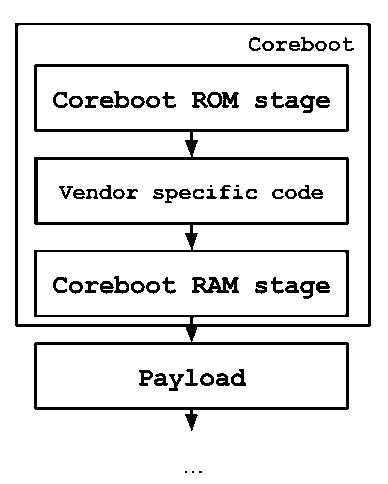
\includegraphics[scale=0.4]{10_2015_fig1}
\end{figure}

\begin{itemize}
  \item ROM stage "--- инициализация памяти и начальная инициализация чипсета; помимо общей схемы действий эта часть по понятным причинам очень специфична для конкретного оборудования, и здесь в обязательном порядке присутствует выполнение некоторых частей бинарной прошивки, которая определена производителем как обязательная для инициализации RAM, CPU или других системных устройств;
  \item RAM stage "--- нумерация устройств, назначение ресурсов, создание таблицы ACPI, SMM handler;
  \item Payload "--- выполнение некой полезной нагрузки, которая в \linebreak свою очередь может быть неким приложением либо загрузить операционную систему.
\end{itemize}

Coreboot не является полной заменой BIOS, т.к. не содержит никакой активной части по выполнению <<полезных действий>>: эта часть вынесена в отдельный модуль, называемый <<payload>> (полезная нагрузка). Достоинство такого разделения "--- возможность менять payload. Например, автором в качестве payload использован SeaBIOS, но есть альтернативы, такие как <<GRUB2>>, <<OpenBIOS>>. Можно <<выполнить>> в качестве payload ядро Linux или FreeBSD, а можно создать собственный: например, очень нужный в реальной практике payload, который пишет <<hello world>> и завершается:
\begin{verbatim}
 include <libpayload.h>
 int main(void)
 {
     printf("Hello, world from CoreBoot! :)\n");
     return 0;
 }
\end{verbatim}
Сборка этого шедевра функциональности может быть выполнена следующим способом:

\verb! $ lpgcc -o hello.elf hello.c!

После чего, данный Payload необходимо добавить в Ваш бинарный файл Coreboot.rom и можно перейти на этап загрузки его в ПЗУ.

\subsection*{Подготовка coreboot к прошивке}

По понятным причинам поддержка всего многообразия чипсетов и материнских плат проектом coreboot оставляет желать лучшего. Однако, если ваше оборудование попало в число поддерживаемых, процедура перепрограммирования может оказаться не самая простая, особенно в случае если производитель ноутбука либо компьютера поспешил обезопасить себя от желающих самостоятельно заменить базовую микро"=программу.

В частности, подготовительные шаги для установки coreboot на основе личного опыта автора по перепрошивке ThinkPad x201\cite {bib4} выглядели следующим образом:

\begin{itemize}
  \item тщательное изучение документации по разборке ноутбука, чтобы отыскать чипы памяти BIOS и CMOS;
  \item чтение datasheet'ов на ROM и выяснение специфики его программирования;
  \item покупка (либо сборка) программатора и разъёмов (SOIC"=8P) для ISP программирования;
  \item извлечение videorom.bin из оригинального проприетарного \linebreak BIOS, которую можно получить из ОЗУ в процессе работы системы;
  \item создание резервной копии firmware с помощью программного или аппаратного программатора (эксперименты с подобными материями быстро излечивают от неоправданного оптимизма);
  \item клонирование coreboot и его зависимостей из git, выполнение `make menuconfig' и `make', с последующими \emph{n} часами сборки с удовлетворением всех зависимостей;
  \item программирование в ПЗУ результирующего бинарного файла;
  \item многочасовое тестирование компьютера с новой прошивкой, с использованием нагрузочных тестов и проверкой всего оборудования.
\end{itemize}

\begin{figure}[h!]
  \centering
  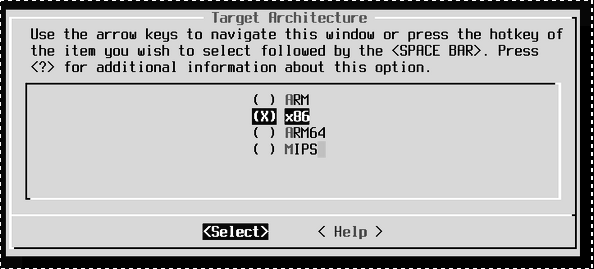
\includegraphics[scale=0.4]{10_2015_fig2}
\end{figure}

Саму запись микропрограммы в постоянную память можно выполнить из Linux её штатными средствами "--- <<flashrom>>, либо, если этот этап завершился неудачей "--- аппаратным программатором.  В случае с Thinkpad x201 для программирования MX25L6445E (8MB Serial Flash) подходят программаторы:

\begin{itemize}
  \item BusPirate v4;
  \item minipro TL866C;
  \item Raspberry PI;
  \item любой другой, который умеет программировать через SPI.
\end{itemize}

Из"=за того, что программная перепрошивка оказалась заблокирована вендором (а способ разблокировки, применяемый для обновления фирменной прошивки, на данный момент неизвестен), для LENOVO Thinkpad x201 пришлось воспользоваться аппаратным программатором minipro TL866. При работе из GNU/Linux команда перепрошивки должна выглядеть примерно следующим образом:

\begin{verbatim}./minipro -i -p "MX25L6445E @SOP8" -w {Patch_for_your_
coreboot}build/coreboot.rom\end{verbatim}

\begin{figure}[h!]
  \centering
  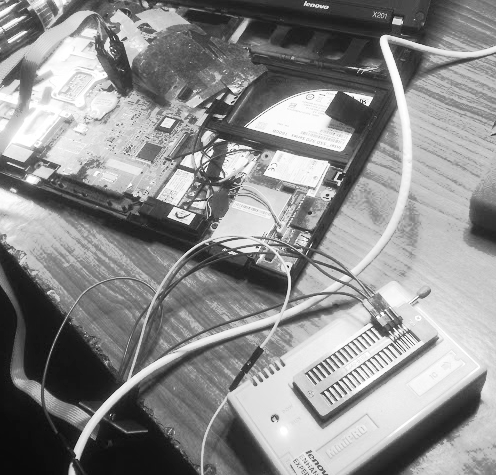
\includegraphics[scale=0.4]{10_2015_fig3}
\end{figure}

\subsection*{Советы по внутрисхемному программированию}

\begin{itemize}
  \item Важно следить за уровнем питания микросхемы на плате. Если питания не достаточно, есть смысл воспользоваться внешним блоком питания. Обычный стандартный блок ATX для таких задач вполне подходит (необходимо +3.3V);
  \item Для получения корректных результатов считывания и записи <<Земля>> (GND) программатора, корпуса ноутбука и блока питания должны быть соединены;
  \item Перед записью будет не лишним попробовать прочитать содержимое микросхемы N раз и проверить контрольные суммы "--- SHA или MD5. Если они не совпадают, проблема наверняка кроется в двух предыдущих пунктах.
\end{itemize}

\subsection*{Работоспособность после прошивки}

В результате экспериментов с ThinkPad x201 были выявлены следующие мелкие баги (которые, возможно, на момент чтения этой статьи уже будут исправлены):

\begin{itemize}
  \item ограничение <<на перегрев CPU>> теперь отсутствует, что требует добавить ещё один скрипт проверки на перегрев, либо понизить немного частоту CPU до стабильной, что бы этот перегрев и не возникал;
  \item каждые 10 минут возникает <<засыпание>> экрана, вне зависимости от установок xset (Исправляется \verb!xset -dpms off!);
  \item при подключенном втором дисплее перестает регулироваться яркость подсветки основного дисплея используя горячие клавиши;
  \item понадобилось переписать скрипт регулировавший частоту процессора из"=за новых значений шага для частоты CPU;
  \item проигрывание звука на колонках отключается программно, то есть при включенных наушниках можно включить воспроизведение на встроенных динамиках ноутбука;
\end{itemize}

Однако список работающего функционала оказался внушительным:

\begin{itemize}
  \item 3G GPRS modem;
  \item 4G+4G RAM;
  \item функциональные клавиши ThinkPad (фонарик, громкость);
  \item расширения VT"=x процессора;
  \item аппаратная поддержка AES в CPU;
  \item WIFI;
  \item Ethernet;
  \item Все порты ноутбука (USB, DP, HDMI, DSUB), а также док"=станция;
  \item Устройство считывания отпечатков пальцев;
  \item Управление питанием устройства, контроль за состоянием батареи.
\end{itemize}

Время загрузки микропрограммы, инициализации всего аппаратного обеспечения и передача управления начальному загрузчику ОС (GRUB2) сократилось с $\sim$ 50 с до $\sim$ 4 с, и при том большую часть из этого времени SeaBIOS ожидает нажатия F12 для выбора устройства загрузки. Хотя ускорение загрузки не являлось целью данной работы, нельзя не отметить, что логотип coreboot соответствует его значению:

\begin{figure}[h!]
  \centering
  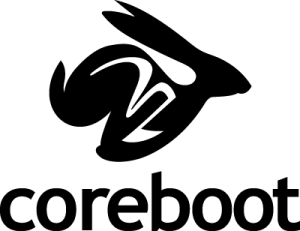
\includegraphics[scale=0.3]{10_2015_fig4}
\end{figure}

Конечно, данное обстоятельно не может не радовать.

\subsection*{Отладка}

Подготовленный payload можно протестировать в эмуляторе \linebreak QEMU"=KVM перед запуском, чтобы удостовериться, что всё работает как требуется. В самом же устройстве можно использовать традиционный для этих задач индикатор POST"=кодов, отображающий значения, отправленные в порт 80h, последовательный порт "--- либо PC"=speaker как средства диагностики состояния и процесса загрузки.

\begin{figure}[h!]
  \centering
  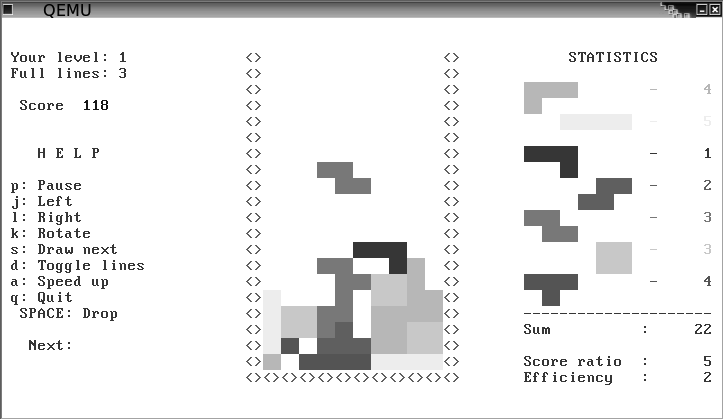
\includegraphics[scale=0.55]{10_2015_fig5}
\end{figure}


\begin{thebibliography}{9}
\bibitem{bib1} {\href{http://www.coreboot.org/}{http://www.coreboot.org}}
\bibitem{bib2} {Bruce Schneier. badBIOS // Schneier on Security. \href{https://www.schneier.com/blog/archives/2013/11/badbios.html}{https://www.schneier.com/blog/archives/2013/11/badbios.html}}
\bibitem{bib3} {Jonathan Brossard. Hardware backdooring is practica. // DEFCON 20 presentation. \href{http://www.slideshare.net/endrazine/defcon-hardware-backdooring-is-practical}{http://www.slideshare.net/endrazine/defcon-hardware-backdooring-is-practical}}
\bibitem{bib4} {\href{https://github.com/mn3m0nic/ffts/blob/master/thinkpad.md}{github.com/mn3m0nic/ffts/blob/master/thinkpad.md}}\end{thebibliography}
\end{document}

\documentclass[10pt, a5paper]{article}
\usepackage{pdfpages}
\usepackage{parallel}
\usepackage[T2A]{fontenc}
\usepackage{ucs}
\usepackage[utf8x]{inputenc}
\usepackage[polish,english,russian]{babel}
\usepackage{hyperref}
\usepackage{rotating}
\usepackage[inner=2cm,top=1.8cm,outer=2cm,bottom=2.3cm,nohead]{geometry}
\usepackage{listings}
\usepackage{graphicx}
\usepackage{wrapfig}
\usepackage{longtable}
\usepackage{indentfirst}
\usepackage{array}
\newcolumntype{P}[1]{>{\raggedright\arraybackslash}p{#1}}
\frenchspacing
\usepackage{fixltx2e} %text sub- and superscripts
\usepackage{icomma} % коскі ў матэматычным рэжыме
\PreloadUnicodePage{4}

\newcommand{\longpage}{\enlargethispage{\baselineskip}}
\newcommand{\shortpage}{\enlargethispage{-\baselineskip}}

\def\switchlang#1{\expandafter\csname switchlang#1\endcsname}
\def\switchlangbe{
\let\saverefname=\refname%
\def\refname{Літаратура}%
\def\figurename{Іл.}%
}
\def\switchlangen{
\let\saverefname=\refname%
\def\refname{References}%
\def\figurename{Fig.}%
}
\def\switchlangru{
\let\saverefname=\refname%
\let\savefigurename=\figurename%
\def\refname{Литература}%
\def\figurename{Рис.}%
}

\hyphenation{admi-ni-stra-tive}
\hyphenation{ex-pe-ri-ence}
\hyphenation{fle-xi-bi-li-ty}
\hyphenation{Py-thon}
\hyphenation{ma-the-ma-ti-cal}
\hyphenation{re-ported}
\hyphenation{imp-le-menta-tions}
\hyphenation{pro-vides}
\hyphenation{en-gi-neering}
\hyphenation{com-pa-ti-bi-li-ty}
\hyphenation{im-pos-sible}
\hyphenation{desk-top}
\hyphenation{elec-tro-nic}
\hyphenation{com-pa-ny}
\hyphenation{de-ve-lop-ment}
\hyphenation{de-ve-loping}
\hyphenation{de-ve-lop}
\hyphenation{da-ta-ba-se}
\hyphenation{plat-forms}
\hyphenation{or-ga-ni-za-tion}
\hyphenation{pro-gramming}
\hyphenation{in-stru-ments}
\hyphenation{Li-nux}
\hyphenation{sour-ce}
\hyphenation{en-vi-ron-ment}
\hyphenation{Te-le-pathy}
\hyphenation{Li-nux-ov-ka}
\hyphenation{Open-BSD}
\hyphenation{Free-BSD}
\hyphenation{men-ti-on-ed}
\hyphenation{app-li-ca-tion}

\def\progref!#1!{\texttt{#1}}
\renewcommand{\arraystretch}{2} %Іначай формулы ў матрыцы зліпаюцца з лініямі
\usepackage{array}

\def\interview #1 (#2), #3, #4, #5\par{

\section[#1, #3, #4]{#1 -- #3, #4}
\def\qname{LVEE}
\def\aname{#1}
\def\q ##1\par{{\noindent \bf \qname: ##1 }\par}
\def\a{{\noindent \bf \aname: } \def\qname{L}\def\aname{#2}}
}

\def\interview* #1 (#2), #3, #4, #5\par{

\section*{#1\\{\small\rm #3, #4. #5}}

\def\qname{LVEE}
\def\aname{#1}
\def\q ##1\par{{\noindent \bf \qname: ##1 }\par}
\def\a{{\noindent \bf \aname: } \def\qname{L}\def\aname{#2}}
}

\begin{document}
\title{Qucs "--- свободный симулятор электронных схем: новые возможности релиза 0.0.19}
\author{Вадим Кузнецов, Калуга, РФ\footnote{\url{ra3xdh@gmail.com}, \url{http://lvee.org/en/abstracts/162}}}
\maketitle
\begin{abstract}
Qucs (Quite Universal Circuit Simulator) is open source cir\-cuit simulation CAD tool. The main features of Qucs are conside\-red. New features of upcoming 0.0.19 release and spice4qucs subsystem are reviewed. Spice4qucs allows to simulate circuits from Qucs using external simulator kernels such as Ngspice and Xyce.
\end{abstract}
В настоящее время существует не так уж и много open"=source САПР. Тем не менее, среди САПР для электроники (EDA) есть весьма достойные продукты. Доклад посвящён симулятору электронных схем с открытым исходным кодом Qucs \url{http://qucs.sourceforge.net}. Qucs написан на С++ с использованием фреймворка Qt4. Qucs является кроссплатформенным и выпущен для ОС Linux, Windows и MacOS. Текущей версией проекта является 0.0.18. В настоящее время ведётся подготовка к релизу версии 0.0.19.

Разработку данной САПР начали в 2004 году немцы Michael Margraf и Stefan Jahn (в настоящее время не активны). Сейчас Qucs разрабатывается интернациональной командой, в которую входит автор статьи. Руководителями проекта являются Frans Schreuder и Guilherme Torri.

Qucs позволяет проводить следующие виды моделирования:

\begin{enumerate}
\item Моделирование на постоянном токе (DC analysis)
\item Моделирование в частотной области (AC analysis)
\item Моделирование во временной области (Transient analysis)
\item Параметрический анализ (Parameter sweep)
\item Моделирование S"=параметров в частотной области (S"=parame\-ter)
\item Синтез пассивных фильтров, согласованных схем, расчёт коаксиальных 
и микрополосковых линий.
\end{enumerate}

Результаты моделирования можно визуализировать в виде графиков в декартовых (2D и 3D) и полярных координатах, а также в виде таблиц и диаграмм Смита.

В настоящее время существуют следующие open"=source средства моделирования 
электронных схем:
\begin{enumerate}
\item Ngspice \url{http://ngspice.org} "--- консольный симулятор элект\-ронных схем. 
Совместим с индустриальным стандартом моделей электронных компонентов SPICE.
\item Xyce \url{http://xyce.sandia.gov} "--- новейший spice"=совместимый консольный 
симулятор, поддерживает параллельные вычисления через openMPI. Вышел в 2014 
году. Совместим с индустриальным стандартом моделей электронных компонентов 
SPICE.
\end{enumerate}

Недостатком вышеперечисленных симуляторов является отсутствие графического 
интерфейса, что сильно затрудняет ввод схемы. Для преодоления данного 
недостатка был разработан набор патчей spice4qucs, разработанный автором 
совместно с Mike Brinson (London Metropolitan University). Данный набор патчей позволяет использовать Qucs в качестве фронтенда для Ngspice или Xyce. Включение данного набора патчей в основную ветку ожидается в версии 0.0.19. В настоящее время поддерживаются все основные виды моделирования и компоненты. Текущий статус разработки можно отследить в репозитории проекта: \url{http://github.com/Qucs/qucs/issues/77}

Подсистема spice4qucs позволяет:
\begin{enumerate}
\item Моделировать схему Qucs при помощи внешнего симулятора Ngspice или Xyce
\item Использовать систему параметрического моделирования, совместимую со SPICE
\item Использовать постпроцессор Ngnutmeg
\item Использовать SPICE"=модели из документации электронных компонентов без 
ограничений
\item Использовать специфические виды моделирования, совместимые с Ngspice и 
Xyce: (Fourier analysis, Distortion analysis, Noise analysis)
\item Проводить моделирование при помощи скрипта Ngnutmeg, задаваемого 
пользователем.
\end{enumerate}

Функция поддержки внешних симуляторов, реализуемая подсистемой Spice4qucs, не 
имеет аналогов в проприетарном ПО.

Будущими задачами является разработка в следующих перспективных направлениях:
\begin{enumerate}
\item Расширение библиотеки компонентов
\item Разработка редактора библиотек
\item Разработка системы связи с KiCAD
\item Поддержка электромагнитного симулятора openEMS
\item Разработка системы экспорта моделей в формат Verilog"=A
\end{enumerate}

Таким образом, можно сделать вывод о том, что Qucs представляет собой 
быстроразвивающуюся САПР, по отдельным параметрам не уступающую проприетарным аналогам.  
можно рекомендовать Qucs для моделирования электронных схем в академических 
целях, на малых предприятиях и индивидуальным разработчикам электроники, а в 
некоторых случаях Qucs можно использовать и на крупных предприятиях для замены проприетарного ПО, закупаемого за рубежом.

\end{document}

\documentclass[10pt, a5paper]{article}
\usepackage{pdfpages}
\usepackage{parallel}
\usepackage[T2A]{fontenc}
\usepackage{ucs}
\usepackage[utf8x]{inputenc}
\usepackage[polish,english,russian]{babel}
\usepackage{hyperref}
\usepackage{rotating}
\usepackage[inner=2cm,top=1.8cm,outer=2cm,bottom=2.3cm,nohead]{geometry}
\usepackage{listings}
\usepackage{graphicx}
\usepackage{wrapfig}
\usepackage{longtable}
\usepackage{indentfirst}
\usepackage{array}
\newcolumntype{P}[1]{>{\raggedright\arraybackslash}p{#1}}
\frenchspacing
\usepackage{fixltx2e} %text sub- and superscripts
\usepackage{icomma} % коскі ў матэматычным рэжыме
\PreloadUnicodePage{4}

\newcommand{\longpage}{\enlargethispage{\baselineskip}}
\newcommand{\shortpage}{\enlargethispage{-\baselineskip}}

\def\switchlang#1{\expandafter\csname switchlang#1\endcsname}
\def\switchlangbe{
\let\saverefname=\refname%
\def\refname{Літаратура}%
\def\figurename{Іл.}%
}
\def\switchlangen{
\let\saverefname=\refname%
\def\refname{References}%
\def\figurename{Fig.}%
}
\def\switchlangru{
\let\saverefname=\refname%
\let\savefigurename=\figurename%
\def\refname{Литература}%
\def\figurename{Рис.}%
}

\hyphenation{admi-ni-stra-tive}
\hyphenation{ex-pe-ri-ence}
\hyphenation{fle-xi-bi-li-ty}
\hyphenation{Py-thon}
\hyphenation{ma-the-ma-ti-cal}
\hyphenation{re-ported}
\hyphenation{imp-le-menta-tions}
\hyphenation{pro-vides}
\hyphenation{en-gi-neering}
\hyphenation{com-pa-ti-bi-li-ty}
\hyphenation{im-pos-sible}
\hyphenation{desk-top}
\hyphenation{elec-tro-nic}
\hyphenation{com-pa-ny}
\hyphenation{de-ve-lop-ment}
\hyphenation{de-ve-loping}
\hyphenation{de-ve-lop}
\hyphenation{da-ta-ba-se}
\hyphenation{plat-forms}
\hyphenation{or-ga-ni-za-tion}
\hyphenation{pro-gramming}
\hyphenation{in-stru-ments}
\hyphenation{Li-nux}
\hyphenation{sour-ce}
\hyphenation{en-vi-ron-ment}
\hyphenation{Te-le-pathy}
\hyphenation{Li-nux-ov-ka}
\hyphenation{Open-BSD}
\hyphenation{Free-BSD}
\hyphenation{men-ti-on-ed}
\hyphenation{app-li-ca-tion}

\def\progref!#1!{\texttt{#1}}
\renewcommand{\arraystretch}{2} %Іначай формулы ў матрыцы зліпаюцца з лініямі
\usepackage{array}

\def\interview #1 (#2), #3, #4, #5\par{

\section[#1, #3, #4]{#1 -- #3, #4}
\def\qname{LVEE}
\def\aname{#1}
\def\q ##1\par{{\noindent \bf \qname: ##1 }\par}
\def\a{{\noindent \bf \aname: } \def\qname{L}\def\aname{#2}}
}

\def\interview* #1 (#2), #3, #4, #5\par{

\section*{#1\\{\small\rm #3, #4. #5}}

\def\qname{LVEE}
\def\aname{#1}
\def\q ##1\par{{\noindent \bf \qname: ##1 }\par}
\def\a{{\noindent \bf \aname: } \def\qname{L}\def\aname{#2}}
}

\begin{document}
\title{Создание робота для Roborace}
\author{Дмитрий Склипус, Брест, Беларусь\footnote{\url{sklipus@gmail.com}, \url{http://lvee.org/en/abstracts/163}}}
\maketitle
\begin{abstract}
Author shares his development experience of Arduino"=based robots targeted at Roborace competitions. Specifics of the com\-petition is explained as far as some details of the hardware platform and the contol algorythm.
\end{abstract}
\subsection*{Специфика Roborace}

Roborace "--- это состязания, в которых соревнуются роботы"=автомобили на специальной кольцевой трассе. Можно провести некоторую аналогию между Roborace и гонками Формулы 1, за исключением двух моментов.

\begin{itemize}
  \item Во"=первых, вместо полномасштабных гоночных болидов участвуют уменьшенные модели авто и оригинальные конструкции с габаритными и весовыми ограничениями (максимальные ШхД=25х50 см и вес до 3 кг).
  \item Во"=вторых, вместо пилотов автомобилем управляет бортовой компьютер, который анализирует показания различных датчиков и ориентирует автомобиль на трассе, выбирает скорость движения, предотвращает столкновения с препятствиями и соперниками. Собственно <<поведение>> авто на трассе определяется управляющей программой бортового компьютера.
\end{itemize}

Roborace проводится в виде чемпионата, состоящего из этапов, которые организуются в различных городах Беларуси и за рубежом. Участие в чемпионате принимают как конструкции начального уровня (например, на базе конструктора типа LEGO), так и сложные робототехнические устройства. Регламенты соревнований формируются таким образом, чтобы охватить как можно более широкий спектр характеристик и возможностей робототехнических конструкций.

\begin{figure}[h!]
  \centering 
  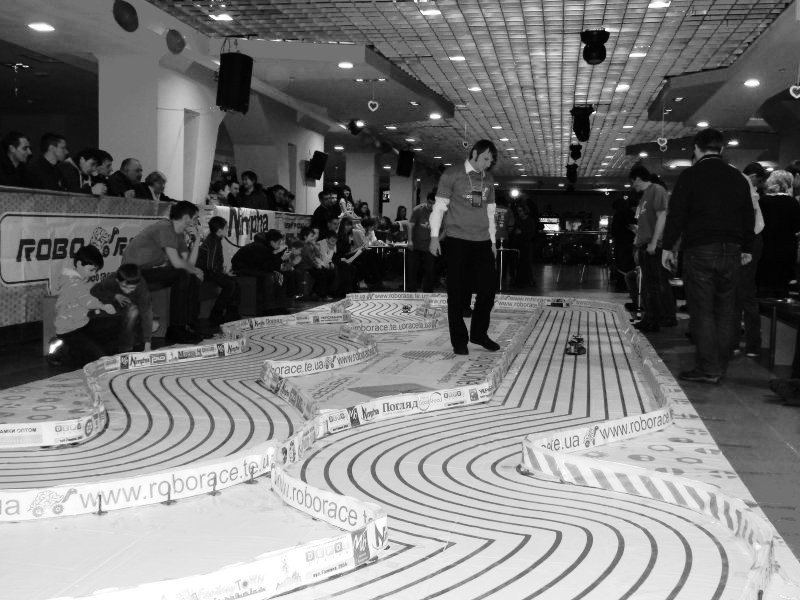
\includegraphics[scale=0.35]{12_2015_fig1}
  \caption{Трасса для гонок роботов}\label{sklipus1}
\end{figure}

Рассмотрим трассу, изображенную на рисунке \ref{sklipus1}, по которой предстоит перемещаться роботу. Обязательными элементами являются черные линии и стенки. Исходя из этого можно строить стратегию движения робота по трассе: например, оборудовать робота датчиками черной линии и использовать линии трассы для навигации, или установить дальномеры для обнаружения препятствий и двигаться вдоль стенок.

В рамках данной статьи представлен один из роботов, разработанный мной для Roborace по второй стратегия (движение на основе показаний дальномеров).

\subsection*{Этапы создания робота}

Создание робота для Roborace начинается с выбора шасси. Сейчас магазины предлагают большой выбор гусеничных и колесных платформ. Я рекомендую остановиться на классической схеме, когда задние колеса приводятся в движение электродвигателем, а передние управляются сервоприводом \cite{bib1}. На рисунке \ref{sklipus2} изображен робот для Roborace, построенный по подобной схеме.

\begin{figure}[h!]
  \centering 
  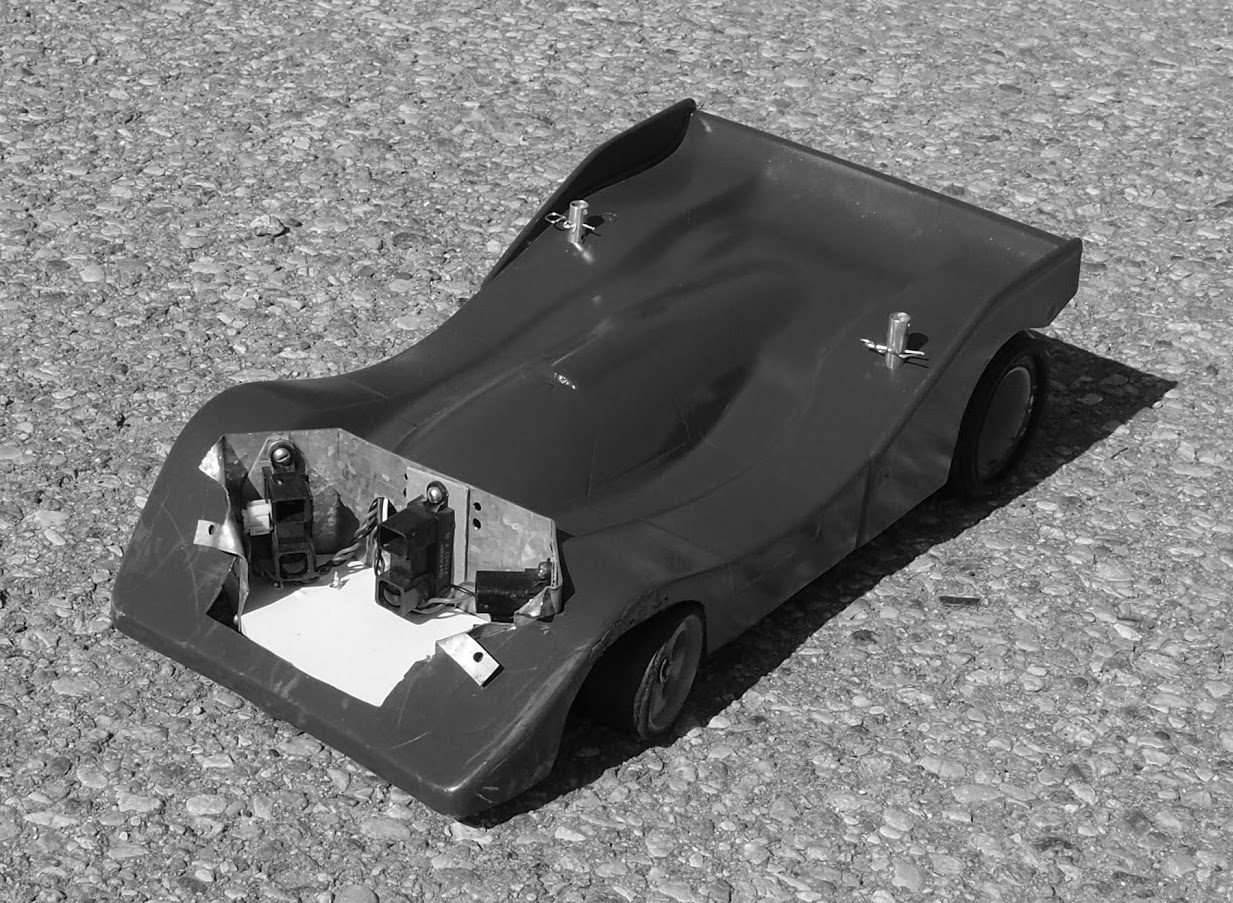
\includegraphics[scale=0.15]{12_2015_fig2}
  \caption{Робот}\label{sklipus2}
\end{figure}

Мне повезло за небольшие деньги приобрести модель в местном клубе радио"=моделистов (читатели могут попытаться сделать то же самое в своем регионе: обычно у них много устаревших моделей). Так как в приобретенной модели не было тягового электродвигателя, на нее был установлен установил купленный 12"=вольтный мотор. Можно было также использовать обычную игрушку: они обычно довольно живучи, и требуется только модифицировать рулевое управление.

Так как в моем случае сервопривод уже был установлен, с ним проблем не возникло.

Следующий этап "--- выбор платы управления. Тут есть множество вариантов. Я выбрал Arduino как самый простой вариант. То же можно порекомендовать и читателю, особенно при недостатке опыта. Исходя из моего достаточно большого опыта, для таких роботов достаточно обычных 8"=битных микроконтроллеров. Поэтому если не планируется использовать для отслеживания движений робота камеру, не стоит усложнять его более мощным процессором.

Сервопривод можно напрямую подключить к Arduino "--- например, через sensor shield, изображенный на рисунке \ref{sklipus3}. К нему также удобно подключать датчики.

\begin{figure}[h!]
  \centering 
  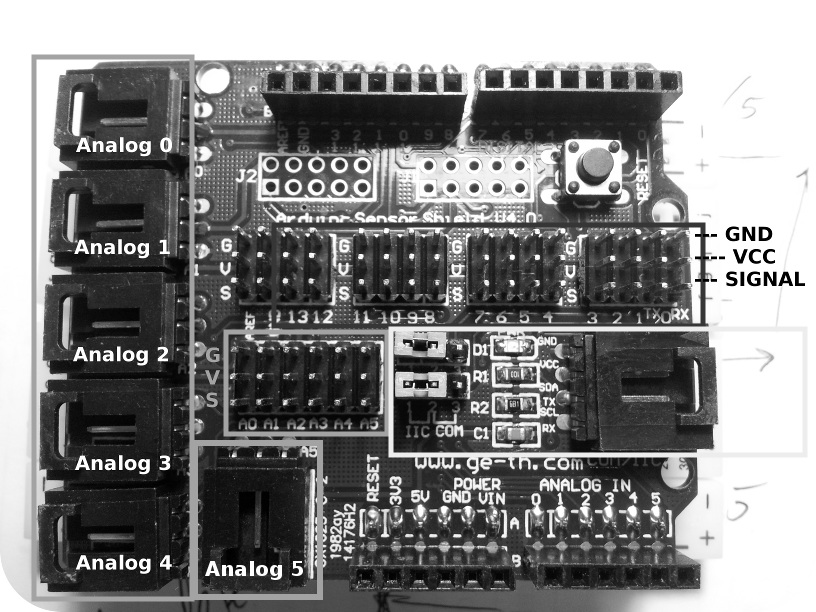
\includegraphics[scale=0.3]{12_2015_fig3}
  \caption{Sensor shield v4}\label{sklipus3}
\end{figure}

Мотор подключить к Arduino напрямую не получится. Нужно использовать специальные Motor Driver. Сейчас из достаточно много в продаже, и есть инструкции по подключению. Я использовал Motor Driver, разработанный в нашей лаборатории (рис. \ref{sklipus4}).

\begin{figure}[h!]
  \centering 
  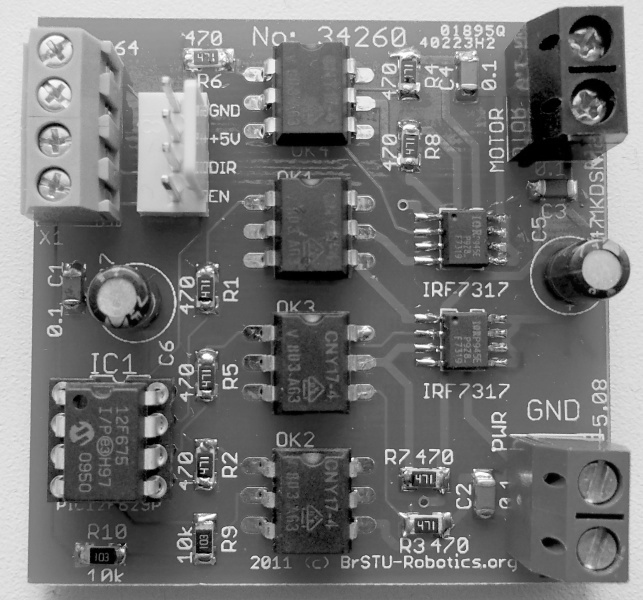
\includegraphics[scale=0.2]{12_2015_fig4}
  \caption{Motor driver}\label{sklipus4}
\end{figure}

В соревнованиях роботов приходится много внимания уделять батареям. Я использую литий"=полимерные аккумуляторы. Они \linebreak очень хорошо себя зарекомендовали. Один из хаков, которые я применяю в своем роботе, касается преобразователя напряжения. Штатный преобразователь в Arduino не очень хорош, поэтому для экономии энергии аккумулятора неплохо использовать Step"=Down регулятор \cite{bib2}. Конечно, можно использовать и обычный линейный преобразователь.

Самая главная часть робота это датчики "--- то, что обеспечивает его информацией об окружающем мире, о препятствиях и о других роботах. В средней ценовой категории мы можем выбирать из \emph{ультразвуковых} и \emph{инфракрасных} датчиков. В своем роботе я использую инфракрасные датчики GP2Y0A02YK0F. Мне не нравятся ультразвуковые датчики из"=за того, что может происходить зашумление одного датчика другим. Например, у меня возникали такие ситуации: правый датчик посылал сигнал, а левый его принимал. Я все ещё работаю над правильным размещением ультразвуковых датчиков и над управлением ими. Надежду их запустить постоянно подпитывает их цена.

На представленной здесь модели робота установлено три инфракрасных датчика. Датчики можно увидеть на рисунке 2. Они установлены в глубь корпуса по двум причинам:

\begin{enumerate}
  \item для уменьшения мертвой зоны датчика, которая у данной модели составляет 20 см;
  \item корпус робота защищает датчики от механических повреждений во время столкновений с другими роботами.
\end{enumerate}

Боковые датчики установлены под углом 45 градусов. Хорошо, если в конструкции робота предусмотрена регулировка угла их установки.
Общую схему робота можно посмотреть на рисунке \ref{sklipus5}.

\begin{figure}[h!]
  \centering 
   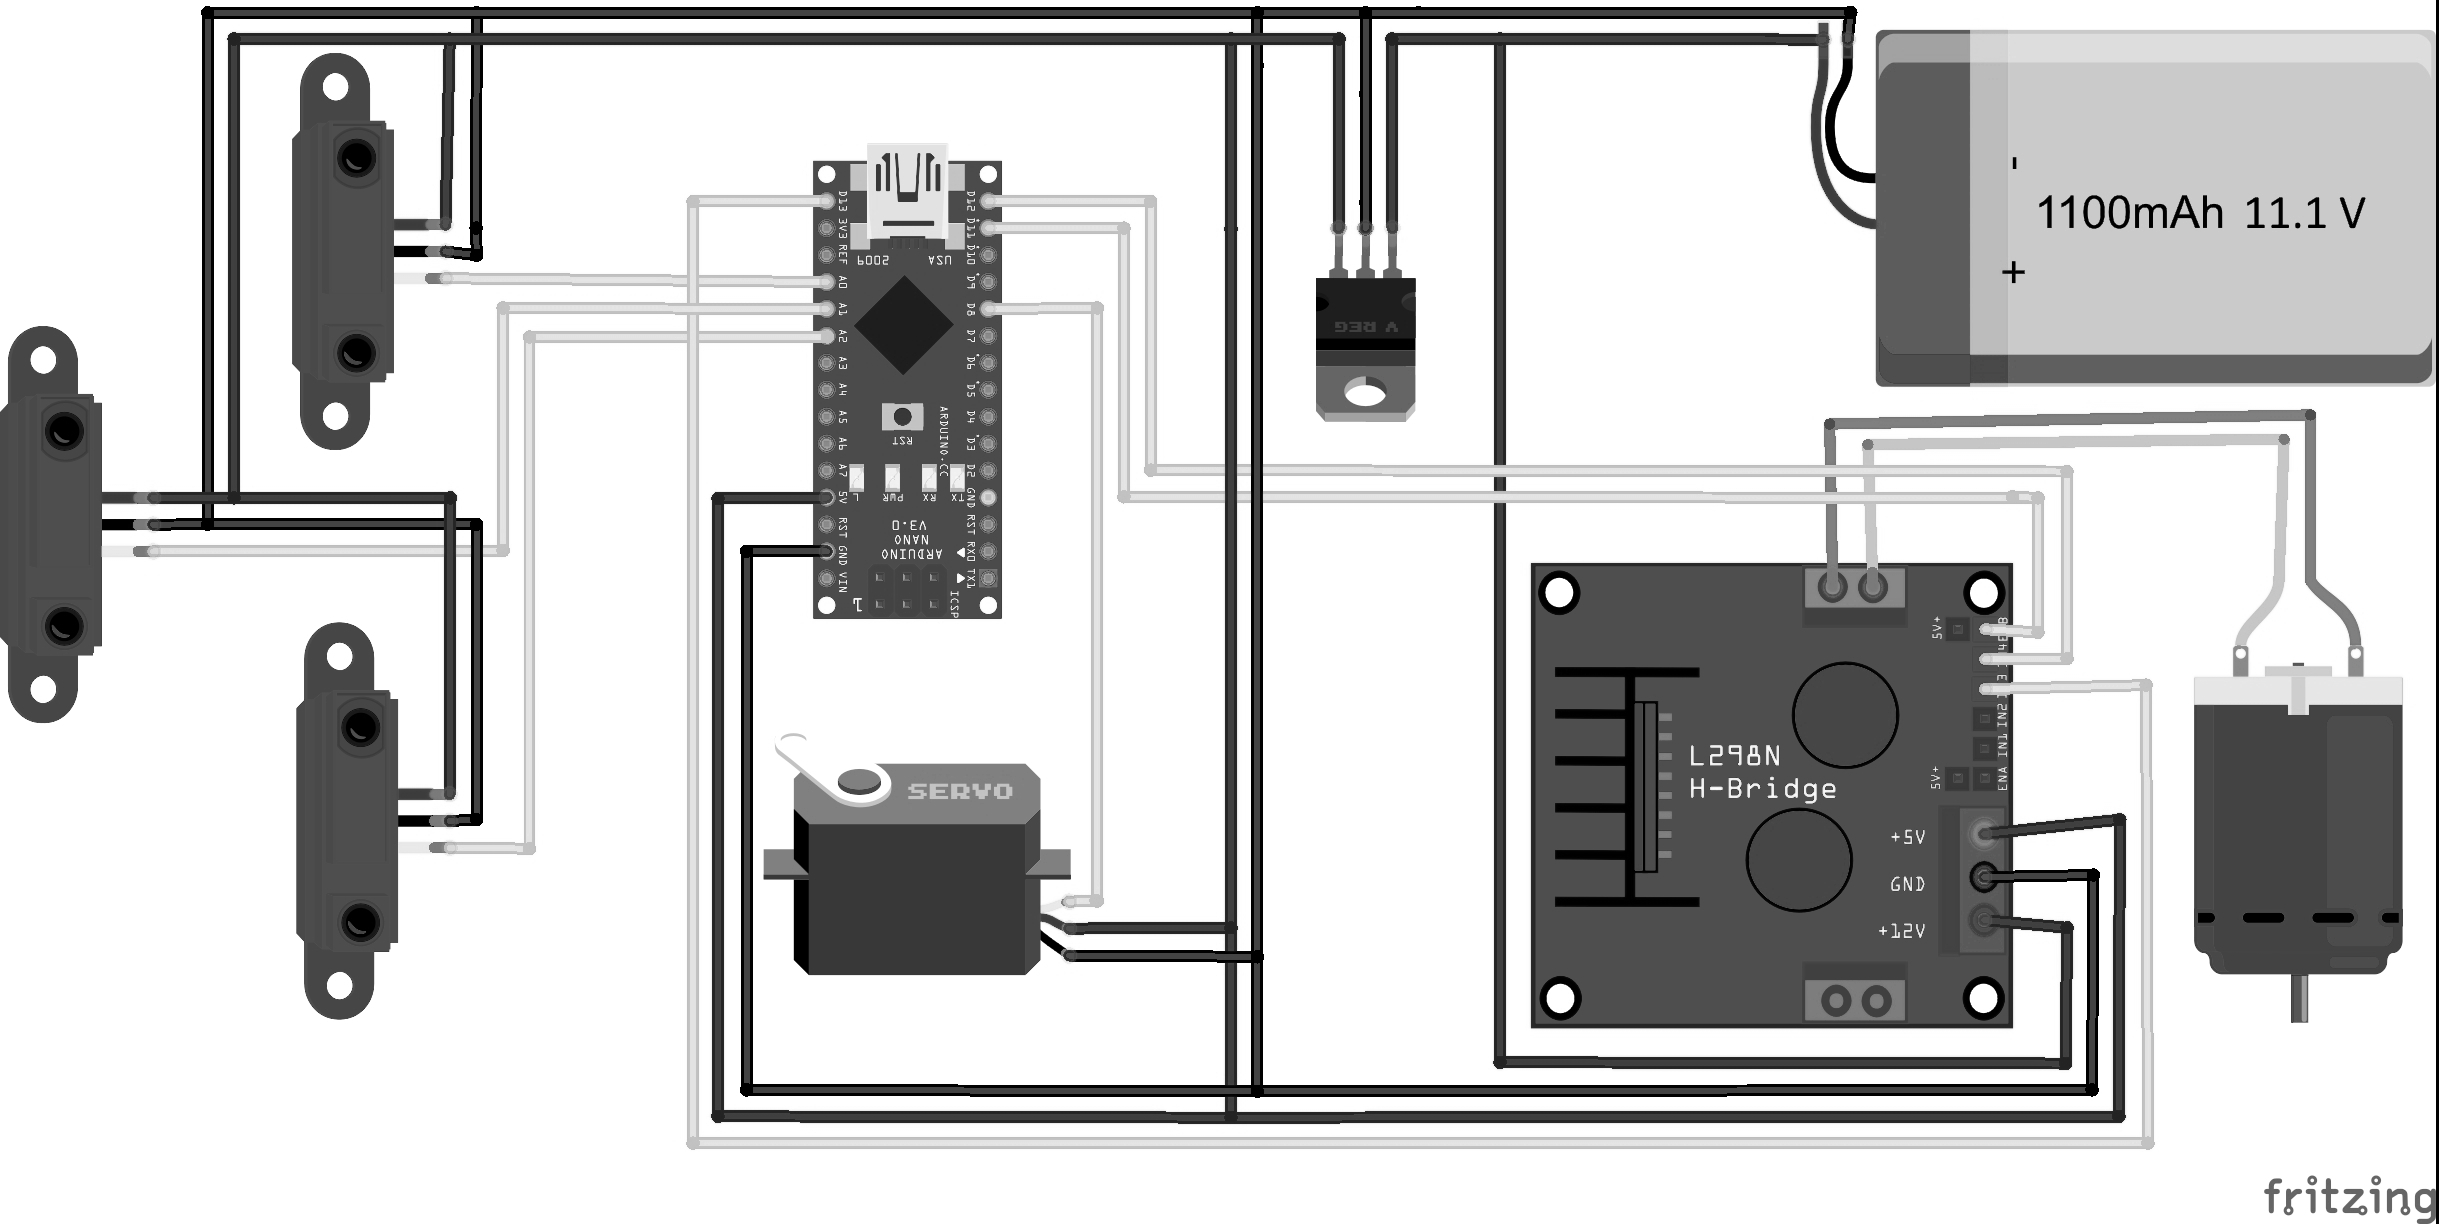
\includegraphics[scale=0.4]{12_2015_fig5}
    \caption{Общая схема робота}\label{sklipus5}
\end{figure}

\subsection*{Программирование робота}

Так как на роботе используется Arduino, то программирование выполняется с использованием Arduino IDE. Программа робота представляет собой замкнутый цикл, который состоит из следующих блоков:

\begin{enumerate}
  \item Фильтрация показаний датчиков;
  \item Вычисление угла и скорости движения робота;
  \item Передача управляющих сигналов на механизмы.
\end{enumerate}

В данной структуре отсутствует блок получения информации от датчиков. Так как датчики возвращают аналоговый сигнал, в Arduino IDE есть функция analogWrite(). Данная функция замечательно работает, если не важна скорость измерения. Но так как робот разрабатывался для соревнований, было принято решение вынести обработку датчиков в прерывание.

Все  платы Arduino, построенные на микроконтроллере ATmega, имеют возможность проводить измерения АЦП в автоматическом режиме. Нужно один раз настроить этот режим, а потом пользоваться полученными значениями. В результате контроллер постоянно проверяет датчики, не тратя на это процессорное время. Фильтрация показаний датчиков осуществляется медианным фильтром с окном в три элемента.

Для движения по трассе был выработан следующий алгоритм. Робот сравнивает расстояния до правой и левой стенки, и в соответствии с этим поворачивает колеса в нужное направление. Если впереди робота нет препятствий, скорость  увеличивается, но также уменьшается максимально возможный угол поворота колес. Это нужно для того, чтобы на прямых участках робот ехал более прямо. При обнаружении препятствия угол поворота колес увеличивается, и робот притормаживает.

Есть конечно и нерешенные проблемы. Например, робот не знает кривизну поворота, поэтому тормозит перед каждым поворотом.

Посмотреть код проекта можно на GitHub \cite{bib3}.

\begin{thebibliography}{9}
\bibitem{bib1} \url{http://en.wikipedia.org/wiki/Servo\_\%28radio\_control\%29}
\bibitem{bib2} \url{http://sites.google.com/site/sklipusrobotsystems/hardware/power-of-robot}
\bibitem{bib3} \url{https://github.com/sklipus/roborace/tree/master/robots/FreshSRDEDITION}\end{thebibliography}
\end{document}

\documentclass[10pt, a5paper]{article}
\usepackage{pdfpages}
\usepackage{parallel}
\usepackage[T2A]{fontenc}
\usepackage{ucs}
\usepackage[utf8x]{inputenc}
\usepackage[polish,english,russian]{babel}
\usepackage{hyperref}
\usepackage{rotating}
\usepackage[inner=2cm,top=1.8cm,outer=2cm,bottom=2.3cm,nohead]{geometry}
\usepackage{listings}
\usepackage{graphicx}
\usepackage{wrapfig}
\usepackage{longtable}
\usepackage{indentfirst}
\usepackage{array}
\newcolumntype{P}[1]{>{\raggedright\arraybackslash}p{#1}}
\frenchspacing
\usepackage{fixltx2e} %text sub- and superscripts
\usepackage{icomma} % коскі ў матэматычным рэжыме
\PreloadUnicodePage{4}

\newcommand{\longpage}{\enlargethispage{\baselineskip}}
\newcommand{\shortpage}{\enlargethispage{-\baselineskip}}

\def\switchlang#1{\expandafter\csname switchlang#1\endcsname}
\def\switchlangbe{
\let\saverefname=\refname%
\def\refname{Літаратура}%
\def\figurename{Іл.}%
}
\def\switchlangen{
\let\saverefname=\refname%
\def\refname{References}%
\def\figurename{Fig.}%
}
\def\switchlangru{
\let\saverefname=\refname%
\let\savefigurename=\figurename%
\def\refname{Литература}%
\def\figurename{Рис.}%
}

\hyphenation{admi-ni-stra-tive}
\hyphenation{ex-pe-ri-ence}
\hyphenation{fle-xi-bi-li-ty}
\hyphenation{Py-thon}
\hyphenation{ma-the-ma-ti-cal}
\hyphenation{re-ported}
\hyphenation{imp-le-menta-tions}
\hyphenation{pro-vides}
\hyphenation{en-gi-neering}
\hyphenation{com-pa-ti-bi-li-ty}
\hyphenation{im-pos-sible}
\hyphenation{desk-top}
\hyphenation{elec-tro-nic}
\hyphenation{com-pa-ny}
\hyphenation{de-ve-lop-ment}
\hyphenation{de-ve-loping}
\hyphenation{de-ve-lop}
\hyphenation{da-ta-ba-se}
\hyphenation{plat-forms}
\hyphenation{or-ga-ni-za-tion}
\hyphenation{pro-gramming}
\hyphenation{in-stru-ments}
\hyphenation{Li-nux}
\hyphenation{sour-ce}
\hyphenation{en-vi-ron-ment}
\hyphenation{Te-le-pathy}
\hyphenation{Li-nux-ov-ka}
\hyphenation{Open-BSD}
\hyphenation{Free-BSD}
\hyphenation{men-ti-on-ed}
\hyphenation{app-li-ca-tion}

\def\progref!#1!{\texttt{#1}}
\renewcommand{\arraystretch}{2} %Іначай формулы ў матрыцы зліпаюцца з лініямі
\usepackage{array}

\def\interview #1 (#2), #3, #4, #5\par{

\section[#1, #3, #4]{#1 -- #3, #4}
\def\qname{LVEE}
\def\aname{#1}
\def\q ##1\par{{\noindent \bf \qname: ##1 }\par}
\def\a{{\noindent \bf \aname: } \def\qname{L}\def\aname{#2}}
}

\def\interview* #1 (#2), #3, #4, #5\par{

\section*{#1\\{\small\rm #3, #4. #5}}

\def\qname{LVEE}
\def\aname{#1}
\def\q ##1\par{{\noindent \bf \qname: ##1 }\par}
\def\a{{\noindent \bf \aname: } \def\qname{L}\def\aname{#2}}
}

\begin{document}
\title{Использование Blender при создании анимационного проекта}
\author{Виктория Бабахина, Рязань, РФ\footnote{\url{vitorry@gmail.com}, \url{http://lvee.org/ru/abstracts/158}}}
\maketitle
\begin{abstract}
The article gives an overview of the free software usage in film"=making industry. It covers all the basic steps of creating an animated film with specifics related to Blender.
\end{abstract}

При работе над анимационным проектом перед художником"=аниматором часто возникает ряд весьма нетривиальных задач. Если речь идет не о крупной студии, то аниматор часто становится и художником по фонам, и моделлером, и компоузером, и даже специалистом по видео"=монтажу. В таких условиях очень важно иметь под рукой удобное программное обеспечение, позволяющее выполнять как можно большее количество задач из разных областей создания готового мультипликата, обладающее при этом достаточной интерактивностью, удобством в обращении и, что весьма важно, адекватной ценой. Здесь мы рассмотрим, как с этой ролью справляется пакет Blender.

\section*{Задачи}

Вот лишь небольшой перечень задач, с которыми может столкнуться в работе художник"=аниматор: создание фонов, моделирование и анимация трехмерных объектов, анимация двухмерных объектов и кривых, создание эффектов,  работа с motion"=графикой, 
композитинг.

\section*{Выбор рендера}

Перед началом работы часто встает вопрос о том, каким рендером пользоваться. Blender предоставляет для работы следующие:

\begin{description}
  \item[Internal.] Рендер, более старый, чем Cycles, не фотореалистичный. Internal "--- это рендер с допущениями. К его несомненным плюсам можно отнести то, что он позволяет рендерить дым, волосы, ночные пейзажи и т. д., при рендере на CPU он значительно быстрее, отлично справляется со стилизованной картинкой, motion"=графикой, стилизацией под 2D и со всем, где не нужен реалистичный рендер. Из минусов "--- больше работы с настройками материалов, рендер с допущениями, и в нем нет глобального освещения и цветных рефлексов.
  \item[Cycles.] Плюсы: фотореалистичный рендер, быстрая и более удобная настройка материалов, просчет на GPU, что более удобно для графики, рендер, удобный для работы с интерьерами. Минусы "--- много проблем с шумом при рендере, трудности с рендером частиц и OSL.
  \item[Freestyle render.] Предназначен для стилизации под 2D"=изображение. 
Freestyle генерирует двумерные линии из набора объектов, линии могут быть стилизованы различными способами (разные цвета и толщины или добавление случайной неровности) для создания художественного (рисунка от руки) или технического (чертёжного) стилей. 
Freestyle может использоваться как дополнение к другим рендерам.
Freestyle для Blender имеет два дополнительных режима для стилизации линий: параметрический редактор и режим Python"=скриптов.
\end{description}

\section*{3D "--- моделинг, риггинг, текстуры, анимация}

Основная функция пакета Blender "--- это работа с 3D"=графикой. При работе над мультипликационным проектом, работа с трехмерной графикой бывает нужна даже в тех случаях, когда речь идет исключительно о 2D"=анимации. К примеру, при создании фонов для упрощения и ускорения рабочего процесса бывает удобно сделать трехмерную модель сцены и рендерить нужные ракурсы при необходимости и в нужном количестве. Для сглаживания разницы между трехмерным фоном и нарисованными плоскими персонажами удобно использовать Freestyle"=рендер, о котором шла речь ранее.

Часто более трудоемким является создание трехмерной модели персонажа. 
Обычные этапы создания трехмерного персонажа выглядят так: 
Подготовительный этап "--- сбор референсов, работа над образом персонажа в эскизах, создание листов персонажа.

\begin{itemize}
  \item Моделирование и текстуры "--- непосредственная работа над моделью.
  \item Риг и лицевой риг "--- оснащение персонажа скелетом и мимикой.
  \item Липсинк "--- создание речевой анимации и фонем.
\end{itemize}

В блендере есть возможность автоматизировать процесс, соответствующий последнему пункту. Для этого необходимо провести подготовительный этап "--- создать шейпы движения губ, соответствующие определенным буквам, и грамотно их переименовать. Затем требуется помощь стороннего приложения для кодирования звука "--- такой например, как Papagayo. В стороннее приложение загружается звуковой файл с текстом, который считывается и кодируется в формат, пригодный для чтения Blender. Результат загружается в Blender, с помощью специального плагина привязывается к модели и автоматически создает ключевые кадры с анимацией.

\section*{2D"=анимация и motion"=графика}

Помимо работы над 3D"=анимацией, Blender располагает обширным инструментарием для работы с 2D"=графикой, который постепенно расширяется и развивается "--- порой в весьма неожиданных направлениях.

Ранее уже было сказано о рендере Freestyle, позволяющем создать имитацию рисованной анимации.  Помимо стилизации во \linebreak Freestyle, в Blender возможна работа над настоящими 2D"=марионетками. С помощью плагина <<Import image as plane>> в блендер загружается персонаж "--- это можно сделать либо по частям, либо и одним изображением, чтобы выполнить его нарезку уже в Blender. Затем марионетка оснащается скелетом и анимируется.

Еще один прием, который способен сильно выручить при работе не только с двумерной анимацией, но и с motion"=графикой "--- это анимация процедурных текстур. С ее помощью сложно получить реалистичные эффекты, какие получились бы при работе с симуляторами огня, дыма или воды; однако когда речь идет о более стилизованной графике,  процедурные текстуры становятся незаменимы. К несомненным плюсам работы с ними относится высокая скорость просчета, отсутствие рывка движения при окончании цикла анимации, возможность сделать анимацию любого размера без потерь качества.

В последнее время появился еще один, весьма неожиданный способ работы с 2D"=анимацией в Blender "--- grease pencil. Изначально это была довольно удобная, но далекая от анимации функция рисования в окне программы. С ее помощью можно было выделить для себя важные моменты при моделировании, наметить траекторию будущей анимации и другие вещи, полезные в работе. И так было до выхода мультипликационного фильма <<For You>>, созданного в технике покадровой анимации исключительно с помощью grease pencil.

\section*{Композитинг}

Изображение, получаемое непосредственно после рендера "--- далеко не финальный результат. Огромное количество работы над изображением ведется на этапе постобработки "--- композитинга.

Финальная картинка при рендере "--- это финальная работа сочетания огромного количества слоев. То есть, даже если не ведется специальная работа над композитингом, он все равно ведется глубоко на уровне кода. В Blender эти слои называются \emph{пассы}.  Пассы позволяют влиять на свет, тени, переотражения, блики, цвета, материалы, маски, глубину и многое другое.

Работа с пассами "--- это не все, что можно осуществить при композитинге. С помощью различных входных нодов возможно, к примеру, заменить фон на изображение, сократив таким образом время рендеринга в разы. Также возможно разделить объекты рендера из одного изображения в разные слои и рендерить по отдельности все или несколько объектов сцены.

Помимо прочего, при композитинге есть возможность работы с масками (когда необходимо убрать, вставить или выделить какую"=то определенную часть изображения), кеингом (замена однотонного яркого фона на что"=то иное), трекингом (определение  местоположения объектов с помощью камеры и последующая работа с полученными точками).

Таким образом, от раннего этапа создания фильма до постобработки Blender будет полезен художнику"=аниматору и, обладая огромным количеством полезных функций, поможет справиться в том числе с довольно сложными и нетривиальными задачами.

\end{document}

\documentclass[10pt, a5paper]{article}
\usepackage{pdfpages}
\usepackage{parallel}
\usepackage[T2A]{fontenc}
\usepackage{ucs}
\usepackage[utf8x]{inputenc}
\usepackage[polish,english,russian]{babel}
\usepackage{hyperref}
\usepackage{rotating}
\usepackage[inner=2cm,top=1.8cm,outer=2cm,bottom=2.3cm,nohead]{geometry}
\usepackage{listings}
\usepackage{graphicx}
\usepackage{wrapfig}
\usepackage{longtable}
\usepackage{indentfirst}
\usepackage{array}
\newcolumntype{P}[1]{>{\raggedright\arraybackslash}p{#1}}
\frenchspacing
\usepackage{fixltx2e} %text sub- and superscripts
\usepackage{icomma} % коскі ў матэматычным рэжыме
\PreloadUnicodePage{4}

\newcommand{\longpage}{\enlargethispage{\baselineskip}}
\newcommand{\shortpage}{\enlargethispage{-\baselineskip}}

\def\switchlang#1{\expandafter\csname switchlang#1\endcsname}
\def\switchlangbe{
\let\saverefname=\refname%
\def\refname{Літаратура}%
\def\figurename{Іл.}%
}
\def\switchlangen{
\let\saverefname=\refname%
\def\refname{References}%
\def\figurename{Fig.}%
}
\def\switchlangru{
\let\saverefname=\refname%
\let\savefigurename=\figurename%
\def\refname{Литература}%
\def\figurename{Рис.}%
}

\hyphenation{admi-ni-stra-tive}
\hyphenation{ex-pe-ri-ence}
\hyphenation{fle-xi-bi-li-ty}
\hyphenation{Py-thon}
\hyphenation{ma-the-ma-ti-cal}
\hyphenation{re-ported}
\hyphenation{imp-le-menta-tions}
\hyphenation{pro-vides}
\hyphenation{en-gi-neering}
\hyphenation{com-pa-ti-bi-li-ty}
\hyphenation{im-pos-sible}
\hyphenation{desk-top}
\hyphenation{elec-tro-nic}
\hyphenation{com-pa-ny}
\hyphenation{de-ve-lop-ment}
\hyphenation{de-ve-loping}
\hyphenation{de-ve-lop}
\hyphenation{da-ta-ba-se}
\hyphenation{plat-forms}
\hyphenation{or-ga-ni-za-tion}
\hyphenation{pro-gramming}
\hyphenation{in-stru-ments}
\hyphenation{Li-nux}
\hyphenation{sour-ce}
\hyphenation{en-vi-ron-ment}
\hyphenation{Te-le-pathy}
\hyphenation{Li-nux-ov-ka}
\hyphenation{Open-BSD}
\hyphenation{Free-BSD}
\hyphenation{men-ti-on-ed}
\hyphenation{app-li-ca-tion}

\def\progref!#1!{\texttt{#1}}
\renewcommand{\arraystretch}{2} %Іначай формулы ў матрыцы зліпаюцца з лініямі
\usepackage{array}

\def\interview #1 (#2), #3, #4, #5\par{

\section[#1, #3, #4]{#1 -- #3, #4}
\def\qname{LVEE}
\def\aname{#1}
\def\q ##1\par{{\noindent \bf \qname: ##1 }\par}
\def\a{{\noindent \bf \aname: } \def\qname{L}\def\aname{#2}}
}

\def\interview* #1 (#2), #3, #4, #5\par{

\section*{#1\\{\small\rm #3, #4. #5}}

\def\qname{LVEE}
\def\aname{#1}
\def\q ##1\par{{\noindent \bf \qname: ##1 }\par}
\def\a{{\noindent \bf \aname: } \def\qname{L}\def\aname{#2}}
}

\begin{document}
\title{Любительская малобюджетная аэрофотосъёмка с использованием свободного программного обеспечения}
\author{Дмитрий Самсонов, Москва, РФ\footnote{\url{samson.samson.samson@gmail.com}, \url{http://lvee.org/ru/abstracts/161}}}
\maketitle
\begin{abstract}
This work concerns some tasks needed for KAP (Kite Aerial Photography) with free/libre software (mostly from Debian \linebreak GNU/Linux). This method was successfully used for taking aerial photos of several open-airs in 2013 and 2014. Nowadays it is very important to have cheap and simple solution. 
\end{abstract}
Иногда возникает необходимость сделать аэрофотосъёмку. Например, на фестивале, проводящемся на открытом воздухе. Свежепостроенные фестивальные объекты могут не попасть на общедоступные спутниковые снимки, поэтому снимать их приходится самостоятельно. В данной работе рассмотрена методика, применявшаяся при аэрофотосъёмке фестивалей <<Пустые Холмы "--- Город Золотой>> осенью 2013 года и <<Фестиваля 17>> летом 2014 года.

Задача состоит в том, чтобы, подняв фотоаппарат на достаточную высоту, сделать серию вертикальных снимков, после чего <<склеить>> их между собой, привязать к местности и привести в удобную для дальнейшей работы форму.

Немаловажна в наше время низкая стоимость как создания, так и эксплуатации решения подобной задачи.

\begin{figure}[h!]
  \centering \label{samsonov1}
  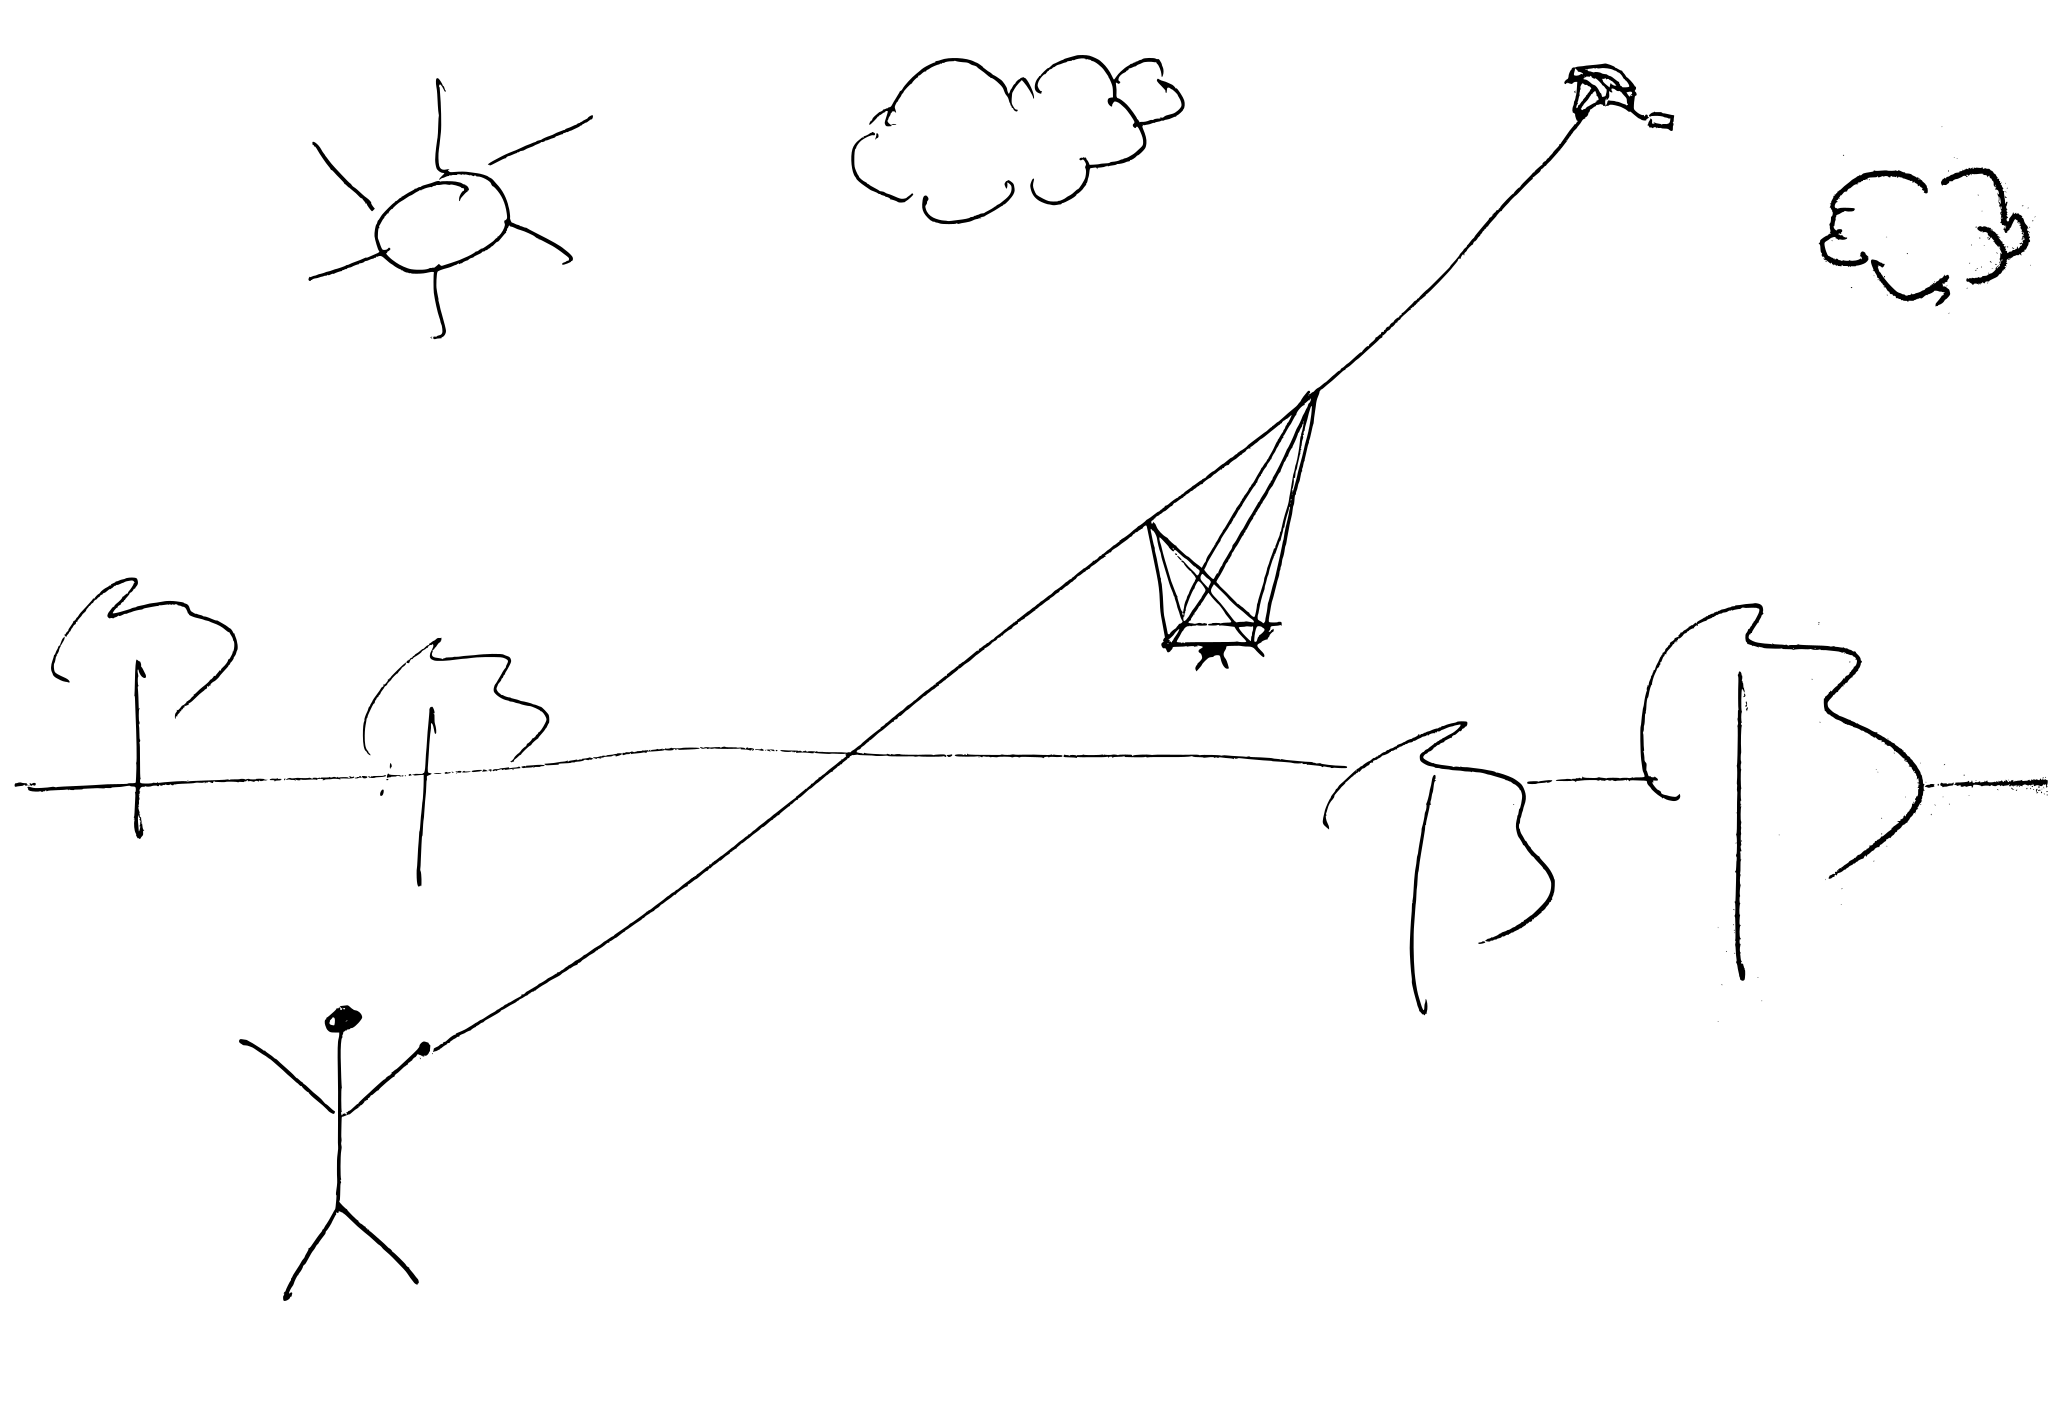
\includegraphics[scale=0.1]{14_2015_fig1}
  \caption{Схематичное изображение процесса аэрофотосъёмки}
\end{figure}


\section*{Аппаратная часть}

Готовые решения в виде специализированных самолётов стоят довольно дорого, а в самостоятельном производстве трудозатратны. Радиоуправляемые вертолёты (<<дроны>>) стоят дешевле, однако дрон, способный устойчиво поднимать в воздух относительно тяжёлый фотоаппарат, стоит существенно дороже дешёвых моделей (а лёгкие фото-видеокамеры дороги сами по себе). К тому же у дронов высокие эксплуатационные издержки. Относительно дешёвы конструкции типа \emph{воздушный змей} и \emph{воздушный шар}. Был выбран первый тип.

Для создания \emph{пикавета} "--- платформы, обеспечивающей вертикальность съёмки "--- была использована часть деревянной коробки, найденная среди бытовых отходов. Крючки для прикрепления пикавета к лееру были найдены в заброшенном цеху НИИДАРа (научно"=исследовательский институт дальней радиосвязи).

\begin{figure}[h!]
  \centering \label{samsonov1}
  \includegraphics[scale=0.1]{14_2015_picavet-color-1}
  \caption{Пикавет}
\end{figure}


Обеспечить серийную съёмку недорогими аппаратами стало возможным благодаря проекту CHDK "--- имеющийся функционал по выполнению скриптов позволил запрограммировать необходимое поведение даже у дешёвой <<мыльницы>> \emph{Canon PowerShot A480}. Отдельным преимуществом является возможность работы от AA"=батареек, что гораздо удобнее в полевых условиях, чем аккумуляторы <<проприетарных>> форматов.

Для привязки к местности снимаются GPS"=координаты нескольких заметных объектов, однако для удешевления можно воспользоваться данными OpenStreetMap и публично доступными спутниковыми снимками. В данном случае использовался \emph{Garmin GPSMAP 62}.

\section*{Программные средства}

Стоит отметить, что почти всё необходимое программное обеспечение (за исключением CHDK) можно обнаружить в дистрибутиве Debian GNU/Linux, что удобно в полевых условиях.

\subsection*{CHDK}

Canon Hacker's Development Kit \cite{samsbib1}, так называемая <<неофициальная прошивка>>, а на самом деле "--- резидентная программа, работающая без модификации прошивки фотоаппарата. Поддерживаются более сотни моделей аппаратов. Позволяет запускать самописные скрипты, программируя логику поведения аппарата в том числе в зависимости от внешних обстоятельств. Для данной задачи оказалось достаточным скрипта для съёмки timelapse, доступного <<из коробки>>.

\subsection*{Hugin}

Hugin \cite{samsbib2} позволяет склеивать фотографии между собой для разных задач. Хотя пакет позиционируется как инструмент для создания круговых панорам, он имеет, наряду с прочими, возможность и <<плоской склейки>>, нужной для данной задачи.

Склейка производится по контрольным точкам. Программа умеет автоматически их находить по похожим участкам изображения, однако на практике склейка проводится в полуавтоматическом режиме "--- требуется ручное вмешательство, как для не очень удачных снимков, так и из"=за параллакса.

Hugin позволяет вычислить точность совмещения снимков, однако за пределами операции склейки в этом мало практического смысла.

\subsection*{QGis}

QGis \cite{samsbib3} "--- геоинформационная система. В нашем случае используется всего лишь для привязки к местности по GPS-точкам (с трансформацией по необходимости) склеенного изображения и получения на выходе изображения в формате GeoTIFF "--- содержащего метаданные о географической привязке.

\subsection*{gdal2tiles}

Для генерации <<тайлов>>, которые могут быть использованы для нужд удобного отображения полученного результата, может быть использован gdal2tiles \cite{samsbib4}.

\subsection*{OpenLayers}

OpenLayers \cite{samsbib5} "--- JavaScript"=библиотека для удобной визуализации через браузер. Впрочем, также можно посоветовать использовать для этих целей Leaflet \cite{samsbib6}.

\section*{Итоги}

\subsection*{Стоимость}

Воздушный змей, способный поднимать несколько килограмм полезной массы (<<грузовой>> или <<лифт>>), стоит чуть больше \$100, но при желании может быть сшит самостоятельно. Важной составляющей является \emph{леер}, километровый моток которого стоит \$50 (выдерживая нагрузку до 40 кг), однако на практике (после одного случая) оказалось более надёжным взять рыболовный шнур <<на сома>> меньшей длины по цене \$30 (выдерживает нагрузку более 100 кг). Платформа для крепления фотоаппарата и мотовило для сматывания леера делаются самостоятельно, хотя при желании на рынке можно найти и готовые решения. Фотоаппарат подойдёт практически любой CHDK"=совместимый, в данном случае использовался \emph{Canon PowerShot A480} (купленный <<с рук>> за \$20), хотя можно было бы достичь лучших результатов с помощью \emph{Canon PowerShot SX20} (купленного <<с рук>> за \$100).

\subsection*{Недостатки и преимущества}

Выбранное решение обладает как рядом существенных недостатков, так и преимуществами.

Для подобного рода задач очевидны проблемы по трудозатратам на ручной отбор удачных снимков и склейку, борьбу с искажениями и параллаксом, зависимость от погодных условий (<<нелётная погода>> при сильном ветре), проблемы безопасности находящихся под камерой людей. Для воздушного змея также характерна неполная управляемость и требования по силе ветра для старта: например, для использованного змея скорость ветра для успешного запуска должна превышать 3 м/с. Также необходимо соблюдать паритет между противоречивыми требованиями длины леера, его прочностью и весом, грузоподъёмностью воздушного змея и требованиями по минимальной скорости ветра для старта.

Попытки запуска с велосипеда при отсутствии естественного ветра не увенчались успехом "--- достичь высоты, необходимой для стабильного полёта, не удалось. Возможно, подобная задача требует конструктивного усовершенствования.

Ограничением также является необходимость открытого пространства для запуска и сложность в перемещении среди препятствий.

Также стоит отметить практическую сложность оценки погрешности точности определения местоположения каждой конкретной точки снимка при данном подходе, однако это приемлемо для любительской съёмки.

С другой стороны, использование воздушного змея позволяет, при удачном стечении обстоятельств, поднять его на высоту, где он может находиться неограниченно долго, пока позволяют погодные условия "--- в любое время суток, даже при отсутствии ветра у поверхности земли. Что позволяет его использовать для постоянного <<лифта>> не только для аэрофотосъёмки, но и для обеспечения мобильной связи в тех случаях, когда у поверхности земли она затруднена (на площадке размещается смартфон, а при необходимости поднять его повыше "--- также и мобильный роутер).

\subsection*{Применение}

Полученную аэрофотосъёмку можно использовать не только в эстетических целях, но и для нужд любительского картографирования, а также в качестве базы для других проектов: например, можно отображать на карте фотографии, сделанные посетителями конкретного мероприятия "--- использование реалистичной подложки упрощает восприятие информации.

\subsection*{Перспективы дальнейшего усовершенствования \linebreak метода}

Для нивелирования некоторых недостатков погодных условий (отсутствие ветра для запуска) можно рассмотреть вопрос использования воздушного шара (BAP "--- Balloon Aerial Photography: чёрный воздушный шар, поднимающийся за счёт нагрева солнечными лучами воздуха внутри него) или применение более лёгкого воздушного змея, который может быть использован в качестве <<лифта>> для основного змея после поднятия на достаточную высоту для стабильного полёта.

\begin{thebibliography}{9}
\bibitem{samsbib1} \url{http://chdk.clan.su/}
\bibitem{samsbib2} \url{http://hugin.sourceforge.net/}
\bibitem{samsbib3} \url{http://qgis.org/ru/site/}
\bibitem{samsbib4} \url{http://www.gdal.org/gdal2tiles.html}
\bibitem{samsbib5} \url{http://openlayers.org/}
\bibitem{samsbib6} \url{http://leafletjs.com/}\end{thebibliography}
\end{document}

\documentclass[10pt, a5paper]{article}
\usepackage{pdfpages}
\usepackage{parallel}
\usepackage[T2A]{fontenc}
\usepackage{ucs}
\usepackage[utf8x]{inputenc}
\usepackage[polish,english,russian]{babel}
\usepackage{hyperref}
\usepackage{rotating}
\usepackage[inner=2cm,top=1.8cm,outer=2cm,bottom=2.3cm,nohead]{geometry}
\usepackage{listings}
\usepackage{graphicx}
\usepackage{wrapfig}
\usepackage{longtable}
\usepackage{indentfirst}
\usepackage{array}
\newcolumntype{P}[1]{>{\raggedright\arraybackslash}p{#1}}
\frenchspacing
\usepackage{fixltx2e} %text sub- and superscripts
\usepackage{icomma} % коскі ў матэматычным рэжыме
\PreloadUnicodePage{4}

\newcommand{\longpage}{\enlargethispage{\baselineskip}}
\newcommand{\shortpage}{\enlargethispage{-\baselineskip}}

\def\switchlang#1{\expandafter\csname switchlang#1\endcsname}
\def\switchlangbe{
\let\saverefname=\refname%
\def\refname{Літаратура}%
\def\figurename{Іл.}%
}
\def\switchlangen{
\let\saverefname=\refname%
\def\refname{References}%
\def\figurename{Fig.}%
}
\def\switchlangru{
\let\saverefname=\refname%
\let\savefigurename=\figurename%
\def\refname{Литература}%
\def\figurename{Рис.}%
}

\hyphenation{admi-ni-stra-tive}
\hyphenation{ex-pe-ri-ence}
\hyphenation{fle-xi-bi-li-ty}
\hyphenation{Py-thon}
\hyphenation{ma-the-ma-ti-cal}
\hyphenation{re-ported}
\hyphenation{imp-le-menta-tions}
\hyphenation{pro-vides}
\hyphenation{en-gi-neering}
\hyphenation{com-pa-ti-bi-li-ty}
\hyphenation{im-pos-sible}
\hyphenation{desk-top}
\hyphenation{elec-tro-nic}
\hyphenation{com-pa-ny}
\hyphenation{de-ve-lop-ment}
\hyphenation{de-ve-loping}
\hyphenation{de-ve-lop}
\hyphenation{da-ta-ba-se}
\hyphenation{plat-forms}
\hyphenation{or-ga-ni-za-tion}
\hyphenation{pro-gramming}
\hyphenation{in-stru-ments}
\hyphenation{Li-nux}
\hyphenation{sour-ce}
\hyphenation{en-vi-ron-ment}
\hyphenation{Te-le-pathy}
\hyphenation{Li-nux-ov-ka}
\hyphenation{Open-BSD}
\hyphenation{Free-BSD}
\hyphenation{men-ti-on-ed}
\hyphenation{app-li-ca-tion}

\def\progref!#1!{\texttt{#1}}
\renewcommand{\arraystretch}{2} %Іначай формулы ў матрыцы зліпаюцца з лініямі
\usepackage{array}

\def\interview #1 (#2), #3, #4, #5\par{

\section[#1, #3, #4]{#1 -- #3, #4}
\def\qname{LVEE}
\def\aname{#1}
\def\q ##1\par{{\noindent \bf \qname: ##1 }\par}
\def\a{{\noindent \bf \aname: } \def\qname{L}\def\aname{#2}}
}

\def\interview* #1 (#2), #3, #4, #5\par{

\section*{#1\\{\small\rm #3, #4. #5}}

\def\qname{LVEE}
\def\aname{#1}
\def\q ##1\par{{\noindent \bf \qname: ##1 }\par}
\def\a{{\noindent \bf \aname: } \def\qname{L}\def\aname{#2}}
}

\begin{document}
\title{Кратко о SO\_BUSY\_POLL}
\author{Евгений Рыбак, Минск, Беларусь\footnote{\url{engler@tut.by}, \url{http://lvee.org/en/abstracts/156}}}
\maketitle
\begin{abstract}
Performance of Linux network stack was always kept in mind during any implementation. Increasing demand for cloud services, multimedia content, high performance computing forces to search new ways of optimization. SO\_BUSY\_POLL is one of the way to improve processing of incoming network messages without changing source code of the product.
\end{abstract}
\subsubsection*{Введение}

Оптимизация скорости обработки входящих пакетов всегда была одной из главных задач сетевого стека. Рост облачных сервисов, объемов мультимедийного контента, высокопроизводительных систем (HPC) заставляет выискивать новые резервы для оптимизаций. SO\_BUSY\_POLL является еще одним способом улучшить производительность системы, практически не меняя исходный текст продукта.

\subsubsection*{Уровни стека TCP/IP}

Как известно, стек TCP/IP состоит из уровней, каждый из которых решает четко поставленную задачу.


\begin{figure}[h!]
  \centering 
  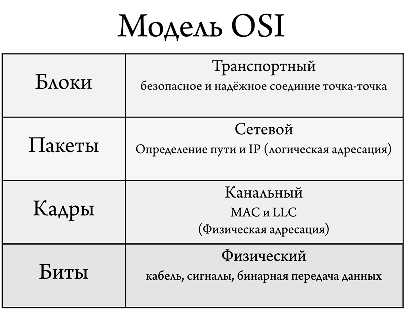
\includegraphics[scale=0.6]{15_2015_Osi-model-50}
\end{figure}


Физический уровень отвечает за передачу и прием электрических данных по сетевому кабелю, в соответствии с методами кодирования.

Канальный уровень отвечает за преобразование из электрического сигнала в цифровой кадр, аппаратную адресацию (MAC"=адрес).

Сетевой уровень отвечает за связывание отдельных подсетей, в целую сеть. Идентификация узла в сети осуществляется с помощью IP"=адреса.

Транспортный уровень отвечает за идентификацию процесса, в рамках узла, которому необходимо передать данные. Идентификация процесса осуществляется с помощью номера порта.

\subsubsection*{Методы обработки входящих пакетов}

Классически, есть два основных подхода для того, что бы узнать, что на сетевой адаптер пришли новые пакеты:

\begin{itemize}
  \item метод прерываний (IRQ);
  \item метод опроса (polling).
\end{itemize}

Каждый из методов имеет свои достоинства и недостатки: метод прерываний хорошо себя показал для небольшого объема трафика, когда прерывания генерируются не часто, не мешая процессору выполнять свои задачи. В случае большого и очень большого объема трафика метод является не очень эффективным; именно в этом случае метод опроса устройства является наиболее подходящим. Busy Poll (новая опция SO\_BUSY\_POLL) является усовершенствованием классического метода опроса, который уменьшает задержку (Latency) и увеличивает пропускную способность (Throughput).

\subsubsection*{Обзор опции SO\_BUSY\_POLL}

Начиная с версии ядра 3.11, ядро осуществляет поддержку опции сокета SO\_BUSY\_POLL.
В эко"=системе SO\_BUSY\_POLL \linebreak участвуют следующие компоненты:

\begin{itemize}
  \item ядро операционной системы;
  \item драйвер сетевой карты;
  \item настройки системы.
\end{itemize}

\textit{Поддержка ядра операционной системы}

Ядро должно быть собрано с опцией \linebreak CONFIG\_NET\_RX\_BUSY\_POLL.

\textit{Драйвер сетевой карты}

Драйвер сетевой карты должен реализовать обработчик функции, который отвечает за busy polling.

\textit{Настройки системы}

В сетевых настройках появились две новые опции: busy\_read, busy\_poll.
Значением является количество микросекунд, в течении которого ядро будет опрашивать входящую очередь сетевой карты (Ethernet RX queue).
Прочитать и записать значения можно следующим образом:

\begin{verbatim}
sysctl net.core.busy_read 
sysctl net.core.busy_poll
sysctl net.core.busy_read=50
sysctl net.core.busy_poll=50
\end{verbatim}

Также рассмотрим влияние опции SO\_BUSY\_POLL на различные методы чтения TCP/UDP"=сокетов.

\subsubsection*{Отличие busy poll от NAPI poll}

\begin{figure}[h!]
  \centering 
  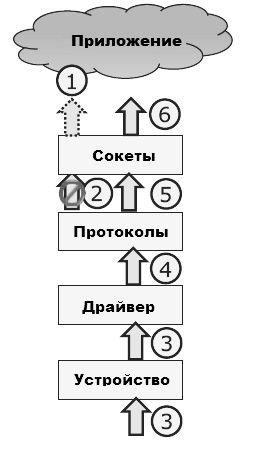
\includegraphics[scale=0.6]{15_2015_classic-packet-path-wo-busy-poll-ru}
\end{figure}

На рисунке выше показана работа приложения с точки зрения \linebreak NAPI poll. Схема включает следующие этапы:

\begin{enumerate}
  \item Приложение создает сокет и пытается из него прочитать данные.
  \item Данные отсутствуют, ожидаем момент, когда они появятся в буфере сокета.
  \item Данные приходят на интерфейс.
  \item Генерируется прерывание, данные передаются на уровень протоколов.
  \item Данные передаются в буфер сокета.
  \item Приложение может прочитать данные из сокета.
\end{enumerate}

В отличие от предыдущей, схема работы с включенной опцией SO\_BUSY\_POLL выглядит так:

\begin{figure}[h!]
  \centering 
  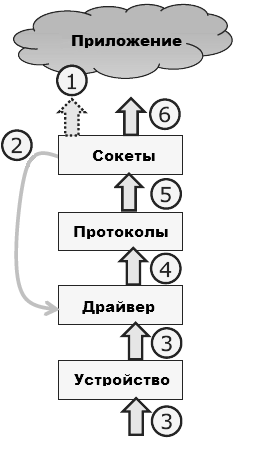
\includegraphics[scale=0.6]{15_2015_classic-packet-path-with-busy-poll-ru}
\end{figure}


\begin{enumerate}
  \item Приложение создает сокет и пытается из него прочитать данные.
  \item Если данных в буфере сокета нету, переходим к функции драйвера busy poll.
  \item Данные приходят на интерфейс.
  \item Генерируется прерывание, данные передаются на уровень протоколов.
  \item Данные передаются в буфер сокета.
  \item Приложение может прочитать данные из сокета.
\end{enumerate}

Одна из отличительных возможностей busy poll заключается в том, что если данные в буфере сокета отсутствуют, то нам не надо ждать прерывания от драйвера сетевой карты, как в случае с NAPI poll. Busy poll инициирует «принудительную» передачу пакетов из входящей очереди драйвера в очередь сокета, тем самым исключая «лишнее» переключение контекста и прерывание.

Еще одним моментом, на который стоит обратить внимание, является то, что в случае обработчика NAPI poll система передает количество пакетов, которое она готова обработать в данный момент. Если количество пакетов в очереди драйвера больше, чем количество пакетов, которое система готова обработать в текущий момент, то обработчик NAPI poll будет еще раз поставлен в очередь вызовов; через некоторый промежуток времени обработчик будет вызван в очередной раз.

В случае с busy poll, обработчик busy polling будет вызываться в течении времени, которое будет указано в опции SO\_BUSY\_POLL или настройках busy\_\{read,poll\}

\subsubsection*{Источники}

\begin{thebibliography}{9}
  \bibitem{sdf1} {A way towards Lower Latency and Jitter.} \url{http://www.linuxplumbersconf.org/2012/wp-content/uploads/2012/09/2012-lpc-Low-Latency-Sockets-slides-brandeburg.pdf}
  \bibitem{sdf2} {Open Source Kernel Enhancements for Low Latency Socket.} \url{http://www.intel.com/content/dam/www/public/us/en/documents/white-papers/open-source-kernel-enhancements-paper.pdf}
  \bibitem{sdf3} {Net: low latency Ethernet device polling.} \url{https://lwn.net/Articles/540281/}
  \bibitem{sdf4} {Understanding Linux Network Internals.} \url{http://www.amazon.com/Understanding-Network-Internals-Christian-Benvenuti/dp/0596002556}
  \bibitem{sdf5} {Linux Kernel Development.} \url{http://www.amazon.com/Linux-Kernel-Development-Robert-Love/dp/0672329468/ref=sr_1_1?s=books&ie=UTF8&qid=1434287714&sr=1-1&keywords=Linux.Kernel.Development}
  \bibitem{sdf6} {Linux Kernel Sources 3.18.14.} \url{https://www.kernel.org/pub/linux/kernel/v3.x/linux-3.18.14.tar.gz}
\end{thebibliography}
\end{document}

\documentclass[10pt, a5paper]{article}
\usepackage{pdfpages}
\usepackage{parallel}
\usepackage[T2A]{fontenc}
\usepackage{ucs}
\usepackage[utf8x]{inputenc}
\usepackage[polish,english,russian]{babel}
\usepackage{hyperref}
\usepackage{rotating}
\usepackage[inner=2cm,top=1.8cm,outer=2cm,bottom=2.3cm,nohead]{geometry}
\usepackage{listings}
\usepackage{graphicx}
\usepackage{wrapfig}
\usepackage{longtable}
\usepackage{indentfirst}
\usepackage{array}
\newcolumntype{P}[1]{>{\raggedright\arraybackslash}p{#1}}
\frenchspacing
\usepackage{fixltx2e} %text sub- and superscripts
\usepackage{icomma} % коскі ў матэматычным рэжыме
\PreloadUnicodePage{4}

\newcommand{\longpage}{\enlargethispage{\baselineskip}}
\newcommand{\shortpage}{\enlargethispage{-\baselineskip}}

\def\switchlang#1{\expandafter\csname switchlang#1\endcsname}
\def\switchlangbe{
\let\saverefname=\refname%
\def\refname{Літаратура}%
\def\figurename{Іл.}%
}
\def\switchlangen{
\let\saverefname=\refname%
\def\refname{References}%
\def\figurename{Fig.}%
}
\def\switchlangru{
\let\saverefname=\refname%
\let\savefigurename=\figurename%
\def\refname{Литература}%
\def\figurename{Рис.}%
}

\hyphenation{admi-ni-stra-tive}
\hyphenation{ex-pe-ri-ence}
\hyphenation{fle-xi-bi-li-ty}
\hyphenation{Py-thon}
\hyphenation{ma-the-ma-ti-cal}
\hyphenation{re-ported}
\hyphenation{imp-le-menta-tions}
\hyphenation{pro-vides}
\hyphenation{en-gi-neering}
\hyphenation{com-pa-ti-bi-li-ty}
\hyphenation{im-pos-sible}
\hyphenation{desk-top}
\hyphenation{elec-tro-nic}
\hyphenation{com-pa-ny}
\hyphenation{de-ve-lop-ment}
\hyphenation{de-ve-loping}
\hyphenation{de-ve-lop}
\hyphenation{da-ta-ba-se}
\hyphenation{plat-forms}
\hyphenation{or-ga-ni-za-tion}
\hyphenation{pro-gramming}
\hyphenation{in-stru-ments}
\hyphenation{Li-nux}
\hyphenation{sour-ce}
\hyphenation{en-vi-ron-ment}
\hyphenation{Te-le-pathy}
\hyphenation{Li-nux-ov-ka}
\hyphenation{Open-BSD}
\hyphenation{Free-BSD}
\hyphenation{men-ti-on-ed}
\hyphenation{app-li-ca-tion}

\def\progref!#1!{\texttt{#1}}
\renewcommand{\arraystretch}{2} %Іначай формулы ў матрыцы зліпаюцца з лініямі
\usepackage{array}

\def\interview #1 (#2), #3, #4, #5\par{

\section[#1, #3, #4]{#1 -- #3, #4}
\def\qname{LVEE}
\def\aname{#1}
\def\q ##1\par{{\noindent \bf \qname: ##1 }\par}
\def\a{{\noindent \bf \aname: } \def\qname{L}\def\aname{#2}}
}

\def\interview* #1 (#2), #3, #4, #5\par{

\section*{#1\\{\small\rm #3, #4. #5}}

\def\qname{LVEE}
\def\aname{#1}
\def\q ##1\par{{\noindent \bf \qname: ##1 }\par}
\def\a{{\noindent \bf \aname: } \def\qname{L}\def\aname{#2}}
}

\begin{document}
\title{Data Science for Network Security}
\author{Dmitry Orekhov, Minsk, Belarus\footnote{\url{Dmitry_Orekhov@epam.com}, \url{http://lvee.org/en/abstracts/164}}}
\maketitle
\begin{abstract}
Today network traffic is absolutely out of human control, this is something that human mind cannot manage. On the other hand, network security becomes more and more important, since more and more of human activities are moving to the Network.
The solution could be a software, which is able to learn from past Data incoming, and then to make assumptions about new Data and predictions about the future. Though algorithms for this domain are well-known, there is a problem to implement them, because they are often very resource-consuming. Fortunately, cloud technologies now afford building cheap and productive clusters, and Open Source solutions like Spark provide a powerful tool to build advanced analytics software on top of them.
\end{abstract}
\subsection*{Data collecting}

The first important task for Network Analytics building is a data collection facility. The main idea is to place sensors, which collect statistics data and send it to be collect and analyze.

\begin{figure}[h!]
  \centering 
  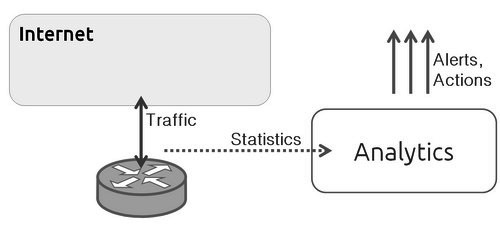
\includegraphics[scale=0.5]{16_2015_fig1}
  
  Fig.1: Statistics collection: the big picture
\end{figure}

\subsubsection*{Sensors}

Sensors are classified by Vantage and Domain. 
\textbf{Vantage} is a place\-ment of sensors within a network. Sensors with different vantages would see different parts of the same events.
\begin{figure}[h!]
  \centering 
  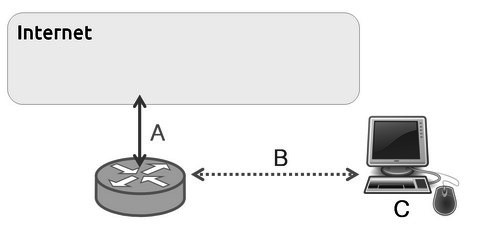
\includegraphics[scale=0.5]{16_2015_fig2}
    
  Fig.2: Vantages
\end{figure}

\textbf{Domain} defines which part of thraffic statistics and metrics to collect. In the other words, it's the information the sensor provides, whether that’s at the host, a service on the host, or the network. Sensors with the same vantage but different domains provide complementary data about the same event. For some events, you might only get informa\-tion from one domain.
\begin{figure}[h!]
  \centering 
  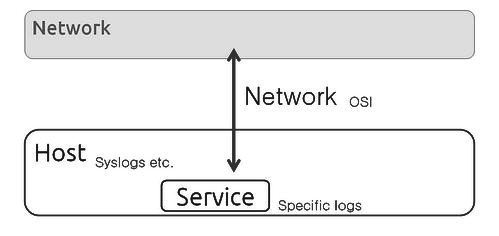
\includegraphics[scale=0.5]{16_2015_fig3}
    
  Fig.3: Domains
\end{figure}

\subsection*{Use Case: DNS Tunneling}

Tunneling -- a mechaninsm to encapsulate low-lewel protocols into high-level protocol.
\begin{figure}[h!]
  \centering 
  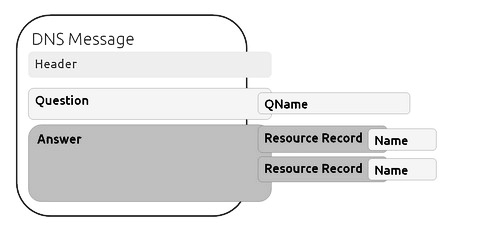
\includegraphics[scale=0.8]{16_2015_fig4}
    
  Fig.4: DNS message, a Big Picture
\end{figure}

In case of DNS tunneling, DNS Resource Records so as Questions may contain Canonical Names; these Names can be easily encoded/de\-coded with Base32 or Base64 methods and can be used to transport unauthorized traffic or botnet protocol commands.

\begin{figure}[h!]
  \centering 
  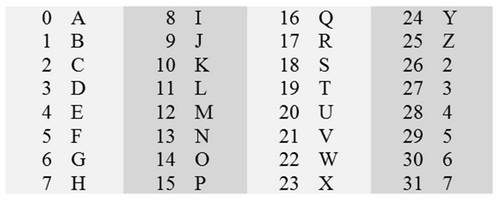
\includegraphics[scale=0.8]{16_2015_fig5}
    
  Fig.5: Base32 encoding
\end{figure}


\subsubsection*{Methods to discover}

\textbf{Payload analysis}

\begin{itemize}
  \item Size of request and response
  \item Entropy of hostnames
  \item Statistical Analysis
  \item Uncommon Record Types
\end{itemize}

\textbf{Traffic analysis}

\begin{itemize}
  \item Volume of DNS traffic per IP address
  \item Volume of DNS traffic per domain
  \item Number of hostnames per domain
  \item Geographic location of DNS server
  \item Domain history
  \item Orphan DNS requests
\end{itemize}

The problem is that the most effective methods to discover DNS traffic demands deep packet inspection. Also, in case of models  based on long-term history, we have to store much statistical data and re-compile the intrusion detection model in a batch job, to be up-to-date.

\subsubsection*{Algorithms}

All algorithms, which could be used for DNS discovering, realate to Machine Learning area; the domain of it is building system, which can be learnt from Data sets and then make predictions about future trends. Today this is very important part of Data Science.

\paragraph{Online algorithms.}

It start with an initial state and analyze each piece of data serially one at a time.

\begin{itemize}
  \item Generally require a chain of Map Reduce jobs
  \item Good fit for Apache Spark, Storm
  \item Primarily batch, good for Lambda architectures
\end{itemize}

\textbf{Example 1: Outlier detection}

\begin{itemize}
  \item Median Absolute Deviation: Telemetry is anomalous if the \linebreak deviation of its latest datapoint
with respect to the median is X times larger than the median of deviations
  \item Standard Deviation from Average: Telemetry is anomalous if the absolute value of the average of the latest three datapoint minus the moving average is greater than three standard deviations of the average.
  \item Standard Deviation from Moving Average: Telemetry is anomalous if the absolute value of the average of the latest three datapoints minus the moving average is greater than three standard deviati\-ons of the moving average.
  \item Mean Subtraction Cumulation: Telemetry is anomalous if the value of the next datapoint in the series is farther than three standard deviations out in cumulative terms after subtracting the mean from each data point
  \item Least Squares: Telemetry is anomalous if the average of the last three datapoints on a projected least squares model is greater than three sigma
  \item Histogram Bins: Telemetry is anomalous if the average of the last three datapoints falls into a histogram bin with less than x
\end{itemize}

\textbf{Example 2: Stream Classification}

\begin{itemize}
  \item Hoeffding Tree (VFDT)
incremental, anytime decision tree \linebreak induction algorithm that is capable of learning from massive data streams, assuming that the distribution generating examples does not change over time
  \item Half-Space Trees
ensemble model that randomly spits data into half spaces. They are created online and detect anomalies by their deviations in placement within the forest relative to other data from the same window
\end{itemize}

The possible topology Big Picture could be like this:
\begin{figure}[h!]
  \centering 
  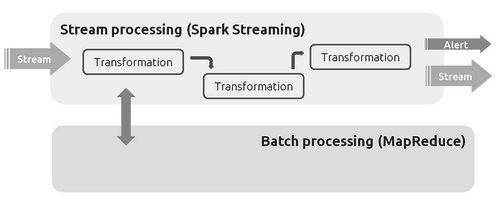
\includegraphics[scale=0.8]{16_2015_fig6}
    
  Fig.6: Online algorithms, Topology
\end{figure}

\paragraph{Offline algorithms.}

It analyzes entire data set at once.

\begin{itemize}
  \item Generally a good fit for Apache Hadoop/Map Reduce
  \item Model compiled via batch, scored via stream processor
\end{itemize}

\textbf{Example: Hypothesis Tests}

\begin{itemize}
  \item Chi2 Test (Goodness of Fit): A feature is anomalous if the data for the latest micro batch (for the last 10 minutes) comes
from a different distribution than the historical distribution for that feature
  \item Grubbs Test: telemetry is anomalous if Z score is greater than the Grubb's score.
  \item Kolmogorov-Smirnov Test: check if data distribution for last 10 minutes is different from last hour
  \item Simple Outliers test: telemetry is anomalous if the number of outliers for the last 10 minutes is statistically different then the
historical number of outliers for that time frame
\end{itemize}

Also, some other types of algorithms can be used

\begin{itemize}
  \item Decision Trees/Random Forests
  \item Association Rules (Apriori)
  \item Auto Regressive (AR) Moving Average (MA)
\end{itemize}

In fact, at using Offlimne algorithms, all analysis is performed as batch tasks, the Streaming part just applies rules compiled by the Batch part. A possible topology Big Picture could be like this
\begin{figure}[h!]
  \centering 
  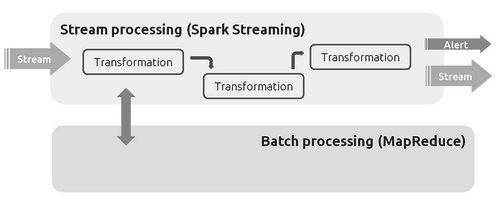
\includegraphics[scale=0.8]{16_2015_fig7}
  
  Fig. 7: Offline algorithms, Topology
\end{figure}

\subsubsection*{Technology stack: everything Free}

It's very important, that all software to build Analytics based on Machine Learning so as for Data storage is Free/Libre one. All solutions which we are using are publiched under Apache 2.0, MIT and so on.
For Streaming part it was used Spark Streaming and Spark for Batch jobs as well. Message Queues which we are using are Kafka and RabbitMQ.

\end{document}

\documentclass[10pt, a5paper]{article}
\usepackage{pdfpages}
\usepackage{parallel}
\usepackage[T2A]{fontenc}
\usepackage{ucs}
\usepackage[utf8x]{inputenc}
\usepackage[polish,english,russian]{babel}
\usepackage{hyperref}
\usepackage{rotating}
\usepackage[inner=2cm,top=1.8cm,outer=2cm,bottom=2.3cm,nohead]{geometry}
\usepackage{listings}
\usepackage{graphicx}
\usepackage{wrapfig}
\usepackage{longtable}
\usepackage{indentfirst}
\usepackage{array}
\newcolumntype{P}[1]{>{\raggedright\arraybackslash}p{#1}}
\frenchspacing
\usepackage{fixltx2e} %text sub- and superscripts
\usepackage{icomma} % коскі ў матэматычным рэжыме
\PreloadUnicodePage{4}

\newcommand{\longpage}{\enlargethispage{\baselineskip}}
\newcommand{\shortpage}{\enlargethispage{-\baselineskip}}

\def\switchlang#1{\expandafter\csname switchlang#1\endcsname}
\def\switchlangbe{
\let\saverefname=\refname%
\def\refname{Літаратура}%
\def\figurename{Іл.}%
}
\def\switchlangen{
\let\saverefname=\refname%
\def\refname{References}%
\def\figurename{Fig.}%
}
\def\switchlangru{
\let\saverefname=\refname%
\let\savefigurename=\figurename%
\def\refname{Литература}%
\def\figurename{Рис.}%
}

\hyphenation{admi-ni-stra-tive}
\hyphenation{ex-pe-ri-ence}
\hyphenation{fle-xi-bi-li-ty}
\hyphenation{Py-thon}
\hyphenation{ma-the-ma-ti-cal}
\hyphenation{re-ported}
\hyphenation{imp-le-menta-tions}
\hyphenation{pro-vides}
\hyphenation{en-gi-neering}
\hyphenation{com-pa-ti-bi-li-ty}
\hyphenation{im-pos-sible}
\hyphenation{desk-top}
\hyphenation{elec-tro-nic}
\hyphenation{com-pa-ny}
\hyphenation{de-ve-lop-ment}
\hyphenation{de-ve-loping}
\hyphenation{de-ve-lop}
\hyphenation{da-ta-ba-se}
\hyphenation{plat-forms}
\hyphenation{or-ga-ni-za-tion}
\hyphenation{pro-gramming}
\hyphenation{in-stru-ments}
\hyphenation{Li-nux}
\hyphenation{sour-ce}
\hyphenation{en-vi-ron-ment}
\hyphenation{Te-le-pathy}
\hyphenation{Li-nux-ov-ka}
\hyphenation{Open-BSD}
\hyphenation{Free-BSD}
\hyphenation{men-ti-on-ed}
\hyphenation{app-li-ca-tion}

\def\progref!#1!{\texttt{#1}}
\renewcommand{\arraystretch}{2} %Іначай формулы ў матрыцы зліпаюцца з лініямі
\usepackage{array}

\def\interview #1 (#2), #3, #4, #5\par{

\section[#1, #3, #4]{#1 -- #3, #4}
\def\qname{LVEE}
\def\aname{#1}
\def\q ##1\par{{\noindent \bf \qname: ##1 }\par}
\def\a{{\noindent \bf \aname: } \def\qname{L}\def\aname{#2}}
}

\def\interview* #1 (#2), #3, #4, #5\par{

\section*{#1\\{\small\rm #3, #4. #5}}

\def\qname{LVEE}
\def\aname{#1}
\def\q ##1\par{{\noindent \bf \qname: ##1 }\par}
\def\a{{\noindent \bf \aname: } \def\qname{L}\def\aname{#2}}
}

\begin{document}
\title{История одного маленького дистрибутива Linux}
\author{Денис Пынькин, Минск, Беларусь\footnote{\url{denis_pynkin@epam.com}, \url{http://lvee.org/en/abstracts/167}}}
\maketitle
\begin{abstract}
Article presents the creation and support history of the Linux-based infrastructure in ECM department of BSUIR. Evolution and current state of technical decisions used tp create Linux-based infrastructure are described.
\end{abstract}
\section*{Введение}

Инфраструктура в образовательных заведениях играет первоочередную роль в обучении студентов самым разным технологиям. Если нет системы, на которой можно потренироваться, понять, что работает как описано, а где возникают <<нюансы работы>>, то никакие видео-обзоры и тонны литературы не заменят реального опыта. Именно поэтому в учебных лабораториях необходимо иметь возможность поработать с различными операционными системами, включая ОС Linux.

\section*{Историческая справка}

Первые эксперименты по внедрению ОС Linux в обучение на кафедре ЭВМ БГУИР начались примерно в 2002--2003 годах с классического подхода к установке системы параллельно с основной ОС. К счастью, этот подход не прижился --- нехватка места на диске, легкость <<поломать все>>, неопытность внедряющих сделали свое дело.

Следующим шагом стала попытка минимизировать простои систем в случае поломок. Хотя задача и была решена <<в лоб>> с помощью банального восстановления соответствующих разделов, это позволило добиться более-менее стабильной работы обеих используемых ОС, поскольку появилась возможность восстанавливать работоспособную систему в течении одного перерыва.

Интересным оказался эффект такого подхода. Во-первых, появилась возможность <<доверить>> студентам права администратора на студенческих машинах, а во-вторых, после введения соответствующего пункта в меню загрузчика, задача восстановления работоспособности машины перекочевала на плечи студентов.

Примерно с 2003--2004 годов начались попытки <<поиграться>> с сетевой загрузкой  --- начиная с загрузки самописной системы восстановления и заканчивая полноценной загрузкой систем с развернутым корнем на сервере \cite{SP01}. Тем не менее, возникли те же проблемы, что и с локально  установленной системой и, в дополнение к этому, добавились проблемы с общим разделяемым ресурсом, добавилась необходимость отслеживания состояния этих развернутых систем и невозможность студентам починить систему самостоятельно. А ломались и <<ломались>> такие системы довольно часто --- как случайно, так и намеренно.

Интересным опытом оказалось использование рабочих машин в качестве тонких клиентов вплоть до исключительно ssh-клиента на серверную систему. Это было настоящее раздолье для любопытствующих личностей --- начиная от fork-бомб и получения привелегий рута, парализующих работу целой лаборатории, и заканчивая файлами <<посмотри-меня-xxx-в-sd-качестве.avi>> с установленными executable битами.

Примерно в 2005-2006 годах стало понятно, что от идеальной учебной системы требуется, чтобы она:

\begin{itemize}
  \item загружалась по сети;
  \item работала локально на студенческих системах;
  \item не использовала НЖМД;
  \item работала в режиме R/O;
  \item содержала максимально полный набор ПО для разработки;
  \item имела графическое окружение, не вызывающее желания тут же убежать.
\end{itemize}

К тому моменту такие системы уже существовали в виде Live-CD и initrd-only систем.
Несмотря на все достоинства использования initrd в качестве базовой системы, у нее есть один недостаток, перечеркивающий все плюсы такого подхода --- вся система находится в памяти, отъедая этот дефицитный ресурс у полезных программ. Кроме того, появляется жесткое ограничение на размер образа, что уменьшает количество полезного ПО и требует зачастую нетривиальных оптимизаций.
Отличие же Live-CD от такой же системы, но загружающейся по сети, минимально и, фактически, заключается в начальной инициализации системы\cite{P01}.

Примерно в это же время удалось добиться полноценной работы ОС семейства Windows, что дало возможность отказаться от дисковых систем при создании компьютерных лабораторий на кафедре ЭВМ БГУИР начиная с 2007 года\cite{PGO01}.

\section*{Дистрибутив}

На данный момент архитектура построения stateless-систем, загружающихся по сети \cite{P01},  уже считается классикой и используется во всех распространенных дистрибутивах.

Разница по большей части заключается в наборе ПО, которое содержится на stateless-системе, и его изначальной конфигурации. Видимо, максимально близко к нужному составу ПО стоит Knoppix, разрабатываемый Клаусом Кноппером, однако все равно необходимо проводить адаптацию к целевой инфраструктуре.

Кроме того, некоторое ПО сугубо специфично для некоторых курсов, читаемых на кафедре ЭВМ, например MPI и Cuda.

Отдельным пунктом хотелось бы упомянуть, что зачастую недостаточно просто установить нужный пакет из репозитория --- ему требуется дополнительная настройка для корректной работы: например, OpenMPI требует корректной настройки ssh, а также корректировки настроек для работы с несколькими сетевыми картами.

В дополнение к вышесказанному необходимо отметить, что хотелось бы иметь более-менее современные версии ПО, что приводит к еще одной проблеме --- весь состав ПО, все правки постоянно изменяются во времени.

Все вышесказанное приводит к тому, что фактически приходится разрабатывать свой собственный дистрибутив, предназначенный для stateless-работы в учебных заведениях. Естественно, что создание такого дистрибутива с чистого листа крайне ресурсоемкая задача, а так как универсального решения, как и универсального <<эталонного>> дистрибутива, пока не существует, то необходимо делать выбор в пользу одного из существующих решений.

Чтобы не вступать в дискуссии о том, какой дистрибутив брать в качестве базового для решения этой задачи, просто отмечу, что до начала 10-х годов XXI века далеко не все дистрибутивы задавались вопросом разработки целостной платформы для создания своих собственных <<кастомных>> решений. Одним из счастливых исключений является ALT Linux, который используется в качестве базовой системы для построения нужного дистрибутива.

Сейчас в дистрибутивах семейства ALT Linux используется система сборки дистрибутива <<mkimage-profiles>> \cite{S01}; по сути она --- набор Makefile’ов, формат которых знаком каждому программисту.

\section*{Человеческий фактор}

В связи с тем, что у Министерства Образования нет четкой политики по использованию открытого ПО в целом и ОС Linux в частности, в ВУЗах используют, если вообще используют, тот дистрибутив, который нравится местному системному администратору \cite{DKP01}. Поэтому при смене Linux-администратора на кафедре сборка текущего дистрибутива прекратила свое развитие, а создание новой сборки, на новой базе --- достаточно долгий, тонкий и кропотливый процесс, отнимающий много времени и сил.

Немаловажным фактором являлась фактически непубличная разработка предыдущей версии дистрибутива. Причин масса, однако главными из них являются стыд и лень: стыдно за те <<хаки>>, которые использовались при кастомизации дистрибутива, а с учетом достаточно большого количества мелких изменений всегда возникает соблазн отложить <<генеральную уборку>> еще <<на чуть-чуть>> --- до тех пор, пока не станет слишком поздно.

Масла в огонь подлило открытие совместной лаборатории \linebreak БГУИР и Epam, в которой проводятся занятия по изучению ОС Linux \cite{PS01}.  Внезапно выяснилось, что, помимо ожидаемой разницы между различными дистрибутивами ОС Linux в структуре и работе различных утилит, в рамках даже одного дистрибутива изменений уже достаточно, чтобы сорвать часть занятия.

Таким образом, под влиянием внешних факторов воля была собрана в кулак и началось приведение помойки почти трехлетней давности в порядок, с учетом накопленного опыта.

\section*{Новое время --- новые вызовы}

Первый этап по генеральной чистке и приведению правил сборки в порядок был успешно преодолен с помощью разработчика <<mkimage-profiles>> Михаила Шигорина.

Но, к сожалению, одной только чистки и облагораживания недостаточно: какое-то ПО развилось до неузнаваемого, какое-то исчезло, появились новые интересные приложения и популярные языки программирования --- все это необходимо осознать и интегрировать. Добавились современные системы виртуализации и управления контейнерами. При этом все же желательно уложиться в лимит 4GB, чтобы иметь возможность создавать DVD-образ.

И, наконец, ведется работа по адаптации получившейся системы в сетях ОС Windows, чтобы была возможность загружать ОС Linux в учебных заведениях (и не только) без изменения их инфраструктуры.

\begin{thebibliography}{9}

\bibitem{SP01} Р.Х. Садыхов, Д.А. Пынькин. Технология построения кластерных систем для образо­вательных целей. Доклады Международной научной конференции SSA'2004. Минск, 26--28 октября 2004.

\bibitem{P01} Пынькин Д.А, Бездисковые рабочие станции на базе технологий ALT Linux, \url{http://lvee.org/media/presentations/lvee2008_03-1.pdf}

\bibitem{PGO01} Д.А. Пынькин, И.И. Глецевич, А.В. Отвагин. Использование бездисковых рабочих станций в образовательном процессе \linebreak БГУИР // Материалы 4 международной конференции <<Информационные системы и технологии>> IST’2008.  Минск, 2008.  С.~310--315.

\bibitem{S01} М.А.Шигорин. Макраме из дистрибутивов: mkimage-profiles. Девятая конференция разработчиков свободных программ: Тезисы докладов / Обнинск, 23–24 июля 2012 года. С.48--49, \url{http://www.altlinux.ru/media/protva-2012.pdf}

\bibitem{DKP01} S.S. Derechennik, D.A. Kostiuk, D.A. Pynkin. Free/libre software usage in the belarusian system of higher educational institutions // Друга міжнародна науково-практична конференція FOSS Lviv-2012: Збірник наукових праць/ Львів, 26--28 квітня 2012 р.

\bibitem{PS01} Д.А. Пынькин, В.В. Шахов. Обучение Linux в корпоративном секторе. Зимняя международная конференция LVEE’2013. Тезисы докладов. \url{http://lvee.org/en/abstracts/57}
\end{thebibliography}
\end{document}

\documentclass[10pt, a5paper]{article}
\usepackage{pdfpages}
\usepackage{parallel}
\usepackage[T2A]{fontenc}
\usepackage{ucs}
\usepackage[utf8x]{inputenc}
\usepackage[polish,english,russian]{babel}
\usepackage{hyperref}
\usepackage{rotating}
\usepackage[inner=2cm,top=1.8cm,outer=2cm,bottom=2.3cm,nohead]{geometry}
\usepackage{listings}
\usepackage{graphicx}
\usepackage{wrapfig}
\usepackage{longtable}
\usepackage{indentfirst}
\usepackage{array}
\newcolumntype{P}[1]{>{\raggedright\arraybackslash}p{#1}}
\frenchspacing
\usepackage{fixltx2e} %text sub- and superscripts
\usepackage{icomma} % коскі ў матэматычным рэжыме
\PreloadUnicodePage{4}

\newcommand{\longpage}{\enlargethispage{\baselineskip}}
\newcommand{\shortpage}{\enlargethispage{-\baselineskip}}

\def\switchlang#1{\expandafter\csname switchlang#1\endcsname}
\def\switchlangbe{
\let\saverefname=\refname%
\def\refname{Літаратура}%
\def\figurename{Іл.}%
}
\def\switchlangen{
\let\saverefname=\refname%
\def\refname{References}%
\def\figurename{Fig.}%
}
\def\switchlangru{
\let\saverefname=\refname%
\let\savefigurename=\figurename%
\def\refname{Литература}%
\def\figurename{Рис.}%
}

\hyphenation{admi-ni-stra-tive}
\hyphenation{ex-pe-ri-ence}
\hyphenation{fle-xi-bi-li-ty}
\hyphenation{Py-thon}
\hyphenation{ma-the-ma-ti-cal}
\hyphenation{re-ported}
\hyphenation{imp-le-menta-tions}
\hyphenation{pro-vides}
\hyphenation{en-gi-neering}
\hyphenation{com-pa-ti-bi-li-ty}
\hyphenation{im-pos-sible}
\hyphenation{desk-top}
\hyphenation{elec-tro-nic}
\hyphenation{com-pa-ny}
\hyphenation{de-ve-lop-ment}
\hyphenation{de-ve-loping}
\hyphenation{de-ve-lop}
\hyphenation{da-ta-ba-se}
\hyphenation{plat-forms}
\hyphenation{or-ga-ni-za-tion}
\hyphenation{pro-gramming}
\hyphenation{in-stru-ments}
\hyphenation{Li-nux}
\hyphenation{sour-ce}
\hyphenation{en-vi-ron-ment}
\hyphenation{Te-le-pathy}
\hyphenation{Li-nux-ov-ka}
\hyphenation{Open-BSD}
\hyphenation{Free-BSD}
\hyphenation{men-ti-on-ed}
\hyphenation{app-li-ca-tion}

\def\progref!#1!{\texttt{#1}}
\renewcommand{\arraystretch}{2} %Іначай формулы ў матрыцы зліпаюцца з лініямі
\usepackage{array}

\def\interview #1 (#2), #3, #4, #5\par{

\section[#1, #3, #4]{#1 -- #3, #4}
\def\qname{LVEE}
\def\aname{#1}
\def\q ##1\par{{\noindent \bf \qname: ##1 }\par}
\def\a{{\noindent \bf \aname: } \def\qname{L}\def\aname{#2}}
}

\def\interview* #1 (#2), #3, #4, #5\par{

\section*{#1\\{\small\rm #3, #4. #5}}

\def\qname{LVEE}
\def\aname{#1}
\def\q ##1\par{{\noindent \bf \qname: ##1 }\par}
\def\a{{\noindent \bf \aname: } \def\qname{L}\def\aname{#2}}
}

\begin{document}
\title{Модуль инструментальной оценки состояния пользователя}
\author{Латий О.О., Костюк Д.А., Брест, Беларусь\footnote{\url{denis_pynkin@epam.com}, \url{http://lvee.org/en/abstracts/168}}}
\maketitle
\begin{abstract}
An open hardware project to measure physical state changes of the user while his/her interaction with software is presented. Galvanic skin response, heart rate and blood pressure are used as measured parameters. A schematics is proposed to get these parameters from electric and optical sensors. Arduino platform is engaged in getting data from developed sensors and passing them via USB cable to the receiving software, to store log in CSV format.
\end{abstract}
\subsection*{Введение}

Измерение физического состояния пользователя при работе с программным обеспечением позволяет определить «узкие места» интерфейса гораздо эффективнее, чем такие более типичные методы, как опросы пользователей или составление тестовых заданий и экспертный анализ их выполнения. Более того, для результатов, выдаваемых измерительным устройством, легко выполнить качественное сравнение в разных исходных условиях (графических оболочках, офисных пакетах и др.), не полагаясь на квалификацию usability-эксперта.  Как следствие, инструментальная оценка позволяет быстро сформировать набор предложений по улучшению ПО.

Ниже нами представлен разработанный на принципах open \linebreak hardware аппаратный проект, позволяющий эффективно выполнять такую оценку. Разработка доступна по адресу \url{https://github.com/fiowro/uxdump}.

\subsection*{Измеряемые параметры}

Представляемый здесь модуль одновременно оценивает три параметра: электрическую проводимость кожи (ЭПК), сердечный \linebreak ритм и относительное изменение кровяного давления.

ЭПК варьируется в зависимости от влажности кожи, которая обеспечивается потовыми железами, контролируемыми симпатической нервной системой \cite{bib1, bib2}. По этой причине электропроводность часто используется как показатель психологического или физиологического возбуждения. Однако на результаты измерений ЭПК заметно влияют как внешние факторы (температура, влажность), так и внутренние (воздействие принятых медикаментов). По этой причине измерения ЭПК обычно используются совместно с регистрацией других показателей: сердечного ритма, ритма дыхания, кровяного давления и др. Очевидно, что легче всего регистрировать среди перечисленных параметров сердечный ритм.

При физической нагрузке, изменении эмоционального состояния, а также под воздействием иных факторов частота сердечных сокращений (ЧСС) увеличивается, так как организм человека реагирует на требование органам и тканям повышенного кровоснабжения увеличением сердечных сокращений. Кровяное давление, в свою очередь, является одним из главных показателей здоровья человека, и также известно как индикатор стрессового состояния.

Определение ЭПК, как электрической характеристики --- технически простая задача. Есть также несколько несложных способов автоматического определения ЧСС. Наиболее простой в реализации способ основан на принципе фотоплетизмографии (ФПГ), когда информация об изменении объема крови в тканях считывается оптическим методом. Фотоплетизмограф недостаточно точен для получения абсолютной величины объема, но позволяет четко отслеживать его относительные изменения, и потому хорошо подходит для определения интервалов времени.

Похожим способом, по методу определения времени распространения пульсовой волны (ВРП), может быть оценено относительное изменение давления (авторы благодарят Юрия Адамова за указание на данный метод). ВРП обычно определяется как время, затрачиваемое кровью для преодоления расстояния от сердца, с момента ее выброса, до какой-либо точки, обычно пальца. Зная время задержки между пиками на графиках пульса или скорость нарастания пульса, можно оценить изменение кровяного давления.

Описанные принципы измерения доступны для реализации в относительно несложных устройствах, что и послужило побудительным мотивом для создания представленной разработки.

\subsection*{Аппаратная платформа и особенности реализации}

В качестве основы для измерительных модулей нами выбрана платформа Arduino \cite{bib2}. Программирование и обмен данными с ПК выполняется через USB-обертку последовательного интерфейса.

Схема разработанного нами измерительного блока, расширяющего платформу Arduino для совместного измерения ЭПК и ЧСС представлена на  рисунке \ref{latij1} (с поправкой на то, что для оценки изменений давления реальное устройство включает не один, а два блока измерения ЧСС). Элементы схемы включают обеспечение электрического смещения ИК-диода, соответствующее электрическое смещение фотодиода, ВЧ-фильтрацию для удаления низкочастотных артефактов движения и дребезга, а также НЧ-фильтр с цепью усиления.Аналоговый сигнал поступает с измерительного блока на АЦП Arduino, передающий цифровые отсчеты на ПК.


\begin{figure}[h!]
  \centering 
  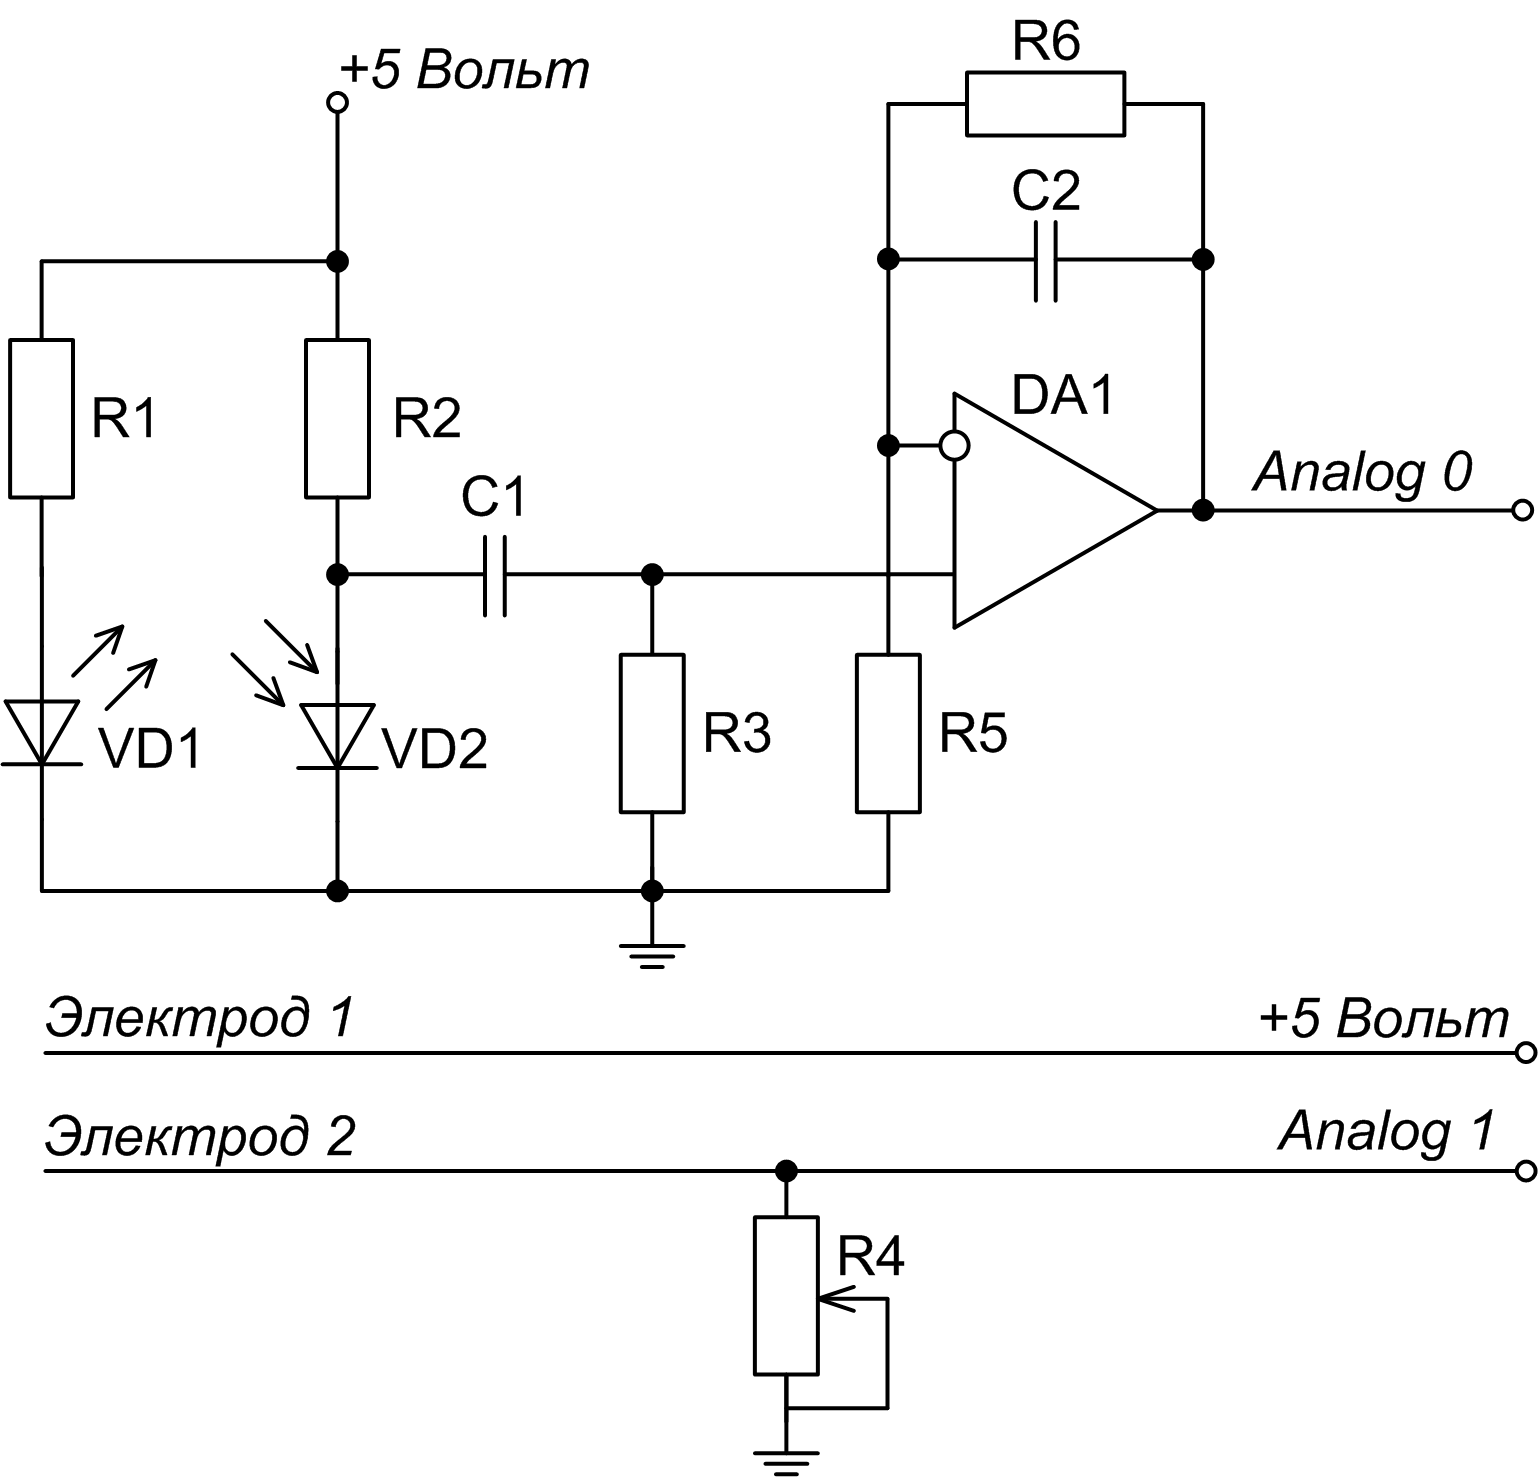
\includegraphics[scale=0.7]{18_2015_fig1}
  \caption{Измерительная подсистема} \label{latij1}
\end{figure}


\begin{figure}[h!]
  \centering 
  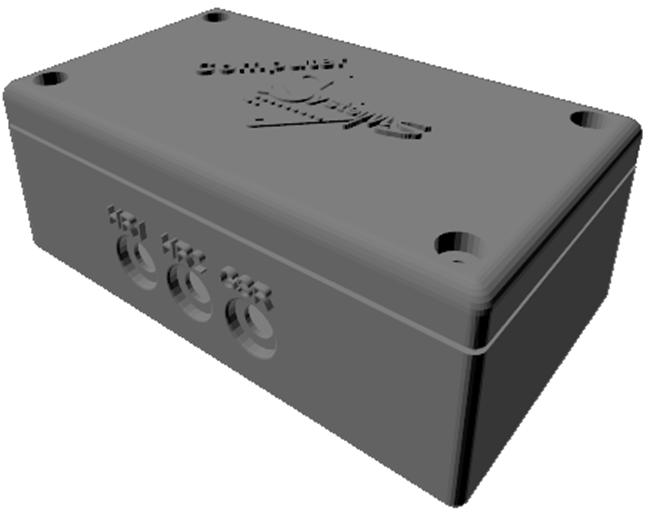
\includegraphics[scale=0.35]{18_2015_fig2} 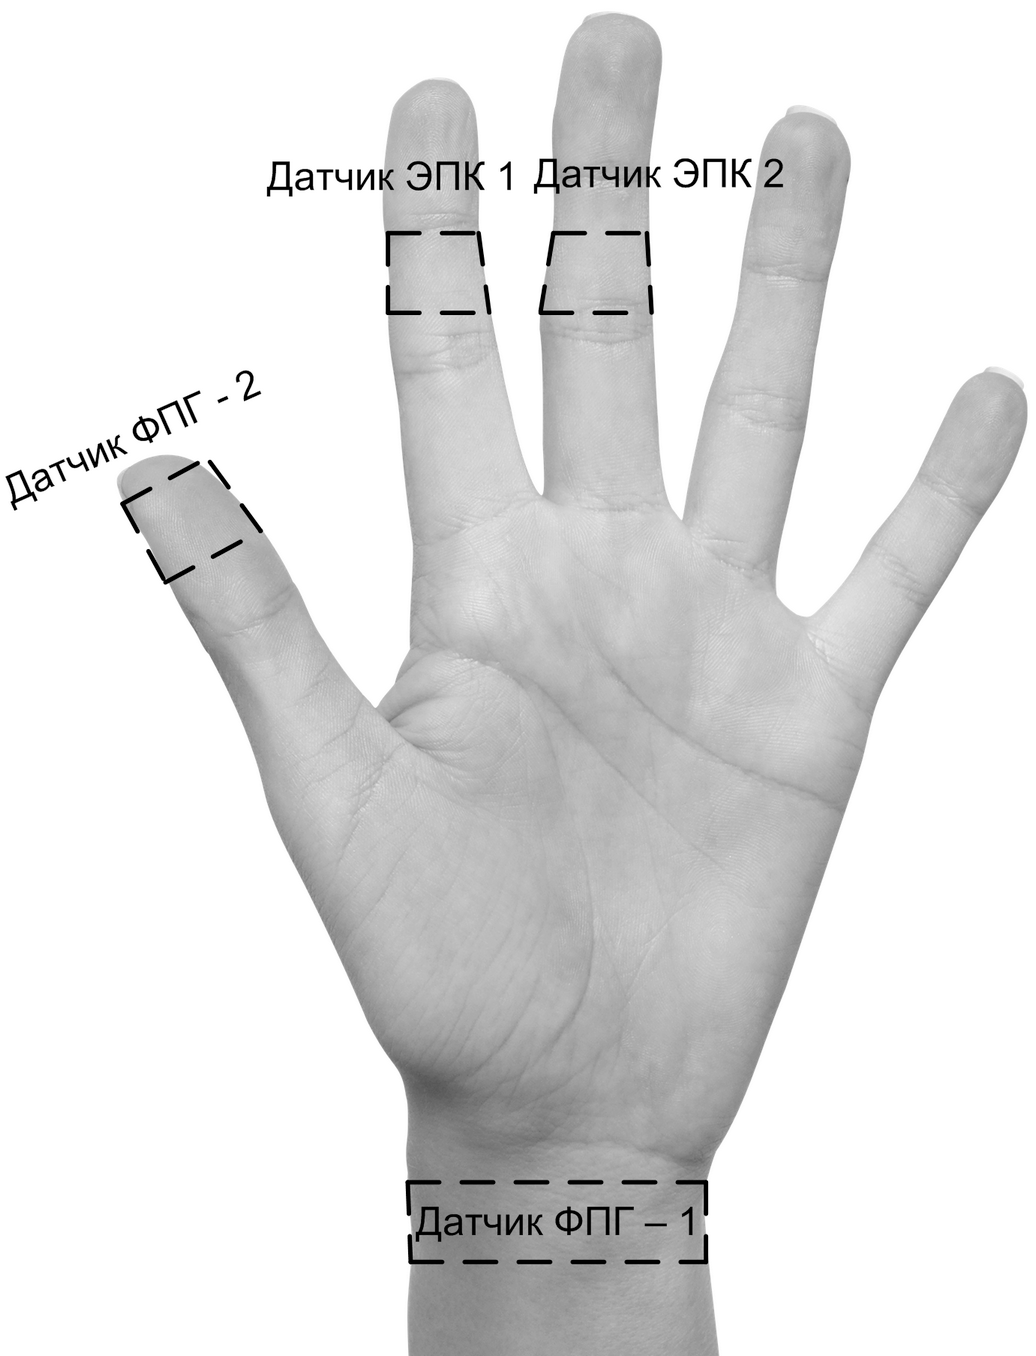
\includegraphics[scale=0.15]{18_2015_fig3} 
  \caption{3D-модель корпуса и схема крепления датчиков} \label{latij2}
\end{figure}

На рисунке \ref{latij2} можно видеть модель для изготовления корпуса устройства методом 3D-печати.

Для подключения щупов (одного для измерения ЭПК, и двух для ЧСС) применяется обычный аудио-разъем 3.5 мм TRS. Для крепления датчиков на текущий момент используются текстильные застёжки (места креплений можно видеть на рисунке \ref{latij2}).

%\begin{figure}[h!]
%  \centering 
%  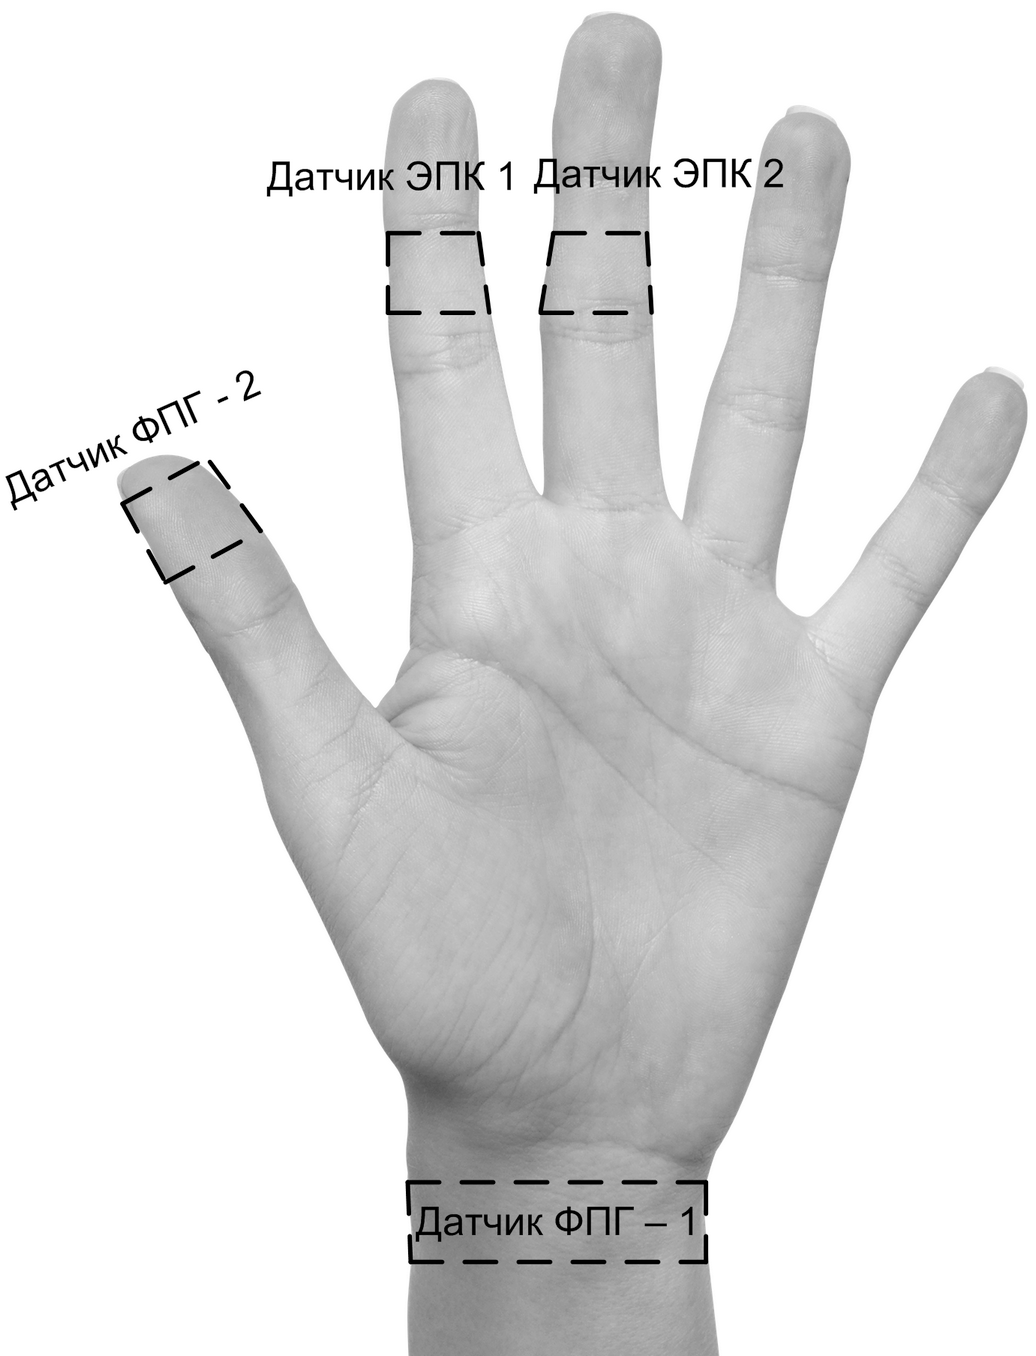
\includegraphics[scale=0.2]{18_2015_fig3} 
%  \caption{Схема крепления датчиков} \label{latij3}
%\end{figure}

Данные передаются в ПК по шине USB, которая одновременно осуществляет питание устройства. Таблица, формируемая принимающим данные ПО, сохраняется в формате CSV для последующего анализа (рисунки \ref{latij4} и \ref{latij5} демонстрируют иллюстративный экран отрисовки снимаемых кривых и фрагмент формируемой таблицы).


\begin{figure}[h!]
  \centering 
  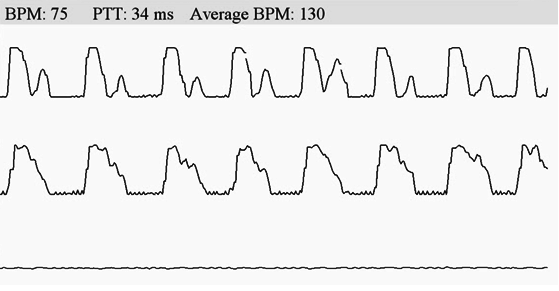
\includegraphics[scale=0.5]{18_2015_fig4}
  \caption{Первичная визуализация средствами processing} \label{latij4}
\end{figure}

\begin{figure}[h!]
  \centering 
  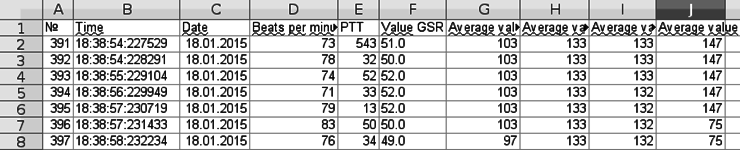
\includegraphics[scale=0.67]{18_2015_fig5}
  \caption{Фрагмент лог-файла} \label{latij5}
\end{figure}

\begin{thebibliography}{9}
\bibitem{bib1} {Kostiuk D.A., Derechennik S.S., Shitikov A.V., Latiy O.O. Approach to evaluate effectiveness of human-computer interaction with contemporary GUI // Третя мiжнародна науково-практична конференцiя FOSS Lviv 2013: Збiрник науковых праць, Львiв, 18–21 квiтня 2013 р. – Львiв, 2013. – С. 85–87.}
\bibitem{bib2} {Лацiй А.А., Касцюк Д.А. Апаратны модуль ацэнкi стану карыстальнiка ПК на базе Arduino // П'ята науково-практична конференцiя FOSS Lviv 2015: Збiрник наукових праць. Львiв, 23–26 квiтня 2015 р. – С. 64–66.}\end{thebibliography}
\end{document}

%%%\chapter{LVEE Winter 2014}
%\documentclass[10pt, a5paper]{article}
\usepackage{pdfpages}
\usepackage{parallel}
\usepackage[T2A]{fontenc}
\usepackage{ucs}
\usepackage[utf8x]{inputenc}
\usepackage[polish,english,russian]{babel}
\usepackage{hyperref}
\usepackage{rotating}
\usepackage[inner=2cm,top=1.8cm,outer=2cm,bottom=2.3cm,nohead]{geometry}
\usepackage{listings}
\usepackage{graphicx}
\usepackage{wrapfig}
\usepackage{longtable}
\usepackage{indentfirst}
\usepackage{array}
\newcolumntype{P}[1]{>{\raggedright\arraybackslash}p{#1}}
\frenchspacing
\usepackage{fixltx2e} %text sub- and superscripts
\usepackage{icomma} % коскі ў матэматычным рэжыме
\PreloadUnicodePage{4}

\newcommand{\longpage}{\enlargethispage{\baselineskip}}
\newcommand{\shortpage}{\enlargethispage{-\baselineskip}}

\def\switchlang#1{\expandafter\csname switchlang#1\endcsname}
\def\switchlangbe{
\let\saverefname=\refname%
\def\refname{Літаратура}%
\def\figurename{Іл.}%
}
\def\switchlangen{
\let\saverefname=\refname%
\def\refname{References}%
\def\figurename{Fig.}%
}
\def\switchlangru{
\let\saverefname=\refname%
\let\savefigurename=\figurename%
\def\refname{Литература}%
\def\figurename{Рис.}%
}

\hyphenation{admi-ni-stra-tive}
\hyphenation{ex-pe-ri-ence}
\hyphenation{fle-xi-bi-li-ty}
\hyphenation{Py-thon}
\hyphenation{ma-the-ma-ti-cal}
\hyphenation{re-ported}
\hyphenation{imp-le-menta-tions}
\hyphenation{pro-vides}
\hyphenation{en-gi-neering}
\hyphenation{com-pa-ti-bi-li-ty}
\hyphenation{im-pos-sible}
\hyphenation{desk-top}
\hyphenation{elec-tro-nic}
\hyphenation{com-pa-ny}
\hyphenation{de-ve-lop-ment}
\hyphenation{de-ve-loping}
\hyphenation{de-ve-lop}
\hyphenation{da-ta-ba-se}
\hyphenation{plat-forms}
\hyphenation{or-ga-ni-za-tion}
\hyphenation{pro-gramming}
\hyphenation{in-stru-ments}
\hyphenation{Li-nux}
\hyphenation{sour-ce}
\hyphenation{en-vi-ron-ment}
\hyphenation{Te-le-pathy}
\hyphenation{Li-nux-ov-ka}
\hyphenation{Open-BSD}
\hyphenation{Free-BSD}
\hyphenation{men-ti-on-ed}
\hyphenation{app-li-ca-tion}

\def\progref!#1!{\texttt{#1}}
\renewcommand{\arraystretch}{2} %Іначай формулы ў матрыцы зліпаюцца з лініямі
\usepackage{array}

\def\interview #1 (#2), #3, #4, #5\par{

\section[#1, #3, #4]{#1 -- #3, #4}
\def\qname{LVEE}
\def\aname{#1}
\def\q ##1\par{{\noindent \bf \qname: ##1 }\par}
\def\a{{\noindent \bf \aname: } \def\qname{L}\def\aname{#2}}
}

\def\interview* #1 (#2), #3, #4, #5\par{

\section*{#1\\{\small\rm #3, #4. #5}}

\def\qname{LVEE}
\def\aname{#1}
\def\q ##1\par{{\noindent \bf \qname: ##1 }\par}
\def\a{{\noindent \bf \aname: } \def\qname{L}\def\aname{#2}}
}

\switchlang{en}
\begin{document}
\title{Virtualization"=based illustrated reviews of the software history}
\author{Dmitriy Kostiuk, Pavel Lutsiuk, Sergey Vlasenko, \\ Vitaliy Zheludok "--- Brest, Belarus\footnote{\url{dmitriykostiuk@gmail.com}, \url{http://lvee.org/ru/abstracts/144}}}
\maketitle
\begin{abstract}
Experience of using virtual machines instead of screenshots in a visual timeline of GUI is reviewed. Availability of materials is considered as far as problems of QEMU"=based nested virtualiza\-tion. A solution is proposed for free distribution of F/LOSS virtualized items with a possibility to automatically integrate proprietary ones in case of their presence. 
\end{abstract}
Although technically working with the new information technologies doesn't demands knowing the history of their development, however specialist who formulates or applies modern theory without knowledge of its history, runs the risk of repeating the mistakes of predecessors personally one by one.

In the context of spoken above statement this project lies, providing the user of a local network or a standalone workstation with the set of chronologically HTML documents, each with a description of the specific graphical operating system and its live illustration in the form of built"=in frame with the screen of a running virtual machine (thanks to the performance of today's notebooks and desktop PCs, this task is easy enough). The information content of this project is based on the lecture course on the history of graphical user interface, including 40 desktop and 30 mobile operating systems and desktop environments.

Technical infrastructure implementing such informational materials, is close to one reviewed in \cite{kostiuk1} and includes following components: 
\begin{itemize}
\item QEMU virtual machine with hardware virtualization support,
\item noVNC VNC client, written in JavaScript and HTML5, 
\item JavaScript framework to display informational materials in one interactive timeline.
\end{itemize}

Running the scheme shown on the figure 1 is done by a startup script, which scans subdirectories in search for the information elements: pages with the content, virtual machine images and scripts to run them. Script passes VNC port numbers to discovered virtual machines and reconstructs HTML document to include of pages with information materials into timeline. This component based approach allows to divide the information, making free/libre parts publicly available on the net\-work, and taking away from public access those virtualized systems, which can not be redistributed due to the terms of commercial licenses.

\begin{figure}[h!]
  \centering
  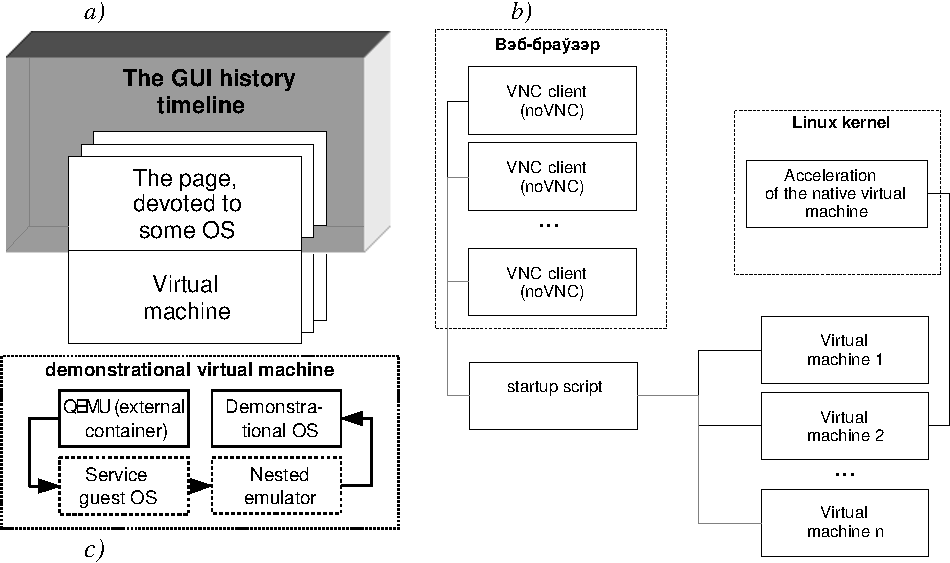
\includegraphics[scale=0.65]{100_2014_w-kostiuk1crop_en}
  \caption{Scheme of the document building (a), and components interaction (b) with nested virtualization (c)}
\end{figure}

The virtual machine is used as a fully isolated container storing a snapshot of the running OS \cite{kostiuk2}. Choice of QEMU is caused by the extremely simple transfer of virtual machine images between computers, and also by its ability to emulate not only x86"=compatible platforms, but also ones based on SPARC, PowerPC, Motorola 68k, MIPS and ARM processors, which are necessary to run many operating systems from 80s and 90s. However, currently multiplatformness of QEMU is poorly used, because the support of peripheral devices on alternative platforms at this emulator is rarely sufficient to boot ancient operating systems.

At the same time, there are emulators available to support virtually all ancient Intel"=incompatible systems "---community"=developed ones or created as the part of commercial SDK. The first variant is more common in desktop operating systems, so it was possible to enrich the timeline with Xerox Alto, Amiga, RiscOS, Apple Lisa, MacOS of 1.x, 7.x and X versions. Proprietary emulators for desktop operating systems are rare case and usually belong to the manufacturer of the OS, as in the case of Xerox GlobalView emulator. In case of mobile operating systems emulators from the SDK are dominating, such as Psion EPOC16 and EPOC32, PalmOS, Magic Cap, Windows CE, pre"=release versions of Android SDK. For now we use only one community"=developed mobile OS emulator "---Open Einstein project, which allows to run NewtonOS.

However, all these emulators don't support snapshots and the VNC protocol. Therefore a large part of demos is build along with the the nested virtualization scheme (see Fig. 1) where QEMU plays the role of an external container. 

Of course many operating systems do not require nested virtualiza\-tion and so internal emulator is not used for them. That's the case of desktop Windows OS oif 1.x, 2.x, 3.x and 95 versions, as far as IBM OS/2 2.x and 4.x, GEM from Digital Research, GEOS by Berkeley Softworks, as well as a number of mobile operating systems: Pen \linebreak Windows, Maemo, Android, WebOS (not least due to the fact that QEMU is often included in mobile SDK).

Freely distributable part of the timeline contains free/libre software systems (having such licenses from the very beginning, or opensourced because of the extreme aging or being a free clone of the abandoned commercial system). That's about different Unix"=based and Linux"=based desktop environments for desktop and mobile computers as well as GEM, Amiga, RiscOS, and HaikuOS.

The timeline material is still at the stage of filling; at this point the review has some missing objects, which have still played an important role in the history of graphical operating systems. Mainly these are new OS versions from Microsoft and Apple. In addition, DOS shell Visi On, and NeXTSTEP are incompatible with the current versions of QEMU. Currently we use Linux"=based GNUStep DE as the NeXTSTEP replacement. The problem with the Visi On can be solved using Bochs and VirtualBox, which is undesirable from the portability and resources consumption points of view.

The number of historically important GUI shells without runnable versions  appeared to be surprisingly small: currently this row includes multi"=window interface of Smalltalk from the late 70s, Xerox Star \linebreak Document Processor, as well as two mobile systems: PenPoint OS and IBM Simon. 

One more component can be seen in the scheme of embedded virtua\-lization "--- a service guest OS, which is used to start the nested emulator. Its choice is determined by the requirement of the minimum memory consumption, usage of idle CPU cycles, as well as support for USB bus emulation, which allows to emulate pointing devices in absolute coordinates. The latter requirement is important for a comfortable mouse control in a virtual machine \cite{kostiuk1}. As a service guest operating system in addition to multiple versions of Linux we have used FreeDOS and ReactOS. It should be further noted that ReactOS perfectly meets all three requirements, and thus in our own experience it is the first case of its successful application for some practical needs.


\begin{thebibliography}{9}
\bibitem{kostiuk1} Костюк Д.А. Особенности использования виртуализованных окружений, внедренных в презентационные материалы // Восьмая конференция «Cвободное программное обеспечение высшей школе»: тез. докл. / Переславль, 26--27 января 2012  года. М.: Альт Линукс, 2012. "---C. 83--86.
\bibitem{kostiuk2} Костюк Д.А., Дереченник С.С. Построение прозрачных виртуализованных окружений для изоляции уязвимых программных систем // Комплексная защита информации: матер. XVI научно-практич. конф., Гродно, 17--20 мая 2011 г. Гродно, 2011. "---С. 209--212. 
\end{thebibliography}
\end{document}

%\input{101_2014_w_LastName}
\documentclass[10pt, a5paper]{article}
\usepackage{pdfpages}
\usepackage{parallel}
\usepackage[T2A]{fontenc}
\usepackage{ucs}
\usepackage[utf8x]{inputenc}
\usepackage[polish,english,russian]{babel}
\usepackage{hyperref}
\usepackage{rotating}
\usepackage[inner=2cm,top=1.8cm,outer=2cm,bottom=2.3cm,nohead]{geometry}
\usepackage{listings}
\usepackage{graphicx}
\usepackage{wrapfig}
\usepackage{longtable}
\usepackage{indentfirst}
\usepackage{array}
\newcolumntype{P}[1]{>{\raggedright\arraybackslash}p{#1}}
\frenchspacing
\usepackage{fixltx2e} %text sub- and superscripts
\usepackage{icomma} % коскі ў матэматычным рэжыме
\PreloadUnicodePage{4}

\newcommand{\longpage}{\enlargethispage{\baselineskip}}
\newcommand{\shortpage}{\enlargethispage{-\baselineskip}}

\def\switchlang#1{\expandafter\csname switchlang#1\endcsname}
\def\switchlangbe{
\let\saverefname=\refname%
\def\refname{Літаратура}%
\def\figurename{Іл.}%
}
\def\switchlangen{
\let\saverefname=\refname%
\def\refname{References}%
\def\figurename{Fig.}%
}
\def\switchlangru{
\let\saverefname=\refname%
\let\savefigurename=\figurename%
\def\refname{Литература}%
\def\figurename{Рис.}%
}

\hyphenation{admi-ni-stra-tive}
\hyphenation{ex-pe-ri-ence}
\hyphenation{fle-xi-bi-li-ty}
\hyphenation{Py-thon}
\hyphenation{ma-the-ma-ti-cal}
\hyphenation{re-ported}
\hyphenation{imp-le-menta-tions}
\hyphenation{pro-vides}
\hyphenation{en-gi-neering}
\hyphenation{com-pa-ti-bi-li-ty}
\hyphenation{im-pos-sible}
\hyphenation{desk-top}
\hyphenation{elec-tro-nic}
\hyphenation{com-pa-ny}
\hyphenation{de-ve-lop-ment}
\hyphenation{de-ve-loping}
\hyphenation{de-ve-lop}
\hyphenation{da-ta-ba-se}
\hyphenation{plat-forms}
\hyphenation{or-ga-ni-za-tion}
\hyphenation{pro-gramming}
\hyphenation{in-stru-ments}
\hyphenation{Li-nux}
\hyphenation{sour-ce}
\hyphenation{en-vi-ron-ment}
\hyphenation{Te-le-pathy}
\hyphenation{Li-nux-ov-ka}
\hyphenation{Open-BSD}
\hyphenation{Free-BSD}
\hyphenation{men-ti-on-ed}
\hyphenation{app-li-ca-tion}

\def\progref!#1!{\texttt{#1}}
\renewcommand{\arraystretch}{2} %Іначай формулы ў матрыцы зліпаюцца з лініямі
\usepackage{array}

\def\interview #1 (#2), #3, #4, #5\par{

\section[#1, #3, #4]{#1 -- #3, #4}
\def\qname{LVEE}
\def\aname{#1}
\def\q ##1\par{{\noindent \bf \qname: ##1 }\par}
\def\a{{\noindent \bf \aname: } \def\qname{L}\def\aname{#2}}
}

\def\interview* #1 (#2), #3, #4, #5\par{

\section*{#1\\{\small\rm #3, #4. #5}}

\def\qname{LVEE}
\def\aname{#1}
\def\q ##1\par{{\noindent \bf \qname: ##1 }\par}
\def\a{{\noindent \bf \aname: } \def\qname{L}\def\aname{#2}}
}

%\frenchspacing
\begin{document}
\title{Голос спонсора: ITS Partner}
%\author{}
\date{}
\maketitle%

~

\end{document}



\documentclass[10pt, a5paper]{article}
\usepackage{pdfpages}
\usepackage{parallel}
\usepackage[T2A]{fontenc}
\usepackage{ucs}
\usepackage[utf8x]{inputenc}
\usepackage[polish,english,russian]{babel}
\usepackage{hyperref}
\usepackage{rotating}
\usepackage[inner=2cm,top=1.8cm,outer=2cm,bottom=2.3cm,nohead]{geometry}
\usepackage{listings}
\usepackage{graphicx}
\usepackage{wrapfig}
\usepackage{longtable}
\usepackage{indentfirst}
\usepackage{array}
\newcolumntype{P}[1]{>{\raggedright\arraybackslash}p{#1}}
\frenchspacing
\usepackage{fixltx2e} %text sub- and superscripts
\usepackage{icomma} % коскі ў матэматычным рэжыме
\PreloadUnicodePage{4}

\newcommand{\longpage}{\enlargethispage{\baselineskip}}
\newcommand{\shortpage}{\enlargethispage{-\baselineskip}}

\def\switchlang#1{\expandafter\csname switchlang#1\endcsname}
\def\switchlangbe{
\let\saverefname=\refname%
\def\refname{Літаратура}%
\def\figurename{Іл.}%
}
\def\switchlangen{
\let\saverefname=\refname%
\def\refname{References}%
\def\figurename{Fig.}%
}
\def\switchlangru{
\let\saverefname=\refname%
\let\savefigurename=\figurename%
\def\refname{Литература}%
\def\figurename{Рис.}%
}

\hyphenation{admi-ni-stra-tive}
\hyphenation{ex-pe-ri-ence}
\hyphenation{fle-xi-bi-li-ty}
\hyphenation{Py-thon}
\hyphenation{ma-the-ma-ti-cal}
\hyphenation{re-ported}
\hyphenation{imp-le-menta-tions}
\hyphenation{pro-vides}
\hyphenation{en-gi-neering}
\hyphenation{com-pa-ti-bi-li-ty}
\hyphenation{im-pos-sible}
\hyphenation{desk-top}
\hyphenation{elec-tro-nic}
\hyphenation{com-pa-ny}
\hyphenation{de-ve-lop-ment}
\hyphenation{de-ve-loping}
\hyphenation{de-ve-lop}
\hyphenation{da-ta-ba-se}
\hyphenation{plat-forms}
\hyphenation{or-ga-ni-za-tion}
\hyphenation{pro-gramming}
\hyphenation{in-stru-ments}
\hyphenation{Li-nux}
\hyphenation{sour-ce}
\hyphenation{en-vi-ron-ment}
\hyphenation{Te-le-pathy}
\hyphenation{Li-nux-ov-ka}
\hyphenation{Open-BSD}
\hyphenation{Free-BSD}
\hyphenation{men-ti-on-ed}
\hyphenation{app-li-ca-tion}

\def\progref!#1!{\texttt{#1}}
\renewcommand{\arraystretch}{2} %Іначай формулы ў матрыцы зліпаюцца з лініямі
\usepackage{array}

\def\interview #1 (#2), #3, #4, #5\par{

\section[#1, #3, #4]{#1 -- #3, #4}
\def\qname{LVEE}
\def\aname{#1}
\def\q ##1\par{{\noindent \bf \qname: ##1 }\par}
\def\a{{\noindent \bf \aname: } \def\qname{L}\def\aname{#2}}
}

\def\interview* #1 (#2), #3, #4, #5\par{

\section*{#1\\{\small\rm #3, #4. #5}}

\def\qname{LVEE}
\def\aname{#1}
\def\q ##1\par{{\noindent \bf \qname: ##1 }\par}
\def\a{{\noindent \bf \aname: } \def\qname{L}\def\aname{#2}}
}

\begin{document}
\title{Голос спонсора: SaM Solutions}
%\author{}
\date{}
\maketitle

Компания SaM Solutions выступает в роли системо-образующего спонсора конференции Linux Vacation Eastern Europe с момента рождения LVEE в 2005 году и на протяжении всех лет её проведения. 

Сложившаяся корпоративная практика не случайна. Продукты и решения, задействующие Linux и другие Free/Open Source Software проекты, составляют заметную часть пакета разработок SaM Solutions. Кадровая политика компании направлена на поощрение профессионального развития своих сотрудников, организацию их эффективного отдыха и привлечение хорошо мотивированных кандидатов к работе на компанию. Формат конференции LVEE успешно позволяет решать все три задачи. 

Одним из подразделений компании является отдел Linux и \linebreak Embbeded. Специалисты компании на протяжении десятилетий работают с СПО. Компанией реализован ряд проектов по адаптации ОС GNU/Linux для работы в различных устройствах, построенных на таких платформах как ARM, PowerPC, x86, MIPS. В последние годы "--- на ведущие позиции выходит разработка управляющего ПО для серверов Enterprise-класса, от низкоуровнего BMC Firmware на основе Linux до высокоуровневых систем контроля виртуализации и графических интерфейсов управления, от прошивок устройств хранения данных до BSP интегрированных плат для разработчика. Надёжность, качество и широкая функциональность множества свободных проектов позволяет строить нам системы любого уровня и сложности, опираясь на высококачественные готовые компоненты.

В рамках направления Linux и Embedded успешно выполнены проекты для таких знаковых заказчиков, как  Novell/SUSE, Fujitsu Technology Solutions  и осуществляется партнёрство с компаниями IBM и Oracle/Sun в области Open Source решений.

Мы разрабатываем, модифицируем и адаптируем различное свободное программное обеспечение для наших заказчиков, но не забываем и о своих нуждах "--- наши сотрудники используют в своей работе существующие програмные продукты и вносят вклад в их развитие. Часть внутренней инфраструктуры, а именно интранет-сеть компании, тестовые стенды отдела контроля качества, рабочие места сотрудников профильных подразделений "--- также работает под управлением СПО (серверные и десктопные платформы GNU/Linux и FreeBSD). 

В минувшем году, в рамках реорганизации, был разработан долгосрочный план развития направления Linux и Embedded в SaM Solutions. В нём впервые были кодифицированы уже имеющиеся внутренние неофициальные практики по взаимодействию с commu"=nity-based проектами. В частности разработаны меры и правила по
\begin{itemize}
  \item возврата изменений в родительские проекты (upstreaming);
  \item вхождения в состав постоянных разработчиков активно используемых нами FOSS-компонентов;
  \item публикации сообщений об ошибках (bug reporting);
  \item участия и помощи в организации community events;
  \item стимуляции докладов и участия в технических конференциях.
\end{itemize}
И план немедленно начал претворяться в жизнь.

Силами отдела организовано внутреннее обучение сотрудников на регулярной
основе. Был прочтен и опубликован курс по TDD. По согласованию с автором
опубликован курс Debian/Ubuntu Packaging (видео, презентация и исходные
тексты презентации в \LaTeX).  Были организованы и проведены курсы по
обучению QA специалистов для направления Embeded Linux. Проведено
практическое занятие по основам виртуализации и эмуляции, организована
лекция по вопросу профилирования и оптимизации Ruby-кода, лекция о
High-availability кластерах и направлении развития технологии. Кроме того,
проводился семинар по Video4Linux2. Для создания и обучения кадрового
резерва на ближайшее будущее запланированы постоянно действующие внутренние
проекты в области Embedded Linux, результаты которых также запланированы к
публикации.

Визиты представительных делегаций на Embedded World 2012 и Linux Con Europe/Embedded LinuxCon Europe 2011 обогатили нас новыми идеями, куда можно
двигаться дальше и что сейчас актуально. А выступления на Software
Engineering Forum for Students, круглом столе по СПО в рамках TIBO-2012
и LVEE Winter 2012 позволили поделиться опытом с
заинтересованными сторонами.

В апреле состоялась Ганноверская промышленная ярмарка \linebreak (Hannover Messe
2013). Компания SaM Solutions была представлена отдельным стендом, на
котором демонстрировались наработки в области встроенного и системного ПО
на базе OS Linux. Идея «умного» дома вызвала неподдельный интерес у
посетителей стенда.

При поддержке SaM Solutions, с декабря 2011 года возобновились регулярные встречи Minsk Linux Users Groups, под названием <<Линуксовка в SaM Solutions>>. Техническое оснащение линуксовок и открытый формат встреч позволил им практически мгновенно стать заметным дискуссионным клубом по широкому спектру вопросов, прямо или косвенно связанных с СПО. Свободная картография (OpenStreetMap), технологии виртуализации, минский \linebreak hackerspace, Linux Mobile, бойкот Голливудской продукции, systemd, загрузчик u-boot, белорусская локализация GNOME --- это только часть тем, поднятых за последние линуксовки.

Быстрые и положительные изменения, как внутри компании SaM Solutions, так и в экосфере СПО (и Linux в частности) наполняют нас уверенностью, что направление движения выбрано верно.

\begin{figure}[h!]
\centering
\includegraphics[height=11.8cm]{48_spons_sams.pdf}
\end{figure}
\end{document}



\documentclass[10pt, a5paper]{article}
\usepackage{pdfpages}
\usepackage{parallel}
\usepackage[T2A]{fontenc}
\usepackage{ucs}
\usepackage[utf8x]{inputenc}
\usepackage[polish,english,russian]{babel}
\usepackage{hyperref}
\usepackage{rotating}
\usepackage[inner=2cm,top=1.8cm,outer=2cm,bottom=2.3cm,nohead]{geometry}
\usepackage{listings}
\usepackage{graphicx}
\usepackage{wrapfig}
\usepackage{longtable}
\usepackage{indentfirst}
\usepackage{array}
\newcolumntype{P}[1]{>{\raggedright\arraybackslash}p{#1}}
\frenchspacing
\usepackage{fixltx2e} %text sub- and superscripts
\usepackage{icomma} % коскі ў матэматычным рэжыме
\PreloadUnicodePage{4}

\newcommand{\longpage}{\enlargethispage{\baselineskip}}
\newcommand{\shortpage}{\enlargethispage{-\baselineskip}}

\def\switchlang#1{\expandafter\csname switchlang#1\endcsname}
\def\switchlangbe{
\let\saverefname=\refname%
\def\refname{Літаратура}%
\def\figurename{Іл.}%
}
\def\switchlangen{
\let\saverefname=\refname%
\def\refname{References}%
\def\figurename{Fig.}%
}
\def\switchlangru{
\let\saverefname=\refname%
\let\savefigurename=\figurename%
\def\refname{Литература}%
\def\figurename{Рис.}%
}

\hyphenation{admi-ni-stra-tive}
\hyphenation{ex-pe-ri-ence}
\hyphenation{fle-xi-bi-li-ty}
\hyphenation{Py-thon}
\hyphenation{ma-the-ma-ti-cal}
\hyphenation{re-ported}
\hyphenation{imp-le-menta-tions}
\hyphenation{pro-vides}
\hyphenation{en-gi-neering}
\hyphenation{com-pa-ti-bi-li-ty}
\hyphenation{im-pos-sible}
\hyphenation{desk-top}
\hyphenation{elec-tro-nic}
\hyphenation{com-pa-ny}
\hyphenation{de-ve-lop-ment}
\hyphenation{de-ve-loping}
\hyphenation{de-ve-lop}
\hyphenation{da-ta-ba-se}
\hyphenation{plat-forms}
\hyphenation{or-ga-ni-za-tion}
\hyphenation{pro-gramming}
\hyphenation{in-stru-ments}
\hyphenation{Li-nux}
\hyphenation{sour-ce}
\hyphenation{en-vi-ron-ment}
\hyphenation{Te-le-pathy}
\hyphenation{Li-nux-ov-ka}
\hyphenation{Open-BSD}
\hyphenation{Free-BSD}
\hyphenation{men-ti-on-ed}
\hyphenation{app-li-ca-tion}

\def\progref!#1!{\texttt{#1}}
\renewcommand{\arraystretch}{2} %Іначай формулы ў матрыцы зліпаюцца з лініямі
\usepackage{array}

\def\interview #1 (#2), #3, #4, #5\par{

\section[#1, #3, #4]{#1 -- #3, #4}
\def\qname{LVEE}
\def\aname{#1}
\def\q ##1\par{{\noindent \bf \qname: ##1 }\par}
\def\a{{\noindent \bf \aname: } \def\qname{L}\def\aname{#2}}
}

\def\interview* #1 (#2), #3, #4, #5\par{

\section*{#1\\{\small\rm #3, #4. #5}}

\def\qname{LVEE}
\def\aname{#1}
\def\q ##1\par{{\noindent \bf \qname: ##1 }\par}
\def\a{{\noindent \bf \aname: } \def\qname{L}\def\aname{#2}}
}

\begin{document}
\title{Голос спонсора: Conjur. Authorization in the cloud}
%\author{}
\date{}
\maketitle

\begin{figure}[h!]
\centering
\includegraphics{74_conjur-logo-1.pdf}
\end{figure}

Conjur is a cloud-native platform for directory services, authoriza\-tion, and audit for development and operations teams and their entire infrastructure. 

With 100\% API coverage and a scalable, easily deployable, high-availability architecture, Conjur reduces the time, cost, and complexity associated with building authorization management via complex home\-grown scripts and configuration management tools. Sometimes referred to as “Active Directory for the cloud”, Conjur runs in either a virtual machine or container, and works alongside a wide range identity and access management (IAM) solutions to solve access and authorization challenges: machine-to-machine permissions, deployment and access \linebreak rights to 
sensitive systems, and the auditing required to meet complian\-ce requirements. 

“Conjur is more than just an outstanding platform for managing authorization as a service: they are a partner that we can innovate with, and an essential part of achieving our vision and solving the hard problems that arise as we move our infrastructure into the cloud technologies that will drive our business forward.” 
- Mike Kail, VP of Operations, Netflix 

\section*{Why Conjur? }
Built with system administrators, DevOps professionals, and cloud architects in mind, Conjur natively supports a wide range of potential use cases. Some of the most common reasons why organizations select Conjur over building in-house solutions include: 
\begin{itemize}
\item {\bf Compliance}: auditable enforcement of both organizational and regulatory policies and rules, via existing reporting systems (e.g., SIEM platforms, SumoLogic, Splunk) 
\item {\bf Risk Management}: reduction of the attack surface for sensitive data
(credentials, SSL/SSH keys and certificates, secrets, etc.) by means of
Conjur’s policy and governance platform

\item {\bf DevOps Optimization}: integration of security \& controls in upstream development and operations work, ensuring consistency across all production systems. 
\item {\bf Access Intelligence}: unified control of identity (human \& machi\-ne) and permissions across entire infrastructure (bare metal, pri\-vate, public, cloud) helps prevent failures, without relying on legacy systems for policy governance and enforcement 
\end{itemize}

\section*{What is Conjur?}


Conjur is designed with two primary goals: (1) to provide an easy-to-use, well documented, extensible authorization system, and (2) to allow for non-disruptive integration into organizati\-onal workflows. 

This approach has resulted in a series of implementation benefits: 
\begin{itemize}
\item {\bf Ease of Integration}: Conjur is built with a DevOps optimized UX (CLI-driven), with 100\% API access from a variety of langua\-ges, and can be deployed as a Linux virtual appliance, or into bare-metal systems 
\item {\bf No Vendor Lock-In}: Conjur has been used in conjunction with all leading configuration management and DevOps tools (Puppet, Chef, Salt, Docker, etc.) 
\item {\bf HA Design}: Conjur’s system has been designed with high availa\-bility and fault tolerance, with a distributed configuration archi\-tecture and full fail-over/redundancy capabilities 
\item {\bf Minimal Dependencies}: Conjur is self-contained, requiring no external database or server  
\item {\bf Secure}: All communication is fully encrypted, following industry best practices for managing data in use and at rest; additionally, Conjur has invested in a rigorous third-party security analysis (results expected to be published Q4 FY14)
\end{itemize}

Learn more at \url{http://conjur.net}

\end{document}



\documentclass[10pt, a5paper]{article}
\usepackage{pdfpages}
\usepackage{parallel}
\usepackage[T2A]{fontenc}
\usepackage{ucs}
\usepackage[utf8x]{inputenc}
\usepackage[polish,english,russian]{babel}
\usepackage{hyperref}
\usepackage{rotating}
\usepackage[inner=2cm,top=1.8cm,outer=2cm,bottom=2.3cm,nohead]{geometry}
\usepackage{listings}
\usepackage{graphicx}
\usepackage{wrapfig}
\usepackage{longtable}
\usepackage{indentfirst}
\usepackage{array}
\newcolumntype{P}[1]{>{\raggedright\arraybackslash}p{#1}}
\frenchspacing
\usepackage{fixltx2e} %text sub- and superscripts
\usepackage{icomma} % коскі ў матэматычным рэжыме
\PreloadUnicodePage{4}

\newcommand{\longpage}{\enlargethispage{\baselineskip}}
\newcommand{\shortpage}{\enlargethispage{-\baselineskip}}

\def\switchlang#1{\expandafter\csname switchlang#1\endcsname}
\def\switchlangbe{
\let\saverefname=\refname%
\def\refname{Літаратура}%
\def\figurename{Іл.}%
}
\def\switchlangen{
\let\saverefname=\refname%
\def\refname{References}%
\def\figurename{Fig.}%
}
\def\switchlangru{
\let\saverefname=\refname%
\let\savefigurename=\figurename%
\def\refname{Литература}%
\def\figurename{Рис.}%
}

\hyphenation{admi-ni-stra-tive}
\hyphenation{ex-pe-ri-ence}
\hyphenation{fle-xi-bi-li-ty}
\hyphenation{Py-thon}
\hyphenation{ma-the-ma-ti-cal}
\hyphenation{re-ported}
\hyphenation{imp-le-menta-tions}
\hyphenation{pro-vides}
\hyphenation{en-gi-neering}
\hyphenation{com-pa-ti-bi-li-ty}
\hyphenation{im-pos-sible}
\hyphenation{desk-top}
\hyphenation{elec-tro-nic}
\hyphenation{com-pa-ny}
\hyphenation{de-ve-lop-ment}
\hyphenation{de-ve-loping}
\hyphenation{de-ve-lop}
\hyphenation{da-ta-ba-se}
\hyphenation{plat-forms}
\hyphenation{or-ga-ni-za-tion}
\hyphenation{pro-gramming}
\hyphenation{in-stru-ments}
\hyphenation{Li-nux}
\hyphenation{sour-ce}
\hyphenation{en-vi-ron-ment}
\hyphenation{Te-le-pathy}
\hyphenation{Li-nux-ov-ka}
\hyphenation{Open-BSD}
\hyphenation{Free-BSD}
\hyphenation{men-ti-on-ed}
\hyphenation{app-li-ca-tion}

\def\progref!#1!{\texttt{#1}}
\renewcommand{\arraystretch}{2} %Іначай формулы ў матрыцы зліпаюцца з лініямі
\usepackage{array}

\def\interview #1 (#2), #3, #4, #5\par{

\section[#1, #3, #4]{#1 -- #3, #4}
\def\qname{LVEE}
\def\aname{#1}
\def\q ##1\par{{\noindent \bf \qname: ##1 }\par}
\def\a{{\noindent \bf \aname: } \def\qname{L}\def\aname{#2}}
}

\def\interview* #1 (#2), #3, #4, #5\par{

\section*{#1\\{\small\rm #3, #4. #5}}

\def\qname{LVEE}
\def\aname{#1}
\def\q ##1\par{{\noindent \bf \qname: ##1 }\par}
\def\a{{\noindent \bf \aname: } \def\qname{L}\def\aname{#2}}
}

\begin{document}
\title{Голос спонсора: World of Tanks team}
%\author{}
\date{}
\maketitle

\subsection*{О проекте}

World of Tanks (Мир танков) "--- первый ММО проект ААА класса, созданный
белоруской командой. Разработчиками игра позиционируется как MMO"=экшн с
элементами ролевой игры, шутера и стратегии. Концепция <<World of Tanks>>
базируется на массовых командных танковых сражениях в режиме PvP. Онлайн
релиз русской версии игры состоялся 12 августа 2010 года, в марте 2011 года
состоялся <<китайский>> релиз, а в апреле 2011 года проект успешно вышел на
территории США и Европы.

Успех проекта World of Tanks можно оценить по целому ряду показателей:
количество активных игроков более 2 миллионов, рекордная цифра одновременной
игры "--- более 150.000 игроков на российском игровом кластере! В книгу
рекордов Гиннеса мы вошли 23 января 2011 года с показателем 91 311 игроков
он"=лайн. 

Дважды подряд в 2010 и 2011 году на Конференции Разработчиков Компьютерных
Игр (Москва) наш проект был признан Лучшей клиентской он"=лайн игрой (КРИ
2010) и Лучшей игрой (КРИ 2011).

В 2010 году по результатам международной выставки E3 (Лос"=Анжелес)
крупнейший ММО"=портал Massivly назвал наш проект New Concept 2010. В
настоящий момент определяются победители E3 2011. Мы сможем рассказать о
наших успехах уже при личной встрече на конференции LVEE 2011.

\subsection*{Подробности о проекте}

Игровые кластеры проекта находятся в дата"=центрах России, Германии, США и
Китая. Общее количество серверов в настоящий момент порядка 500, к концу
года мы планируем удвоить их количество.

Как игровые, так и прочие инфраструктурные сервера функционируют на базе
операционной системы CentOS.

Осенью 2010 года пики онлайна на российском игровом кластере достигали 30
тыс. В настоящий момент за счет высокотехнологичных решений наших
специалистов (включающих в себя оптимизацию сетевой инфраструктуры,
оптимизацию работы с базами данных, оптимизацию нашего серверного ПО) пик
он-лайна вырос до 150 тыс.

Высокая производительность достигается в т.~ч. за счет использования
free and open source software  как технологической основы для работы
серверной части самой масштабной ММО"=игры, а именно: CentOS,
MySQL, nginx, zabbix, nagios, cacti, python, django и т.~д.

\subsection*{О нас}

Над созданием проекта работает СООО <<Гейм Стрим>> "--- основной центр разработки
компании \url{Wargaming.net}. История компании "--- это 12"=летний опыт создания игр,
более 15 выпущенных проектов, среди которых <<Операция Багратион>>, а так же
<<Order of War>>, изданная Square Enix. В 2007 году мы объединились с минской
студией Arise. В 2010 из разработчика превратились в издателя "--- мы сами
осуществляем оперирование проекта World of Tanks. 

Наши награды на Конференции Разработчиков Компьютерных Игр (Москва): лучшая стратегическая игра КРИ"=2008 (проект <<Операция Багратион>>),
приз от прессы КРИ"=2009, лучшая компания"=разработчик КРИ"=2009 и КРИ"=2010, приз от индустрии КРИ 2011, приз зрительских симпатий КРИ 2011.

Сейчас в студии работает более 200 человек. Мы готовимся к запуску в
производство новых проектов и будем рады знакомству с талантливыми
специалистами. 

Нашим будущим сотрудникам мы предлагаем уникальную возможность работать над
онлайн"=проектами ААА класса, с применением передовых технологических
решений; реализовать себя, работая над сложными задачами; учиться у ведущих
специалистов отрасли. Со своей стороны мы создаём для этого все условия:
комфортный офис, современное техническое обеспечение рабочих мест, все
социальные гарантии, высокие белые зарплаты, обучение и т.~д. А ещё у нас
работают замечательные люди.

Наш контактный e-mail:  \url{rabota@wargaming.net}
Присоединяйтесь к команде World of Tanks!

\end{document}



\documentclass[10pt, a5paper]{article}
\usepackage{pdfpages}
\usepackage{parallel}
\usepackage[T2A]{fontenc}
\usepackage{ucs}
\usepackage[utf8x]{inputenc}
\usepackage[polish,english,russian]{babel}
\usepackage{hyperref}
\usepackage{rotating}
\usepackage[inner=2cm,top=1.8cm,outer=2cm,bottom=2.3cm,nohead]{geometry}
\usepackage{listings}
\usepackage{graphicx}
\usepackage{wrapfig}
\usepackage{longtable}
\usepackage{indentfirst}
\usepackage{array}
\newcolumntype{P}[1]{>{\raggedright\arraybackslash}p{#1}}
\frenchspacing
\usepackage{fixltx2e} %text sub- and superscripts
\usepackage{icomma} % коскі ў матэматычным рэжыме
\PreloadUnicodePage{4}

\newcommand{\longpage}{\enlargethispage{\baselineskip}}
\newcommand{\shortpage}{\enlargethispage{-\baselineskip}}

\def\switchlang#1{\expandafter\csname switchlang#1\endcsname}
\def\switchlangbe{
\let\saverefname=\refname%
\def\refname{Літаратура}%
\def\figurename{Іл.}%
}
\def\switchlangen{
\let\saverefname=\refname%
\def\refname{References}%
\def\figurename{Fig.}%
}
\def\switchlangru{
\let\saverefname=\refname%
\let\savefigurename=\figurename%
\def\refname{Литература}%
\def\figurename{Рис.}%
}

\hyphenation{admi-ni-stra-tive}
\hyphenation{ex-pe-ri-ence}
\hyphenation{fle-xi-bi-li-ty}
\hyphenation{Py-thon}
\hyphenation{ma-the-ma-ti-cal}
\hyphenation{re-ported}
\hyphenation{imp-le-menta-tions}
\hyphenation{pro-vides}
\hyphenation{en-gi-neering}
\hyphenation{com-pa-ti-bi-li-ty}
\hyphenation{im-pos-sible}
\hyphenation{desk-top}
\hyphenation{elec-tro-nic}
\hyphenation{com-pa-ny}
\hyphenation{de-ve-lop-ment}
\hyphenation{de-ve-loping}
\hyphenation{de-ve-lop}
\hyphenation{da-ta-ba-se}
\hyphenation{plat-forms}
\hyphenation{or-ga-ni-za-tion}
\hyphenation{pro-gramming}
\hyphenation{in-stru-ments}
\hyphenation{Li-nux}
\hyphenation{sour-ce}
\hyphenation{en-vi-ron-ment}
\hyphenation{Te-le-pathy}
\hyphenation{Li-nux-ov-ka}
\hyphenation{Open-BSD}
\hyphenation{Free-BSD}
\hyphenation{men-ti-on-ed}
\hyphenation{app-li-ca-tion}

\def\progref!#1!{\texttt{#1}}
\renewcommand{\arraystretch}{2} %Іначай формулы ў матрыцы зліпаюцца з лініямі
\usepackage{array}

\def\interview #1 (#2), #3, #4, #5\par{

\section[#1, #3, #4]{#1 -- #3, #4}
\def\qname{LVEE}
\def\aname{#1}
\def\q ##1\par{{\noindent \bf \qname: ##1 }\par}
\def\a{{\noindent \bf \aname: } \def\qname{L}\def\aname{#2}}
}

\def\interview* #1 (#2), #3, #4, #5\par{

\section*{#1\\{\small\rm #3, #4. #5}}

\def\qname{LVEE}
\def\aname{#1}
\def\q ##1\par{{\noindent \bf \qname: ##1 }\par}
\def\a{{\noindent \bf \aname: } \def\qname{L}\def\aname{#2}}
}

\begin{document}
\title{Голос спонсора: EPAM Systems}
%\author{}
\date{}
\maketitle

Компания EPAM Systems не первый год является спонсором международной конференции разработчиков и пользователей свободного программного обеспечения LVEE (Linux Vacation / Eastern Europe). Этот год также не стал исключением. Пожалуй, LVEE является самым значимым событием для русскоязычных разработчиков и тестировщиков Open Source. Каждое лето здесь встречаются начинающие специалисты и «ветераны»"=разработчики из десятка стран для обмена опытом и общения на профессиональные темы. Наши специалисты также активно участвуют в данной конференции: в качестве докладчиков и организаторов/волонтёров. Это уникальная в своём роде конференция, и именно поэтому EPAM Systems очередной раз принимает участие в LVEE в качестве спонсора.


EPAM Systems "--- одна из крупнейших компаний"=поставщиков\linebreak услуг в области разработки программного обеспечения и решений на территории СНГ и Центральной и Восточной Европы. Созданная в 1993 году, сегодня она имеет представительства в 12 странах мира, в штате работают более 9 тыс. сотрудников, из которых более 3 тыс. "--- в Беларуси. Рост компании обеспечивается за счет собственных обучающих программ и передаче опыта от больших специалистов до начинающих разработчиков. Компания EPAM Systems выполняет проекты более чем в 30 странах мира. Основные направления деятельности: разработка, тестирование, сопровождение и поддержка заказного программного обеспечения и бизнес"=приложений, а также ИТ"=консалтинг с учетом отраслевой специфики бизнеса.

Наша компания участвует в проектах с такими крупными, хорошо известными заказчиками как Google, Novell, Infoblox, Parallels, 10Gen и др., так и с небольшими, в том числе и с начинающими свой путь в софтверном бизнесе.


К примеру, для Infoblox была реализована связка между WebUI с BIND и DHCP. Для этого был разработан комплекс решений под управлением Shell и Python скриптов, а также механизм позволяющий вносить правки в BIND и DHCP на языке C. Также был разработан развернутый функционал, автоматизирующий инсталляцию новых устройств и их эксплуатацию, что позволяет значительно упростить управление данными. Встроенный Web"=интерфейс позволяет разворачивать, управлять сервисами DNS, DNSSEC, DHCP, IPAM, устанавливать новые версии ПО, архивировать и восстанавливать из архивов необходимые данные, восстанавливать их после аварии, проводить мониторинг сети и создавать отчеты без необходимости обращения к командной строке.


Еще одним решением, реализованным для компании Infoblox, являлся программный продукт, позволяющий контролировать сетевые изменения, таким образом, облегчая идентификацию трудноуловимых проблем конфигурации и соответствие требованиям. Вместо того чтобы просто регистрировать изменения, система использует внесенную информацию для проверки, анализа и автоматической обработки сетевых изменений. Благодаря инновационной, квалифицированной, глубокой технике логического анализа, программа изолирует проблемы исправности и конфигурации до того, как они могут вызвать более серьезные сбои.


Разработанная для анализа сложных сетей система изучает сеть, собирает ключевую информацию, применяет встроенную технику логического анализа и создает оценку исправности сети и список проблем, требующих принятие мер для улучшения качества работы сети.


Правильное использование свободного ПО в разработках сокращает и расходы на покупку лицензионных программ, и трудозатраты при создании коммерческого ПО. Немалую роль для достижения превосходного результата играет привлечение к разработке опытных специалистов. LVEE способствует появлению таких специалистов, развитию их навыков и расширению кругозора. Хотелось бы пожелать участникам конференции интересных проектов и максимум пользы от участия в LVEE.


\end{document}



\documentclass[10pt, a5paper]{article}
\usepackage{ucs}
\usepackage[utf8]{inputenc}
\usepackage[T2A]{fontenc}
\usepackage[english, russian]{babel}
\usepackage{hyperref}
\usepackage{geometry}
\usepackage{graphicx}
\frenchspacing
\begin{document}
\title{Голос спонсора: Ciklum}
%\author{}
\date{}
\maketitle
\begin{figure}[ht]
\centering{\includegraphics[width=12cm]{51_spons_ciklum1}}
%\label{pic:fl1}
%\caption{Схема инфракрасного приемника}
\end{figure}

Ciklum is a Danish innovative IT outsourcing company specializing in nearshore software development. 
Established in 2002, Ciklum employs more than 1200+ IT specialists worldwide with more than 130+ current clients own development teams. Ciklum has pioneered a unique business model in Ukraine where employees have direct communication with the client and are equal to clients` home-based colleagues. In Ciklum we are working on the development of different kind of projects: from cross-platform end-user applications to multifunctional B2B scalable solutions.

What Ciklum offers to developers?
\begin{itemize}
\item Variety of knowledge sharing and training opportunities within Ciklum Knowledge Exchange community
\item A lot of various technical seminars
\item Unique working environment where you communicate and work directly with international businesses
\item Possibility to work in a big and successful company
\item Competitive salary
\item Career and professional growth 
\item Long-term employment with 20 working-days paid vacation and other social benefits 
\item State of the art, cool, centrally located offices with warm atmosphere which creates really good working conditions
\end{itemize}

Ciklum has four development offices in the four largest cities in Ukraine \& Belarus (Kyiv, Minsk, Kharkiv, Dnipropetrovsk, Donetsk) and two development offices in Pakistan (Lahore, Islamabad), as well as representative offices in Denmark, Sweden, United Kingdom, Switzerland, Germany and the Netherlands. 

Join Ciklum and «Cross the Borders» together with us!

\begin{figure}[hb]
\centering{\includegraphics[width=12cm]{51_spons_ciklum2}}
%\label{pic:fl1}
%\caption{Схема инфракрасного приемника}
\end{figure}

\end{document}



\documentclass[10pt, a5paper]{article}
\usepackage{pdfpages}
\usepackage{parallel}
\usepackage[T2A]{fontenc}
\usepackage{ucs}
\usepackage[utf8x]{inputenc}
\usepackage[polish,english,russian]{babel}
\usepackage{hyperref}
\usepackage{rotating}
\usepackage[inner=2cm,top=1.8cm,outer=2cm,bottom=2.3cm,nohead]{geometry}
\usepackage{listings}
\usepackage{graphicx}
\usepackage{wrapfig}
\usepackage{longtable}
\usepackage{indentfirst}
\usepackage{array}
\newcolumntype{P}[1]{>{\raggedright\arraybackslash}p{#1}}
\frenchspacing
\usepackage{fixltx2e} %text sub- and superscripts
\usepackage{icomma} % коскі ў матэматычным рэжыме
\PreloadUnicodePage{4}

\newcommand{\longpage}{\enlargethispage{\baselineskip}}
\newcommand{\shortpage}{\enlargethispage{-\baselineskip}}

\def\switchlang#1{\expandafter\csname switchlang#1\endcsname}
\def\switchlangbe{
\let\saverefname=\refname%
\def\refname{Літаратура}%
\def\figurename{Іл.}%
}
\def\switchlangen{
\let\saverefname=\refname%
\def\refname{References}%
\def\figurename{Fig.}%
}
\def\switchlangru{
\let\saverefname=\refname%
\let\savefigurename=\figurename%
\def\refname{Литература}%
\def\figurename{Рис.}%
}

\hyphenation{admi-ni-stra-tive}
\hyphenation{ex-pe-ri-ence}
\hyphenation{fle-xi-bi-li-ty}
\hyphenation{Py-thon}
\hyphenation{ma-the-ma-ti-cal}
\hyphenation{re-ported}
\hyphenation{imp-le-menta-tions}
\hyphenation{pro-vides}
\hyphenation{en-gi-neering}
\hyphenation{com-pa-ti-bi-li-ty}
\hyphenation{im-pos-sible}
\hyphenation{desk-top}
\hyphenation{elec-tro-nic}
\hyphenation{com-pa-ny}
\hyphenation{de-ve-lop-ment}
\hyphenation{de-ve-loping}
\hyphenation{de-ve-lop}
\hyphenation{da-ta-ba-se}
\hyphenation{plat-forms}
\hyphenation{or-ga-ni-za-tion}
\hyphenation{pro-gramming}
\hyphenation{in-stru-ments}
\hyphenation{Li-nux}
\hyphenation{sour-ce}
\hyphenation{en-vi-ron-ment}
\hyphenation{Te-le-pathy}
\hyphenation{Li-nux-ov-ka}
\hyphenation{Open-BSD}
\hyphenation{Free-BSD}
\hyphenation{men-ti-on-ed}
\hyphenation{app-li-ca-tion}

\def\progref!#1!{\texttt{#1}}
\renewcommand{\arraystretch}{2} %Іначай формулы ў матрыцы зліпаюцца з лініямі
\usepackage{array}

\def\interview #1 (#2), #3, #4, #5\par{

\section[#1, #3, #4]{#1 -- #3, #4}
\def\qname{LVEE}
\def\aname{#1}
\def\q ##1\par{{\noindent \bf \qname: ##1 }\par}
\def\a{{\noindent \bf \aname: } \def\qname{L}\def\aname{#2}}
}

\def\interview* #1 (#2), #3, #4, #5\par{

\section*{#1\\{\small\rm #3, #4. #5}}

\def\qname{LVEE}
\def\aname{#1}
\def\q ##1\par{{\noindent \bf \qname: ##1 }\par}
\def\a{{\noindent \bf \aname: } \def\qname{L}\def\aname{#2}}
}

\begin{document}
\title{Интервью с участниками}
%\author{}
\date{}
\maketitle

По традиции в сборник материалов входят интервью, в которых активные участники сообщества open source делятся своим мнением о свободном ПО, открытых технологиях, роли и месте GNU/Linux, рассказывают, как видят проблематику свободных проектов. В этот раз мы решили расспросить трёх участников конференции, какое-то время назад перебравшихся из Беларуси на территорию Европейского Союза.

\section[Александр Боковой "--- principal software engineer, Red Hat, Эспоо, Финляндия]{Александр Боковой "--- principal software\linebreak engineer, Red Hat, Эспоо, Финляндия}
%\begin{figure}[ht]
%\centering{\includegraphics[width=4cm]{49_spons_altoros.jpg}}
%\end{figure}

{\noindent \bf LVEE: Традиционно первый вопрос "--- как ты познакомился с открытым ПО?}

{\noindent \bf Александр Боковой:} В 1995 году. Я учился на третьем курсе БГПУ им. Максима Танка, и одна из курсовых
работ была посвящена фрактальной геометрии. Необходимо было написать
приложение, которое бы отрисовывало и в интерактивном режиме позволяло бы
исследовать множества Жюлиа для соответствующих точек из множества
Мандельброта. 

{\noindent \bf L: Звучит очень наукоёмко\ldots}

{\noindent \bf А:} Программу я писал на Паскале, и в какой"=то момент стало не хватать
стандартной памяти в 16"=битном режиме.

{\noindent \bf L: Под MS DOS.} 

{\noindent \bf А:}  Да. Вариантов использования 32"=битного
режима было немного, поскольку требовалось еще и приличный интерфейс
пользователя обеспечить. Значит, нужна была не только графическая библиотека,
но и виджеты, обработка клавиатуры и так далее. И я нашел такую библиотеку "--- SWORD,
написанную французом Эриком Николя на C++ и поставлявшуюся вместе с DJGPP.

{\noindent \bf L: А DJGPP "--- это\ldots}

{\noindent \bf А:}  DJGPP "--- это первый порт программ проекта GNU на
платформу Intel x86, сделанный еще в 1989 году DJ Delorie. Ричард Столлман
выступал на встрече Northern England Unix Users Group в компании Data General,
где работал тогда DJ Delorie, и на вопрос о переносе GCC под MS DOS, ответил,
что это невозможно, поскольку gcc слишком большая программа, а MS-DOS работает
в 16"=битном режиме. DJ понял, что это вызов, и принял его. Так что в 1990 мы
уже имели компиляторы GNU, Emacs, binutils и много разных библиотек, все под
MS DOS в 32"=битном режиме "--- DJ пришлось написать свой DOS Extender для
того, чтобы компилировать gcc под MS DOS.

{\noindent \bf L: Как скоро ты осознал, что это вот "--- свободное ПО, сообщество, коллективная разработка?}

{\noindent \bf A:} Практически сразу. DJGPP поставлялся со всеми исходными текстами, в документации было
написано, где можно задавать вопросы. Я подписался на рассылки и первое время просто читал "--- и переписку,
где люди отвечали не только на вопросы об использовании тех или иных компонент системы, но и обсуждали бытовые
темы. Выглядело все это очень по"=домашнему, а если кто"=то предлагал патчи, то это предполагало прежде всего
устранение необходимости патчить то же самое место в следующей версии "--- rsync еще не был написан (он появился
только в 1996), а DJGPP распространялся по FTP. На наших узких линиях (64Кбит/с на весь университет) тогда
приходилось прежде всего думать, а потом делать.

{\noindent \bf L: Итак, ты использовал DJGP. А каким образом пользователь СПО стал его разработчиком?}

{\noindent \bf A:} Со SWORD и DJGPP я и начал. В 1996 вышла вторая версия DJGPP, независящая от
коммерческих компонент для своей пересборки. Главное, что случилось с DJGPP в
1994--96 годах "--- это взрывной рост популярности, привлекший огромное число
терпеливых и общительных людей в списки рассылки. Можно было задавать вопросы и
получать ответы на них, вне зависимости от того, насколько плох был твой
английский язык. В 1995 году сделали зеркало в рассылку в виде группы USENET
\url{comp.os.msdos.djgpp}, она стала доступна на локальном NNTP"=сервере университета.

{\noindent \bf L: Не помнишь, как вообще оформилась мысль: а сделаю"=ка я публичный патч? Или это получилось как"=то незаметно: пообсуждал, поисправлял "--- и вдруг люди уже пользуются?}

{\noindent \bf A:} Непубличные патчи поддерживать было неудобно, поскольку сам комплект
DJGPP распространялся в виде архивов. Так что старался отправлять исправления сразу.
К тому же, библиотеки были мне нужны для работы, но не являлись главным ее содержимым.
Лицензия SWORD "--- GNU General Public License, которую я уже читал и видел в применении
к остальным компонентам GNU. 

В 1998 я вместе с Эриком работал над третьей версией SWORD. Эта работа привела
к тому, что через несколько лет я ушел из аспирантуры, так и не закончив свою
работу над диссертацией, потому что вместо работы над методикой преподавания
фрактальной геометрии сосредоточился над SWORD "--- нужда в нормальной
интерфейсной библиотеке, работающей под MS DOS и GNU/Linux на тот момент еще не
отпала, поскольку Qt до 2000 года выходила под неудачной с точки зрения свободного ПО и написания
GPL"=программ лицензией и не поддерживала MS DOS.

Правда, после ухода из аспирантуры я сосредоточился на сетевых файловых системах,
а Эрик переписал SWORD с нуля с учетом прогресса в Qt и проект был перезапущен в 2005: 
\url{http://www.erik-n.net/software/sword/}. 

На GNU/Linux я перешел где"=то в 1996--1997, практически сразу, как появился
собственный компьютер.

{\noindent \bf L: На какой дистрибутив?}

{\noindent \bf A:} Начал со Slackware. А в декабре 1999 перевел на белорусский язык программу установки Mandrake Linux. Она вошла в Mandrake Linux Russian Edition, а потом и в основной Mandrake Linux.

Другой проект, который <<втянул>> меня в себя в приблизительно то же время, это
Midgard, система ведения веб"=сайтов. Изначально придуманная финнами Генри
Бергиусом и Юккой Зиттингом для сайта своего реконструкторского общества в
1998, система переросла викингов и стала довольно успешно использоваться как
конструктор различных сайтов, в том числе и для интранетов. Я выступал с докладом
о Midgard на первом FOSDEM в 2001 году, а в середине 2000"=х даже интегрировал
Midgard и Samba для того, чтобы обеспечить прозрачную авторизацию в
интранет"=приложениях на Midgard в среде Active Directory.

{\noindent \bf L: И тут мы наконец подобрались к твоему участию в проекте Samba. }

{\noindent \bf A:} Получается забавная ситуация: практически все проекты, над которыми я работал и
работаю, в той или иной мере связаны между собой. В 2001--2004 годах мы с Игорем
Вергейчиком работали над системой хранения, где требовалась поддержка различных
сетевых файловых систем, и я столкнулся с необходимостью внести какие"=то
изменения в Samba.  Мы написали ряд патчей, отправили их в рассылку, часть из
них приняли, часть "--- нет.  Потом Игорь доработал Samba до поддержки Unicode.
Потом я написал поддержку множественных модулей виртуальной файловой системы. И в
2003 меня пригласили в Samba Team. Принцип был простой: мой код практически
не требовал дополнительных доработок, поэтому мне дали прямой доступ к
изменению исходного текста.

Когда в декабре 2003 мы получили заказ на разработку поддержки Active Directory
в нашей системе хранения, Эндрю Триджелл, создатель Samba, просто сказал нам:
<<Зачем пытаться добавить патчи в версию 2.0, лучше помогите мне закончить 3.0,
где я уже много добился>>. То есть, взгляды апстрима и даунстрима совпали,
получилось сделать многое. Конечно, не в тот срок, который обещал Эндрю, но в
2005 у нас был вполне работающий продукт.

{\noindent \bf L: Какие различия бросаются в глаза, если сравнивать опенсорс"=комьюнити в СНГ с англоязычным? }

{\noindent \bf А:} Если тебе нужны какие-то изменения к существующему коду, ты их пишешь,
оформляешь патчи, отправляешь в рассылку и обсуждаешь с другими разработчиками.
Патчи могут принять сразу, могут не принять совсем, но чаще всего приходится
объяснять и находить компромисс. Работа над отдельными изменениями может
затянуться на годы. В СНГ есть разработчики свободного ПО (и их много), но
очень мало сообществ разработчиков свободного ПО как таковых. Те, кто
заинтересован, участвуют в международных проектах различного масштаба. Новые
проекты с преимущественно русскоязычным общением -- редкость, они мало кому из
разработчиков нужны. Они, безусловно, нужны пользователям, но сколько времени
разработчики могут посвятить локальным пользователям?

С другой стороны, уровень знания английского языка может препятствовать
активному участию в существующих проектах, даже если кто"=то готов написать
код, часто сталкиваешься с тем, что довести работу до конца они не могут "---
нужна документация на английском, участие в дискуссиях, причем в темпе
активности конкретного проекта, а не разработчика.  В этом смысле разница в
Европе особенно бросается в глаза, здесь проблем с английским языком среди
разработчиков свободного ПО нет, даже в традиционно неанглоязычных странах.
Английский "--- lingua franca свободного ПО.

Другой аспект взаимодействия в проектах свободного ПО, это значительно меньший
накал страстей в рассылках по сравнению с тем, что я вижу в русскоязычной
среде. 

{\noindent \bf L: О да! В этом сезоне организаторская рассылка LVEE переживала 
как раз такую драму :) }

{\noindent \bf А:} Наблюдается заметное ослабление эмоций при общении с пользователями при
продвижении с востока на запад в Европе "--- если, скажем, польские пользователи
еще пишут с активным выражением своей позиции в отношении разработчиков на IRC"=каналах, 
то там, где преобладают английские или американские пользователи,
атмосфера менее накалена. В программном обеспечении есть и будут ошибки, никто
не идеален, поэтому поиск источника ошибки "--- рабочая ситуация, не требующая
перехода на личности. Почему"=то русскоязычное пространство переполнено полярным
выражением собственных эмоций.

{\noindent \bf L: Кстати, возвращаясь к теме работы над продуктами. Как бы ты охарактеризовал свой личный опыт использования СПО в корпоративном секторе?}

{\noindent \bf A:} Мне повезло, я последние лет пятнадцать использую свободное ПО в рабочем окружении. В
последние пять"=семь лет с этим стало совсем хорошо из"=за активного продвижения
мобильных платформ и веб"=приложений, которые вынесли из многих компаний
специализированные плагины и прочие платформо"=зависимые клиентские компоненты.

Работа над Samba и FreeIPA предполагает, что приходится иметь дело с
проприетарной инфраструктурой и клиентским ПО, но для обеспечения собственной
жизни в корпоративной среде мне они практически не нужны. Гораздо сложнее
с проприетарным ПО на серверной стороне "--- даже если интерфейс к нему позволяет
использовать свободное ПО на клиентской стороне, доступность данных в
большинстве таких систем завязана на производителя. Это данных наших компаний,
но извлечь их в структурированном виде и перенести куда"=то еще мы часто просто
не можем.

{\noindent \bf L: Последний вопрос, о Redhat. Как это выглядит изнутри?}

{\noindent \bf А:} По"=домашнему. В прямом смысле "--- большую часть времени
я работаю из дома. У нас небольшой офис в Эспоо, рабочее место у меня есть, но
появляюсь я в офисе нечасто, поскольку моя команда разбросана по миру. Из инструментов
общения "--- электронная почта, IRC, интернет"=телефония и видео"=конференции.
Раз или два в год получается встретиться лично, это время используется для интенсивных
дискуссий, особенно в феврале, когда в Брно (Чехия) проходит традиционная конференция
\url{devconf.cz} "--- на нее съезжаются ребята из многих команд и есть шанс обсудить
предстоящие задачи на год вперед с теми, с кем не получается пересекаться <<в эфире>>
из"=за часовых поясов.

Самым удивительным для меня четыре года назад было то, как мало информации скрыто от
посторонних глаз. Если Red Hat участвует в разработке какого"=то проекта, то вся информация
доступна на сайте апстрима. Внутри только детали планов интеграции конкретных апстримных
версий в продукты компании, а весь дизайн новых функций и их разработка ведутся публично.

А моя история, кстати, замкнулась: DJ Delorie работает в Red Hat и обеспечивает нас
работающими компиляторами вот уже более шестнадцати лет.


\section[Андрей Шадура "--- software engineer, Collabora, Братислава, Словакия]{Андрей Шадура "--- software engineer, \linebreak Collabora, Братислава, Словакия}

%\begin{figure}[ht]
%\centering{\includegraphics[width=4cm]{49_spons_altoros.jpg}}
%\end{figure}

{\noindent \bf Андрей Шадура:} Моё знакомство со свободным ПО произошло, когда я в школьные времена ещё пользовался DOS и Windows и программировал для них на турбопаскале. Некоторые библиотеки, которыми я пользовался, поставлялись в бинарном виде и без исходных кодов, некоторые были с исходниками и README о том, что коммерческое использование запрещено, а к некоторым прилагался объёмный файл COPYING с текстом лицензии. Примерно в то же время я узнал об альтернативных операционных системах из тогдашних компьютерных журналов, и идея того, что ОС можно «похачить» изнутри меня очень заинтересовала. Позднее я скачал несколько однодискетных дистрибутивов (кроме как по dial"=up, мне Интернет был слабодоступен) и поиграл с ними, но «настоящий» Linux я не попробовал до учёбы в университете.

{\noindent \bf L: И какие были впечатления от этого самого первого опыта, от Unix"=подобных систем?}

{\noindent \bf А:} Как раз первый из этих однодисковых дистрибутивов и был сертифицированный Unix "--- демо"=версия QNX. Было конечно интересно увидеть что-то совсем другое, и там был такой GUI! Но возможности у этой версии были сильно ограниченными. Затем был очередной однодискетный Linux-дистрибутив, Trinux. Я о нём где"=то прочитал, не то в <<Компьютерной газете>>, не то в <<Хакере>>\ldots

{\noindent \bf L: Эксперимент прошёл с тем же примерно успехом?}

{\noindent \bf А:} Да. А затем меня увлекло местное движение <<даунгрейдеров>>, и я провел несколько лет в окружении FreeDOS, GEM, ViewMAX, других древних систем и их опенсорсных реинкарнаций. Но, кстати, в DOS меня буквально бесили все тамошние недокументированные функции.

{\noindent \bf L: Ты имеешь в виду тамошний зоопарк системных вызовов? Все эти int 21h?}

{\noindent \bf А:} Да. Ещё в школьные годы я часами в библиотеке просиживал, выуживая прерывания и номера функций из старой литературы и новых журналов. В сравнении с этим, а также недокументированными функциями Windows, жизнь в Linux "--- просто раздолье.

{\noindent \bf L: Итак, следующий этап "--- уже в университете?}

{\noindent \bf А:} Это был уже  2005 год, там я получил от Дениса Пынькина, который уже был ALT Linux developer, копию ALT Linux 2.2 Master. Это, кстати, было в преддверии выхода версии 2.4, и он меня уговаривал подождать, но мне хотелось здесь и сейчас, и я на следующий же день проинсталлировал 2.2. Получилось без звука, были проблемы с X"=сервером (конечно, без всякого опыта), и это конечно было круто "--- иметь действующую Linux-систему, но основной ОС она в тот раз для меня не стала.

{\noindent \bf L: А когда наконец стала?}

{\noindent \bf А:} Годом позже. Работал в лаборатории института ядерных проблем, я получил аккаунт на сервере под управлением Debian <<sarge>>, попросил "--- и мне сделали бутстрап этой инсталляции на мой жёсткий диск. Потом эта машина у меня дома занималась маршрутизацией, пока в 2009 году не заменил ее маленьким роутером на MIPS. Ну а через несколько месяцев общения с этой машиной Debian стал и моей десктоп"=системой. И тогда же захотелось как"=то контрибутить в проект. Сначала начал делать патчи и баг"=репорты к тому, чем пользовался. А в 2009 запакетировал первое приложение.

{\noindent \bf L: Что это было?}

{\noindent \bf А:} Случайное, практически на спор. Кто"=то  пожаловался, что это очень тяжело "--- делать пакеты для Debian, я ответил, что нет ничего проще, и услышал в ответ: <<Ну давай, запакетируй мой проект, посмотрим, сколько это у тебя займёт времени>>. И за пару часов подготовил пакет для gdigi.

А потом, уже на LVEE, Дмитрий Бородаенко (в то время "--- единственный Debian Developer из Беларуси) побудил меня на больший вклад. Первый пакет, который я по"=настоящему мэйнтэнил, был tclxml.

Позже, в 2010, занялся исправлением некоторых багов ifupdown, инструмента конфигурирования сети в Debian, ну и так далее.

{\noindent \bf L: Ты принципиальный Debian'щик?}

{\noindent \bf А:} Конечно, не только Debian. Я вообще вношу вклад время от времени в разные свободные проекты, да и свои собственные есть.
Кроме того, время от времени вношу правки в википедию, а еще, достаточно регулярно "--- в OpenStreetMap.

{\noindent \bf L: Теперь "--- к переезду. Скажи, отъезд из Беларуси как"=нибудь повлиял на твои взаимоотношения с миром свободного ПО?}

{\noindent \bf А:} В некотором смысле повлиял: проще, ближе и быстрее стало ездить на всевозможные конференции и прочие спринты и hackweeks. Из событий, на которых я побывал недавно: LinuxDays.cz в Праге (три раза), FOSDEM (два раза), Cambridge Debian Miniconf\ldots Ну и недавняя hack week в Копенгагене.

{\noindent \bf L: Неполиткорректные соотечественники должны в этот момент воскликнуть <<дорвался>> :)}

{\noindent \bf А:} Ага, так и есть. Но вообще, с кругом общения сложнее. Чтобы было понятнее, я за чуть более, чем три года в Словакии переезжал два раза. Первое время здесь я жил в деревне, с кругом было вообще никак.

Но я активно этот круг искал в других местах. Например, познакомился с местным сообществом OpenStreetMap (Freemap.sk) и через две недели после переезда поехал с ними на mapping party. Общаться было сложновато, потому как по"=английски я хоть и говорю, но мне хотелось научиться говорить по"=словацки, а знания были очень слабы. А по"=белорусски меня понимали слабо :)

{\noindent \bf L: Все эти переезды были связаны с работой?}

{\noindent \bf А:} Да, одна закончилась, новая находилась в другом месте. Через год, кстати, я приехал на университетскую конференцию OSSConf в Жилине, о которой узнал случайно, и познакомился там с кучей сторонников free software.

Да, еще забыл. Через пару месяцев после mapping party в результате активных поисков я узнал, что в Братиславе есть хакерспейс Progressbar, и направился туда на одно из мероприятий. мероприятий там вообще много проводилось, собирались какие-то питонисты, опенстритмапперы и прочие, но поездка туда занимала бы 5 часов в одну сторону, поэтому часто посещать их не получалось, пока я не переехал в конечном итоге в Братиславу.

{\noindent \bf L: Вопрос по поводу членов опенсорс"=комьюнити: какие-то отличия после переезда? Бросалась в глаза какая"=то разница?}

{\noindent \bf А:} С одной стороны, здесь я заметил, что линуксами, в основном Ubuntu, пользуются иногда люди, далекие от IT вообще. И это меня удивило.

{\noindent \bf L: Ну да, у нас это обычно члены семей линуксоидов.}

{\noindent \bf А:} Из примеров вспоминается одна знакомая, которая мне рассказывала о том, какая замечательная Ubuntu и какой ужасный Debian. При этом она ни разу в жизни, как мне кажется, не видела командную строку ни одного, ни другого. Её работа вообще связана с образовательными программами\ldots

{\noindent \bf L: Ты говоришь, что это с одной стороны. А с другой?}

{\noindent \bf А:} С другой стороны, пассивность «активистов». В Жилине, где я жил, есть некоторое количество людей, пользующихся Linux и знающих про свободное ПО (часть из них работает в местном университете). И за целый год проводится одно, максимум два события на тему: тот самый OSSConf, и иногда OSS Weekend. Это при том, что в городе вроде как третий по величине технический университет страны\ldots 

Ну да ладно, Жилина, маленький городок. Берем Братиславу. Здесь есть STU, Словацкий технический университет, здесь есть Progressbar.  Progressbar организует небольшие митапы иногда, но нерегулярно. Я предлагал создать регулярные встречи, подобие минских линуксовок. Никто энтузиазма не проявил, но один человек рассказал, что он когда"=то пробовал делать какие"=то встречи, но всё угасло.

Подобный вопрос я поднял на OSS Weekend, который в прошлом году (и в этом тоже) проводился в Братиславе. <<Надо бы\ldots>> был ответ :)

Но, с третьей стороны, как ни странно, местное Ruby"=сообщество достаточно активное. Встречи проводят несколько раз в месяц, называются Рубислава.


\section[Евгений Калюта "--- experienced developer, Ericsson, Хельсинки, Финляндия]{Евгений Калюта "--- experienced develo\-per, Ericsson, Хельсинки, Финляндия}

%\begin{figure}[ht]
%\centering{\includegraphics[width=4cm]{49_spons_altoros.jpg}}
%\end{figure}

{\noindent \bf L: Традиционный первый вопрос "--- твое первое знакомство с открытым ПО. Может быть первые впечатления, если они были?}

{\noindent \bf Евгений Калюта:} Я расскажу долгую историю :) 

{\noindent \bf L: Отлично :)}

{\noindent \bf Е:} Я из провинции. Доступность как информации, так и техники тогда была не на высоте. Учитель информатики у нас был молодой, активный, сразу после
института. Это был 7"=ой класс, когда нам поставили <<Корветы>>. 

{\noindent \bf L: Действительно, издалека :)}


{\noindent \bf Е:} Программы обучения толком не было, нас в класс пускали, но директор строго говорила
<<седьмому классу только игры>>. Однако учитель некоторым пытливым показал книжки по Basic и давал основы алгоритмизации (в моём классе нас таких пытливых было двое). Он же (учитель) как"=то рассказал, что для настоящего
программирования бывает ассемблер (что это я тогда представлял с трудом), и C.

{\noindent \bf L: Этого хотелось?}

{\noindent \bf Е:} Этого очень хотелось. Но книг в доступности не было (начало девяностых).

Однажды в книжном я таки увидел какую"=то брошюрку, то ли про C, то ли про что"=то ещё, но главное, что в предисловии было замечено, что вот такой вот он язык C, и на нём написали Unix, на котором работает Интернет.

Очень захотелось как C, так и Unix. При мысли о них в душе возникал некий трепет.

Заработать на первый PC мне удалось кажется на третьем курсе. Где"=то в это
время, кажется в <<Компьютерной газете>>, пробежала статья с заголовком <<Попробуйте Linux>>. Это был Unix, этого хотелось. Плюс мысль о том, что
можно посмотреть в исходный код настоящего ядра настоящей операционной
системы, вызывала ощущения на грани\ldots.

{\noindent \bf L: Напишем, что мысль вызывала катарсис.}

{\noindent \bf Е:} Хорошо :) Но этого негде было взять (из моего круга общения, ясное дело, который на
тот момент охватывал не очень много людей, приобщённых к IT). Первый диск, привезённый одной компьютерной фирмочкой, нёс на себе две безнадёжно испорченные версии дистрибутива <<Caldera>>, ни одна из них не могла поставиться
по объективным причинам.

{\noindent \bf L: Из"=за неумелой перепаковки?}

Ну как, если правильно подмонтировать распакованный tar.gz
одиного из них как umsdos, то может шансы и были бы, но я тогда я не имел
об этом ни малейшего представления. Я потрогал консоль инсталлятора,
смог даже перенести файл на ДОС"=раздел, испытал\ldots катарсис, понятное
дело, ну и как бы на этом всё.

{\noindent \bf L: А твой первый работающий Linux?}

{\noindent \bf Е:} Первым работающим оказался русский клон Redhat 4.2 "--- он назывался <<Красная шапочка
5.0>>, он умел ставиться, он умел грузиться, на нём собиралось ядро и, если
мне не изменяет память, KDE 1.0 (к тому моменту у меня уже были контакты,
у кого это можно было взять).

Подытоживая, пришёл к открытому ПО я случайно (я о нём ничего не знал) из
желания приобщиться к великому, к Unix, и (за неимением)  других вариантов не искал.

{\noindent \bf L: Несколько слов про твой путь из пользователей свободного ПО в разработчики?}

{\noindent \bf Е:} Ну, вообще контрибуций у меня не очень много. В детстве я был <<хорошим
советским мальчиком>> и очень боялся публичного порицания. Поэтому долгое
время в <<серьёзные>> проекты было лезть страшновато\ldots Что очень зря. С
большего, по отношению к открытым проектам, это прошло только пару лет
назад. А с Debian в период большого желания просто случился неприятный
казус, который затормозил мой путь в Debian Developer.



{\noindent \bf L: У нас в этом году снова тематическое интервью. Поэтому еще группа вопросов, инспирированная отъездом интервьюируемого из Беларуси. Какие различия бросаются в глаза, если сравнивать опенсорс-комьюнити в
СНГ с англоязычным? Европейских и белорусских (и вообще русскоязычных, наверное) разработчиков?}

{\noindent \bf Е:} Про англоязычные комьюнити особенно говорить бессмысленно, ибо белорусы "--- такие же полноправные участники этого коммунити. Сами и всё видят, и несут вклад в общую атмосферу.

{\noindent \bf L: Ну, речь скорее о локальных комьюнити. }

{\noindent \bf Е:} Локального, про Финляндию могу сказать чуть личного.

{\noindent \bf L: Очень хорошо. }

{\noindent \bf Е:} Я бы отметил, что различные открытые проекты тут занимают видимую часть 
общественной жизни "--- тут вообще модны всевозможные общественные обсуждения и
инициативы). Участие студентов в opensource очень естественно: помню, поразился количеством Debian Developers.  

{\noindent \bf L: Если подумать, не только Debian "--- в конце концов, происхождение Linux как такового\ldots}

{\noindent \bf Е:} Финляндия дала миру open source кроме ядра Linux и некоторые менее известные вещи, такие как протокол IRC, клиент  irssi, оконный менеджер ion (славящийся своим проблемным автором), протокол ssh, почтовый сервер dovecot "--- это навскидку.

Местные заинтересованные вполне чувствуют себя частью мирового движения, активно участвуют в проектах, конференциях, инициативах по всему миру, устраивают их у себя. Первый мой debconf был в Финляндии, пару раз был на
дебиановских bug\linebreak squashing party, они тоже как правило не совсем локальные. Можно, наверное, сказать, что открытости в сообществе порядочно поболе. 


А еще для пущего приобщения студентам в плюс к традиционным конференциям устраивают различного рода встречи и круглые столы с известными в мире open source людьми, и они как правило не ограничиваются студентами. Я был на лекциях Столлмана и Торвальдса (на той самой, про Nvidia).

И потом, обсуждать вопросы с местными ребятами мне лично очень приятно "--- это, как правило, спокойно, по делу, без излишнего давления.

В общем, все это очень повлияло и на личную систему <<свой "--- чужой>>. Она слабо коррелирует с границами и языками.

Кроме того, на момент переезда (2006 год), проникновения IT в общественную жизнь было порядочно больше, чем в Беларуси, поэтому и восприятие околоайтишных движений более серьёзно.

В остальном точно так же: лобби коммерческих компаний имеет больший вес. Слышал истории об оспаривании некоторых государственных тендеров, на что банально не хватило денег.

{\noindent \bf L: Еще интересный вопрос "--- твой личный опыт использования СПО в корпоративном секторе. Понятно, всегда есть работодатель\ldots}

{\noindent \bf Е:} Используется активно, там где не противоречит коммерческим интересам. Но, как мы знаем, построить коммерческую систему на базе свободного ПО и поддержки
комьюнити у Нокии не получилось. Вклад она при этом внесла очень порядочный, надо отметить.

В Эриксоне, безусловно, оно тоже используется в разных местах, и даже что"=то выползает наружу. 

{\noindent \bf L: В смысле наработок, которые отдаются сообществу?}

{\noindent \bf Е:} В целом, отдавать из корпорации назад обычно сопряжено с трудностями. Как правило, это связано с законодательством США и нежеланием рисковать, ну или и простая жадность иногда. Но есть и позитивные случаи: на память сразу приходят TIPC\footnote{\url{http://en.wikipedia.org/wiki/TIPC}} и \linebreak Eclipse.

А если про компании вообще, уже не из личного опыта "--- понятно, раньше Nokia и окружающие её компании задавали тон, но и сейчас тут присутствует некоторое количество компаний, серьёзно вкладывающих в разработку открытых проектов: это небольшой (по их меркам, в несколько сотен) офис OTC Intel, это наверное наиболее <<честный>> контрибьютор, но есть Huawei, Samsung, (члены Linaro), Nvidia опять же. В определённом смысле присутствуют Red Нat и TI.

\end{document}



\newpage

\makeatletter
\let\enddocument\@lvee@enddoc
\let\input\@lvee@input
\makeatother

\eof


